\documentclass[preprint,11pt,authoryear]{elsarticle}
\usepackage[utf8]{inputenc}
\usepackage[T1]{fontenc}
\usepackage{lmodern}
\usepackage{amsmath,amssymb,amsthm,mathtools}
\usepackage{booktabs}
\usepackage{graphicx}
\usepackage[margin=2.5cm]{geometry}
\usepackage{xcolor}
\usepackage[colorlinks=true,linkcolor=blue!50!black,citecolor=blue!50!black,urlcolor=blue!50!black]{hyperref}
\usepackage{orcidlink}

% shared macros for mfg/theory/*.tex and mfg/paper/main.tex
\newcommand{\R}{\mathbb{R}}
\newcommand{\N}{\mathbb{N}}
\newcommand{\E}{\mathbb{E}}
\newcommand{\ip}[2]{\langle #1,#2\rangle}
\newcommand{\norm}[1]{\lVert #1\rVert}
\newcommand{\cP}{\mathcal{P}}
\newcommand{\cY}{\mathcal{Y}}
\newcommand{\cK}{\mathcal{K}}
\newcommand{\SW}{\mathrm{SW}}
\newcommand{\diag}{\operatorname{diag}}
\newcommand{\conv}{\operatorname{conv}}
\newcommand{\argmax}{\operatorname*{arg\,max}}
\newcommand{\argmin}{\operatorname*{arg\,min}}
\newcommand{\Nash}{\mathrm{N}}
\newcommand{\War}{\mathrm{W}}
\newcommand{\opt}{\mathrm{opt}}
\newcommand{\one}{\mathbf{1}}

% generated by mfg/experiments/analyze.py; do not edit
\newcommand{\ErrMax}{0.233}
\newcommand{\GainBigMed}{0.018}
\newcommand{\GainKBigMed}{2.28}
\newcommand{\GainKPosN}{192}
\newcommand{\GainKSixMed}{-3.00}
\newcommand{\GainKWMed}{2.36}
\newcommand{\GainPosN}{none}
\newcommand{\GainSixMed}{-0.45}
\newcommand{\GainWMed}{0.026}
\newcommand{\HetErrMax}{0.105}
\newcommand{\HetSqrtOK}{55/55}
\newcommand{\NRows}{405}
\newcommand{\NRowsHet}{55}
\newcommand{\NRowsK}{243}
\newcommand{\PoaAmpHalf}{21.4}
\newcommand{\PoaAmpOne}{21.6}
\newcommand{\PoaAmpOneHalf}{21.8}
\newcommand{\PoaAmpZero}{20.7}
\newcommand{\PoaBigMed}{0.020}
\newcommand{\PoaKWMed}{2.42}
\newcommand{\PoaSixMax}{28.1}
\newcommand{\PoaSixMed}{21.4}
\newcommand{\PoaSixMin}{8.7}
\newcommand{\PoaWMax}{0.591}
\newcommand{\PoaWMed}{0.026}
\newcommand{\RatioHetMax}{1.57}
\newcommand{\RatioHetMed}{0.79}
\newcommand{\RatioMax}{1.86}
\newcommand{\RatioMaxBig}{1.86}
\newcommand{\RatioMed}{0.98}
\newcommand{\RatioMin}{0.35}
\newcommand{\RhoKMax}{0.914}
\newcommand{\RhoKMin}{0.087}
\newcommand{\RhoMax}{0.517}
\newcommand{\RhoMin}{0.009}
\newcommand{\SlopeAmpHalf}{-0.87}
\newcommand{\SlopeAmpOne}{-0.89}
\newcommand{\SlopeAmpOneHalf}{-0.90}
\newcommand{\SlopeAmpZero}{-0.86}
\newcommand{\SlopeGap}{-0.88}
\newcommand{\SlopeGapCityMax}{-0.77}
\newcommand{\SlopeGapCityMin}{-0.93}
\newcommand{\SlopeGapHi}{-0.86}
\newcommand{\SlopeGapLo}{-0.90}
\newcommand{\SlopeHet}{-0.75}
\newcommand{\SlopeHetHi}{-0.68}
\newcommand{\SlopeHetLo}{-0.83}
\newcommand{\SlopeS}{0.95}
\newcommand{\SlopeSHi}{0.97}
\newcommand{\SlopeSLo}{0.92}
\newcommand{\SlopeSN}{-0.92}
\newcommand{\SlopeToll}{-0.91}
\newcommand{\SlopeTollHi}{-0.89}
\newcommand{\SlopeTollK}{-0.90}
\newcommand{\SlopeTollKHi}{-0.89}
\newcommand{\SlopeTollKLo}{-0.92}
\newcommand{\SlopeTollLo}{-0.92}
\newcommand{\SqrtOK}{405/405}
\newcommand{\SqrtRatioMax}{0.99}
\newcommand{\TollOK}{405/405}
\newcommand{\WelfOK}{405/405}
\newcommand{\WlossRatioMax}{0.272}

% generated by mfg/experiments/analyze_stake.py; do not edit
\newcommand{\ExpBigD10None}{1.91}
\newcommand{\ExpBigGiniNone}{0.080}
\newcommand{\ExpBigMean}{0.281}
\newcommand{\ExpBigObsCorr}{-0.59}
\newcommand{\ExpBigObsCorrMax}{-0.15}
\newcommand{\ExpBigObsCorrMin}{-0.91}
\newcommand{\ExpBigObsCorrNeg}{44/45}
\newcommand{\ExpBigObsShift}{-0.002}
\newcommand{\ExpBigObsdD10}{+0.00}
\newcommand{\ExpBigObsdExp}{-0.8}
\newcommand{\ExpBigObsdGini}{+0.000}
\newcommand{\ExpBigObsdGiniMax}{+0.003}
\newcommand{\ExpBigObsdGiniMin}{-0.001}
\newcommand{\ExpBigPmCorr}{-0.56}
\newcommand{\ExpBigPmCorrMax}{-0.17}
\newcommand{\ExpBigPmCorrMin}{-0.85}
\newcommand{\ExpBigPmCorrNeg}{44/45}
\newcommand{\ExpBigPmShift}{-0.002}
\newcommand{\ExpBigPmdD10}{+0.00}
\newcommand{\ExpBigPmdExp}{-0.6}
\newcommand{\ExpBigPmdGini}{+0.000}
\newcommand{\ExpBigPmdGiniMax}{+0.004}
\newcommand{\ExpBigPmdGiniMin}{-0.000}
\newcommand{\ExpSixD10None}{2.25}
\newcommand{\ExpSixGiniNone}{0.135}
\newcommand{\ExpSixMean}{0.160}
\newcommand{\ExpSixObsCorr}{-0.56}
\newcommand{\ExpSixObsCorrMax}{-0.13}
\newcommand{\ExpSixObsCorrMin}{-0.88}
\newcommand{\ExpSixObsCorrNeg}{44/45}
\newcommand{\ExpSixObsShift}{-0.001}
\newcommand{\ExpSixObsdD10}{-0.00}
\newcommand{\ExpSixObsdExp}{-1.0}
\newcommand{\ExpSixObsdGini}{-0.000}
\newcommand{\ExpSixObsdGiniMax}{+0.001}
\newcommand{\ExpSixObsdGiniMin}{-0.002}
\newcommand{\ExpSixPmCorr}{-0.03}
\newcommand{\ExpSixPmCorrMax}{+0.28}
\newcommand{\ExpSixPmCorrMin}{-0.42}
\newcommand{\ExpSixPmCorrNeg}{25/45}
\newcommand{\ExpSixPmShift}{-0.010}
\newcommand{\ExpSixPmdD10}{-0.24}
\newcommand{\ExpSixPmdExp}{+74.1}
\newcommand{\ExpSixPmdGini}{-0.021}
\newcommand{\ExpSixPmdGiniMax}{-0.002}
\newcommand{\ExpSixPmdGiniMin}{-0.052}
\newcommand{\IdBigNone}{0.02}
\newcommand{\IdBigPig}{0.00}
\newcommand{\IdBigRatio}{0.95}
\newcommand{\IdBigSub}{0}
\newcommand{\IdOneNinetyTwoNone}{0.01}
\newcommand{\IdOneNinetyTwoPig}{0.00}
\newcommand{\IdOneNinetyTwoRatio}{0.61}
\newcommand{\IdOneNinetyTwoSub}{9}
\newcommand{\IdOneNone}{23.78}
\newcommand{\IdOnePig}{25.00}
\newcommand{\IdOneRatio}{-73.57}
\newcommand{\IdOneSub}{100}
\newcommand{\IdQErr}{4.7e-09}
\newcommand{\IdRatioDevMax}{16.5}
\newcommand{\IdRatioDevMed}{0.0}
\newcommand{\IdRows}{324}
\newcommand{\IdSWErr}{5.7e-11}
\newcommand{\IdSixNone}{1.42}
\newcommand{\IdSixPig}{2.04}
\newcommand{\IdSixRatio}{-11.43}
\newcommand{\IdSixSub}{100}
\newcommand{\IdTwentyFourNone}{0.05}
\newcommand{\IdTwentyFourPig}{0.16}
\newcommand{\IdTwentyFourRatio}{-2.11}
\newcommand{\IdTwentyFourSub}{100}
\newcommand{\LBigCCshare}{3.6}
\newcommand{\LBigCCshareMax}{14.9}
\newcommand{\LBigCSshare}{99}
\newcommand{\LBigPiShare}{1}
\newcommand{\LSixCCshare}{1.7}
\newcommand{\LSixCCshareMax}{7.5}
\newcommand{\LSixCSshare}{43}
\newcommand{\LSixPiShare}{57}
\newcommand{\MisHeld}{80/80}
\newcommand{\MisHeldTight}{80/80}
\newcommand{\MisNBigTen}{0.002}
\newcommand{\MisNBigTwentyFive}{0.003}
\newcommand{\MisNSixTen}{1.225}
\newcommand{\MisNSixTwentyFive}{2.052}
\newcommand{\MisTenLoss}{0.0002}
\newcommand{\MisTenLossMax}{0.0042}
\newcommand{\MisTenRatio}{0.94}
\newcommand{\MisTenRatioMax}{0.98}
\newcommand{\MisTenRatioMin}{0.20}
\newcommand{\MisTwentyFiveLoss}{0.0016}
\newcommand{\MisTwentyFiveLossMax}{0.0261}
\newcommand{\MisTwentyFiveRatio}{0.94}
\newcommand{\MisTwentyFiveRatioMax}{0.98}
\newcommand{\MisTwentyFiveRatioMin}{0.20}
\newcommand{\NoLossBig}{0.02}
\newcommand{\NoLossSix}{17.66}
\newcommand{\ObsLossBig}{0.00}
\newcommand{\ObsLossSix}{18.35}
\newcommand{\PmLossBig}{0.00}
\newcommand{\PmLossSix}{1.08}
\newcommand{\PmNegShare}{98}
\newcommand{\PmNegShareBig}{15}
\newcommand{\PmResidMax}{0.013}
\newcommand{\PmResidMed}{0.0002}
\newcommand{\PmSubsidyInst}{45/45}
\newcommand{\StakeIdErr}{6.6e-16}
\newcommand{\StakeRows}{405}
\newcommand{\UnBigFrac}{69}
\newcommand{\UnBigFracMax}{89}
\newcommand{\UnBigFracMin}{27}
\newcommand{\UnBigNone}{0.02}
\newcommand{\UnBigPm}{0.00}
\newcommand{\UnBigUni}{0.01}
\newcommand{\UnBigUstar}{0.17}
\newcommand{\UnSixFrac}{85}
\newcommand{\UnSixFracMax}{93}
\newcommand{\UnSixFracMin}{74}
\newcommand{\UnSixNone}{17.73}
\newcommand{\UnSixPm}{1.11}
\newcommand{\UnSixUni}{3.58}
\newcommand{\UnSixUstar}{-0.37}
\newcommand{\UnWFrac}{78}
\newcommand{\UnWFracMax}{90}
\newcommand{\UnWFracMin}{40}
\newcommand{\UnWNone}{0.021}
\newcommand{\UnWUni}{0.006}
\newcommand{\UnWUniMax}{0.126}
\newcommand{\WBigObsCSMax}{-0.1}
\newcommand{\WBigObsCSMin}{-9.8}
\newcommand{\WBigObsPiMax}{-0.0}
\newcommand{\WBigObsPiMin}{-4.3}
\newcommand{\WBigObsR}{3.4}
\newcommand{\WBigObsRshare}{3.4}
\newcommand{\WBigObsdCC}{-0.1}
\newcommand{\WBigObsdCS}{-1.6}
\newcommand{\WBigObsdPi}{-0.1}
\newcommand{\WBigObsdPiop}{1.5}
\newcommand{\WBigObsdSW}{0.0}
\newcommand{\WBigPmCSMax}{-0.0}
\newcommand{\WBigPmCSMin}{-9.2}
\newcommand{\WBigPmPiMax}{0.4}
\newcommand{\WBigPmPiMin}{-3.8}
\newcommand{\WBigPmR}{3.0}
\newcommand{\WBigPmRshare}{3.0}
\newcommand{\WBigPmdCC}{-0.1}
\newcommand{\WBigPmdCS}{-1.1}
\newcommand{\WBigPmdPi}{-0.1}
\newcommand{\WBigPmdPiop}{1.1}
\newcommand{\WBigPmdSW}{0.0}
\newcommand{\WOneNinetyTwoObsCSMax}{-0.1}
\newcommand{\WOneNinetyTwoObsCSMin}{-9.1}
\newcommand{\WOneNinetyTwoObsPiMax}{-0.1}
\newcommand{\WOneNinetyTwoObsPiMin}{-3.5}
\newcommand{\WOneNinetyTwoObsR}{3.3}
\newcommand{\WOneNinetyTwoObsRshare}{3.3}
\newcommand{\WOneNinetyTwoObsdCC}{-0.1}
\newcommand{\WOneNinetyTwoObsdCS}{-1.8}
\newcommand{\WOneNinetyTwoObsdPi}{-0.4}
\newcommand{\WOneNinetyTwoObsdPiop}{1.7}
\newcommand{\WOneNinetyTwoObsdSW}{-0.0}
\newcommand{\WOneNinetyTwoPmCSMax}{4.3}
\newcommand{\WOneNinetyTwoPmCSMin}{-4.6}
\newcommand{\WOneNinetyTwoPmPiMax}{12.6}
\newcommand{\WOneNinetyTwoPmPiMin}{-0.2}
\newcommand{\WOneNinetyTwoPmR}{-1.9}
\newcommand{\WOneNinetyTwoPmRshare}{-1.9}
\newcommand{\WOneNinetyTwoPmdCC}{-0.0}
\newcommand{\WOneNinetyTwoPmdCS}{0.1}
\newcommand{\WOneNinetyTwoPmdPi}{0.3}
\newcommand{\WOneNinetyTwoPmdPiop}{-0.1}
\newcommand{\WOneNinetyTwoPmdSW}{0.0}
\newcommand{\WSixObsCSMax}{-0.2}
\newcommand{\WSixObsCSMin}{-2.6}
\newcommand{\WSixObsPiMax}{-0.3}
\newcommand{\WSixObsPiMin}{-3.5}
\newcommand{\WSixObsR}{1.6}
\newcommand{\WSixObsRshare}{1.6}
\newcommand{\WSixObsdCC}{-0.0}
\newcommand{\WSixObsdCS}{-1.0}
\newcommand{\WSixObsdPi}{-1.1}
\newcommand{\WSixObsdPiop}{0.3}
\newcommand{\WSixObsdSW}{-0.5}
\newcommand{\WSixPmCSMax}{86.6}
\newcommand{\WSixPmCSMin}{41.5}
\newcommand{\WSixPmPiMax}{175.4}
\newcommand{\WSixPmPiMin}{93.3}
\newcommand{\WSixPmR}{-181.9}
\newcommand{\WSixPmRshare}{-151.9}
\newcommand{\WSixPmdCC}{2.2}
\newcommand{\WSixPmdCS}{69.1}
\newcommand{\WSixPmdPi}{132.0}
\newcommand{\WSixPmdPiop}{-45.3}
\newcommand{\WSixPmdSW}{19.6}
\newcommand{\WTwentyFourObsCSMax}{-0.6}
\newcommand{\WTwentyFourObsCSMin}{-6.0}
\newcommand{\WTwentyFourObsPiMax}{-0.1}
\newcommand{\WTwentyFourObsPiMin}{-2.4}
\newcommand{\WTwentyFourObsR}{2.7}
\newcommand{\WTwentyFourObsRshare}{2.8}
\newcommand{\WTwentyFourObsdCC}{-0.1}
\newcommand{\WTwentyFourObsdCS}{-2.4}
\newcommand{\WTwentyFourObsdPi}{-0.7}
\newcommand{\WTwentyFourObsdPiop}{1.8}
\newcommand{\WTwentyFourObsdSW}{-0.3}
\newcommand{\WTwentyFourPmCSMax}{32.1}
\newcommand{\WTwentyFourPmCSMin}{6.8}
\newcommand{\WTwentyFourPmPiMax}{51.1}
\newcommand{\WTwentyFourPmPiMin}{8.9}
\newcommand{\WTwentyFourPmR}{-36.9}
\newcommand{\WTwentyFourPmRshare}{-36.1}
\newcommand{\WTwentyFourPmdCC}{0.7}
\newcommand{\WTwentyFourPmdCS}{21.6}
\newcommand{\WTwentyFourPmdPi}{13.4}
\newcommand{\WTwentyFourPmdPiop}{-18.1}
\newcommand{\WTwentyFourPmdSW}{1.9}

% generated by mfg/experiments/analyze_ext.py; do not edit
\newcommand{\EntConv}{119/162}
\newcommand{\EntErrMax}{2e-02}
\newcommand{\EntIdErr}{2e-02}
\newcommand{\EntIdErrMed}{5e-07}
\newcommand{\EntInst}{27}
\newcommand{\EntOneNinetyTwoLamBest}{0.24}
\newcommand{\EntOneNinetyTwoLamBestMax}{0.30}
\newcommand{\EntOneNinetyTwoMwExcess}{27/27}
\newcommand{\EntOneNinetyTwoMwGain}{3.93}
\newcommand{\EntOneNinetyTwoNLam}{47}
\newcommand{\EntOneNinetyTwoNoneAct}{6}
\newcommand{\EntOneNinetyTwoNoneActMin}{6}
\newcommand{\EntOneNinetyTwoNoneClosed}{0/27}
\newcommand{\EntOneNinetyTwoNoneFB}{94.5}
\newcommand{\EntOneNinetyTwoNoneN}{195.0}
\newcommand{\EntOneNinetyTwoNoneNInt}{192}
\newcommand{\EntOneNinetyTwoNoneR}{+0.0}
\newcommand{\EntOneNinetyTwoNoneRatio}{1.00}
\newcommand{\EntOneNinetyTwoNonedSW}{+0.0}
\newcommand{\EntOneNinetyTwoNonedSWMax}{+0.0}
\newcommand{\EntOneNinetyTwoNonedSWMin}{+0.0}
\newcommand{\EntOneNinetyTwoObsAct}{6}
\newcommand{\EntOneNinetyTwoObsActMin}{6}
\newcommand{\EntOneNinetyTwoObsBeatsNone}{27/27}
\newcommand{\EntOneNinetyTwoObsBeatsPm}{27/27}
\newcommand{\EntOneNinetyTwoObsBest}{12/27}
\newcommand{\EntOneNinetyTwoObsClosed}{0/27}
\newcommand{\EntOneNinetyTwoObsFB}{94.8}
\newcommand{\EntOneNinetyTwoObsHalfAct}{6}
\newcommand{\EntOneNinetyTwoObsHalfActMin}{6}
\newcommand{\EntOneNinetyTwoObsHalfClosed}{0/27}
\newcommand{\EntOneNinetyTwoObsHalfFB}{94.8}
\newcommand{\EntOneNinetyTwoObsHalfN}{190.6}
\newcommand{\EntOneNinetyTwoObsHalfNInt}{186}
\newcommand{\EntOneNinetyTwoObsHalfR}{+1.8}
\newcommand{\EntOneNinetyTwoObsHalfRatio}{0.98}
\newcommand{\EntOneNinetyTwoObsHalfdSW}{+0.2}
\newcommand{\EntOneNinetyTwoObsHalfdSWMax}{+2.6}
\newcommand{\EntOneNinetyTwoObsHalfdSWMin}{+0.0}
\newcommand{\EntOneNinetyTwoObsN}{186.4}
\newcommand{\EntOneNinetyTwoObsNInt}{184}
\newcommand{\EntOneNinetyTwoObsOneHalfAct}{6}
\newcommand{\EntOneNinetyTwoObsOneHalfActMin}{6}
\newcommand{\EntOneNinetyTwoObsOneHalfClosed}{0/27}
\newcommand{\EntOneNinetyTwoObsOneHalfFB}{94.8}
\newcommand{\EntOneNinetyTwoObsOneHalfN}{182.5}
\newcommand{\EntOneNinetyTwoObsOneHalfNInt}{179}
\newcommand{\EntOneNinetyTwoObsOneHalfR}{+5.1}
\newcommand{\EntOneNinetyTwoObsOneHalfRatio}{0.94}
\newcommand{\EntOneNinetyTwoObsOneHalfdSW}{+0.2}
\newcommand{\EntOneNinetyTwoObsOneHalfdSWMax}{+6.2}
\newcommand{\EntOneNinetyTwoObsOneHalfdSWMin}{+0.0}
\newcommand{\EntOneNinetyTwoObsR}{+3.5}
\newcommand{\EntOneNinetyTwoObsRatio}{0.96}
\newcommand{\EntOneNinetyTwoObsdSW}{+0.3}
\newcommand{\EntOneNinetyTwoObsdSWMax}{+5.1}
\newcommand{\EntOneNinetyTwoObsdSWMin}{+0.0}
\newcommand{\EntOneNinetyTwoPmAct}{6}
\newcommand{\EntOneNinetyTwoPmActMin}{6}
\newcommand{\EntOneNinetyTwoPmClosed}{0/27}
\newcommand{\EntOneNinetyTwoPmFB}{94.5}
\newcommand{\EntOneNinetyTwoPmN}{198.9}
\newcommand{\EntOneNinetyTwoPmNInt}{197}
\newcommand{\EntOneNinetyTwoPmR}{-2.2}
\newcommand{\EntOneNinetyTwoPmRatio}{1.02}
\newcommand{\EntOneNinetyTwoPmdSW}{-0.1}
\newcommand{\EntOneNinetyTwoPmdSWMax}{+0.3}
\newcommand{\EntOneNinetyTwoPmdSWMin}{-13.0}
\newcommand{\EntOneNinetyTwoPmfeeAct}{6}
\newcommand{\EntOneNinetyTwoPmfeeActMin}{4}
\newcommand{\EntOneNinetyTwoPmfeeBeatsNone}{26/27}
\newcommand{\EntOneNinetyTwoPmfeeClosed}{0/27}
\newcommand{\EntOneNinetyTwoPmfeeFB}{94.8}
\newcommand{\EntOneNinetyTwoPmfeeN}{187.2}
\newcommand{\EntOneNinetyTwoPmfeeNInt}{184}
\newcommand{\EntOneNinetyTwoPmfeeR}{+0.0}
\newcommand{\EntOneNinetyTwoPmfeeRatio}{0.96}
\newcommand{\EntOneNinetyTwoPmfeedSW}{+0.3}
\newcommand{\EntOneNinetyTwoPmfeedSWMax}{+4.4}
\newcommand{\EntOneNinetyTwoPmfeedSWMin}{-14.6}
\newcommand{\EntResidMax}{6e-03}
\newcommand{\EntSixLamBest}{0.02}
\newcommand{\EntSixLamBestMax}{0.02}
\newcommand{\EntSixMwExcess}{27/27}
\newcommand{\EntSixMwGain}{15.87}
\newcommand{\EntSixNLam}{6}
\newcommand{\EntSixNoneAct}{6}
\newcommand{\EntSixNoneActMin}{6}
\newcommand{\EntSixNoneClosed}{0/27}
\newcommand{\EntSixNoneFB}{63.9}
\newcommand{\EntSixNoneN}{8.6}
\newcommand{\EntSixNoneNInt}{6}
\newcommand{\EntSixNoneR}{+0.0}
\newcommand{\EntSixNoneRatio}{1.00}
\newcommand{\EntSixNonedSW}{+0.0}
\newcommand{\EntSixNonedSWMax}{+0.0}
\newcommand{\EntSixNonedSWMin}{+0.0}
\newcommand{\EntSixObsAct}{6}
\newcommand{\EntSixObsActMin}{6}
\newcommand{\EntSixObsBeatsNone}{27/27}
\newcommand{\EntSixObsBeatsPm}{27/27}
\newcommand{\EntSixObsBest}{27/27}
\newcommand{\EntSixObsClosed}{0/27}
\newcommand{\EntSixObsFB}{64.0}
\newcommand{\EntSixObsHalfAct}{6}
\newcommand{\EntSixObsHalfActMin}{6}
\newcommand{\EntSixObsHalfClosed}{0/27}
\newcommand{\EntSixObsHalfFB}{64.0}
\newcommand{\EntSixObsHalfN}{8.6}
\newcommand{\EntSixObsHalfNInt}{6}
\newcommand{\EntSixObsHalfR}{+1.8}
\newcommand{\EntSixObsHalfRatio}{0.99}
\newcommand{\EntSixObsHalfdSW}{+0.0}
\newcommand{\EntSixObsHalfdSWMax}{+0.3}
\newcommand{\EntSixObsHalfdSWMin}{+0.0}
\newcommand{\EntSixObsN}{8.5}
\newcommand{\EntSixObsNInt}{6}
\newcommand{\EntSixObsOneHalfAct}{6}
\newcommand{\EntSixObsOneHalfActMin}{6}
\newcommand{\EntSixObsOneHalfClosed}{0/27}
\newcommand{\EntSixObsOneHalfFB}{64.0}
\newcommand{\EntSixObsOneHalfN}{8.4}
\newcommand{\EntSixObsOneHalfNInt}{6}
\newcommand{\EntSixObsOneHalfR}{+5.2}
\newcommand{\EntSixObsOneHalfRatio}{0.98}
\newcommand{\EntSixObsOneHalfdSW}{+0.0}
\newcommand{\EntSixObsOneHalfdSWMax}{+0.3}
\newcommand{\EntSixObsOneHalfdSWMin}{+0.0}
\newcommand{\EntSixObsR}{+3.5}
\newcommand{\EntSixObsRatio}{0.98}
\newcommand{\EntSixObsdSW}{+0.0}
\newcommand{\EntSixObsdSWMax}{+0.4}
\newcommand{\EntSixObsdSWMin}{+0.0}
\newcommand{\EntSixPmAct}{6}
\newcommand{\EntSixPmActMin}{6}
\newcommand{\EntSixPmClosed}{0/27}
\newcommand{\EntSixPmFB}{38.0}
\newcommand{\EntSixPmN}{14.0}
\newcommand{\EntSixPmNInt}{12}
\newcommand{\EntSixPmR}{-165.7}
\newcommand{\EntSixPmRatio}{1.61}
\newcommand{\EntSixPmdSW}{-36.2}
\newcommand{\EntSixPmdSWMax}{-17.0}
\newcommand{\EntSixPmdSWMin}{-232.6}
\newcommand{\EntSixPmfeeAct}{2}
\newcommand{\EntSixPmfeeActMin}{0}
\newcommand{\EntSixPmfeeBeatsNone}{8/27}
\newcommand{\EntSixPmfeeClosed}{11/27}
\newcommand{\EntSixPmfeeFB}{38.3}
\newcommand{\EntSixPmfeeN}{2.5}
\newcommand{\EntSixPmfeeNInt}{2}
\newcommand{\EntSixPmfeeR}{+0.0}
\newcommand{\EntSixPmfeeRatio}{0.29}
\newcommand{\EntSixPmfeedSW}{-36.1}
\newcommand{\EntSixPmfeedSWMax}{+23.4}
\newcommand{\EntSixPmfeedSWMin}{-100.0}
\newcommand{\EntTwentyFourLamBest}{0.45}
\newcommand{\EntTwentyFourLamBestMax}{0.45}
\newcommand{\EntTwentyFourMwExcess}{27/27}
\newcommand{\EntTwentyFourMwGain}{11.81}
\newcommand{\EntTwentyFourNLam}{12}
\newcommand{\EntTwentyFourNoneAct}{6}
\newcommand{\EntTwentyFourNoneActMin}{6}
\newcommand{\EntTwentyFourNoneClosed}{0/27}
\newcommand{\EntTwentyFourNoneFB}{77.2}
\newcommand{\EntTwentyFourNoneN}{26.9}
\newcommand{\EntTwentyFourNoneNInt}{24}
\newcommand{\EntTwentyFourNoneR}{+0.0}
\newcommand{\EntTwentyFourNoneRatio}{1.00}
\newcommand{\EntTwentyFourNonedSW}{+0.0}
\newcommand{\EntTwentyFourNonedSWMax}{+0.0}
\newcommand{\EntTwentyFourNonedSWMin}{+0.0}
\newcommand{\EntTwentyFourObsAct}{6}
\newcommand{\EntTwentyFourObsActMin}{6}
\newcommand{\EntTwentyFourObsBeatsNone}{27/27}
\newcommand{\EntTwentyFourObsBeatsPm}{27/27}
\newcommand{\EntTwentyFourObsBest}{20/27}
\newcommand{\EntTwentyFourObsClosed}{0/27}
\newcommand{\EntTwentyFourObsFB}{77.4}
\newcommand{\EntTwentyFourObsHalfAct}{6}
\newcommand{\EntTwentyFourObsHalfActMin}{6}
\newcommand{\EntTwentyFourObsHalfClosed}{0/27}
\newcommand{\EntTwentyFourObsHalfFB}{77.3}
\newcommand{\EntTwentyFourObsHalfN}{26.6}
\newcommand{\EntTwentyFourObsHalfNInt}{24}
\newcommand{\EntTwentyFourObsHalfR}{+1.8}
\newcommand{\EntTwentyFourObsHalfRatio}{0.99}
\newcommand{\EntTwentyFourObsHalfdSW}{+0.0}
\newcommand{\EntTwentyFourObsHalfdSWMax}{+0.3}
\newcommand{\EntTwentyFourObsHalfdSWMin}{+0.0}
\newcommand{\EntTwentyFourObsN}{26.4}
\newcommand{\EntTwentyFourObsNInt}{24}
\newcommand{\EntTwentyFourObsOneHalfAct}{6}
\newcommand{\EntTwentyFourObsOneHalfActMin}{6}
\newcommand{\EntTwentyFourObsOneHalfClosed}{0/27}
\newcommand{\EntTwentyFourObsOneHalfFB}{77.3}
\newcommand{\EntTwentyFourObsOneHalfN}{26.2}
\newcommand{\EntTwentyFourObsOneHalfNInt}{24}
\newcommand{\EntTwentyFourObsOneHalfR}{+5.1}
\newcommand{\EntTwentyFourObsOneHalfRatio}{0.97}
\newcommand{\EntTwentyFourObsOneHalfdSW}{+0.1}
\newcommand{\EntTwentyFourObsOneHalfdSWMax}{+0.5}
\newcommand{\EntTwentyFourObsOneHalfdSWMin}{+0.0}
\newcommand{\EntTwentyFourObsR}{+3.5}
\newcommand{\EntTwentyFourObsRatio}{0.98}
\newcommand{\EntTwentyFourObsdSW}{+0.1}
\newcommand{\EntTwentyFourObsdSWMax}{+0.4}
\newcommand{\EntTwentyFourObsdSWMin}{+0.0}
\newcommand{\EntTwentyFourPmAct}{6}
\newcommand{\EntTwentyFourPmActMin}{6}
\newcommand{\EntTwentyFourPmClosed}{0/27}
\newcommand{\EntTwentyFourPmFB}{71.8}
\newcommand{\EntTwentyFourPmN}{31.9}
\newcommand{\EntTwentyFourPmNInt}{30}
\newcommand{\EntTwentyFourPmR}{-34.6}
\newcommand{\EntTwentyFourPmRatio}{1.19}
\newcommand{\EntTwentyFourPmdSW}{-4.1}
\newcommand{\EntTwentyFourPmdSWMax}{-2.1}
\newcommand{\EntTwentyFourPmdSWMin}{-74.9}
\newcommand{\EntTwentyFourPmfeeAct}{4}
\newcommand{\EntTwentyFourPmfeeActMin}{0}
\newcommand{\EntTwentyFourPmfeeBeatsNone}{15/27}
\newcommand{\EntTwentyFourPmfeeClosed}{2/27}
\newcommand{\EntTwentyFourPmfeeFB}{79.7}
\newcommand{\EntTwentyFourPmfeeN}{9.2}
\newcommand{\EntTwentyFourPmfeeNInt}{7}
\newcommand{\EntTwentyFourPmfeeR}{-0.0}
\newcommand{\EntTwentyFourPmfeeRatio}{0.34}
\newcommand{\EntTwentyFourPmfeedSW}{+5.6}
\newcommand{\EntTwentyFourPmfeedSWMax}{+26.2}
\newcommand{\EntTwentyFourPmfeedSWMin}{-100.0}
\newcommand{\ExpAirMax}{1.45}
\newcommand{\ExpAirNone}{0.26}
\newcommand{\ExpCorrCong}{0.49}
\newcommand{\ExpCorrCongMax}{0.65}
\newcommand{\ExpCorrCongMin}{0.36}
\newcommand{\ExpDtenNone}{93}
\newcommand{\ExpGiniDTour}{+0.040}
\newcommand{\ExpGiniMatch}{0.50}
\newcommand{\ExpGiniNone}{0.47}
\newcommand{\ExpGiniTour}{0.50}
\newcommand{\ExpGiniUp}{42/45}
\newcommand{\ExpThroughNone}{32}
\newcommand{\ExpThroughTour}{28}
\newcommand{\ExpVkmDCong}{-0.7}
\newcommand{\ExpVkmDTour}{-29}
\newcommand{\ExpVkmNone}{46}
\newcommand{\ExpVkmNoneMax}{100}
\newcommand{\ExpVkmNoneMin}{7}
\newcommand{\ExtBigNone}{5.36}
\newcommand{\ExtBigPmCong}{5.14}
\newcommand{\ExtBigPmMatch}{0.10}
\newcommand{\ExtBigPmTour}{0.00}
\newcommand{\ExtChargeCong}{0.048}
\newcommand{\ExtChargeMatch}{0.50}
\newcommand{\ExtChargeRatio}{8}
\newcommand{\ExtChargeRatioMax}{33}
\newcommand{\ExtChargeRatioMin}{5}
\newcommand{\ExtCongPerVkm}{0.37}
\newcommand{\ExtCongPerVkmEU}{0.76--1.14}
\newcommand{\ExtCongPerVkmMax}{1.14}
\newcommand{\ExtCongPerVkmMin}{0.03}
\newcommand{\ExtDQ}{-17}
\newcommand{\ExtDQMatch}{-17}
\newcommand{\ExtDVkm}{-29}
\newcommand{\ExtDVkmMatch}{-29}
\newcommand{\ExtDVkmPerDel}{-13}
\newcommand{\ExtEbarDQ}{+3}
\newcommand{\ExtEbarDVkm}{+12}
\newcommand{\ExtGainCongShare}{5}
\newcommand{\ExtGainCongShareMax}{17}
\newcommand{\ExtInst}{45}
\newcommand{\ExtKQ}{0.049}
\newcommand{\ExtLossCong}{5.12}
\newcommand{\ExtLossCongMax}{36.5}
\newcommand{\ExtLossEbar}{1.43}
\newcommand{\ExtLossEbarMax}{14.4}
\newcommand{\ExtLossMatch}{0.08}
\newcommand{\ExtLossMatchExtPctMax}{1.39}
\newcommand{\ExtLossMatchMax}{0.8}
\newcommand{\ExtLossNone}{5.43}
\newcommand{\ExtLossNoneExtPct}{7.0}
\newcommand{\ExtLossNoneMax}{41.0}
\newcommand{\ExtOneNinetyTwoNone}{4.90}
\newcommand{\ExtOneNinetyTwoPmCong}{5.23}
\newcommand{\ExtOneNinetyTwoPmMatch}{0.19}
\newcommand{\ExtOneNinetyTwoPmTour}{0.01}
\newcommand{\ExtPerAir}{0.011}
\newcommand{\ExtPerAirMax}{0.055}
\newcommand{\ExtPerAirMin}{0.001}
\newcommand{\ExtPerClim}{0.039}
\newcommand{\ExtPerClimMax}{0.057}
\newcommand{\ExtPerClimMin}{0.020}
\newcommand{\ExtPerCong}{0.339}
\newcommand{\ExtPerCongMax}{1.397}
\newcommand{\ExtPerCongMin}{0.031}
\newcommand{\ExtPerE}{0.405}
\newcommand{\ExtPerEMax}{1.552}
\newcommand{\ExtPerEMin}{0.054}
\newcommand{\ExtPerNoise}{0.008}
\newcommand{\ExtPerNoiseMax}{0.043}
\newcommand{\ExtPerNoiseMin}{0.001}
\newcommand{\ExtRatioKQ}{8.0}
\newcommand{\ExtRatioKQMax}{36.6}
\newcommand{\ExtRatioKQMin}{3.7}
\newcommand{\ExtSensEuCong}{5.18}
\newcommand{\ExtSensEuE}{0.461}
\newcommand{\ExtSensEuMatch}{0.129}
\newcommand{\ExtSensEuNone}{5.39}
\newcommand{\ExtSensHiCong}{5.61}
\newcommand{\ExtSensHiE}{0.440}
\newcommand{\ExtSensHiMatch}{0.105}
\newcommand{\ExtSensHiNone}{5.84}
\newcommand{\ExtSensNoCongCong}{0.08}
\newcommand{\ExtSensNoCongE}{0.066}
\newcommand{\ExtSensNoCongMatch}{0.001}
\newcommand{\ExtSensNoCongNone}{0.16}
\newcommand{\ExtShareCong}{84}
\newcommand{\ExtShareFee}{15}
\newcommand{\ExtShareFeeMax}{37}
\newcommand{\ExtShareFeeMin}{5}
\newcommand{\ExtSixNone}{11.11}
\newcommand{\ExtSixPmCong}{6.91}
\newcommand{\ExtSixPmMatch}{2.22}
\newcommand{\ExtSixPmTour}{1.40}
\newcommand{\ExtTwentyFourNone}{3.66}
\newcommand{\ExtTwentyFourPmCong}{6.05}
\newcommand{\ExtTwentyFourPmMatch}{0.84}
\newcommand{\ExtTwentyFourPmTour}{0.33}
\newcommand{\ExtVkmDel}{1.53}
\newcommand{\ExtVkmInShare}{31}
\newcommand{\FeeAggFailCities}{Buenos Aires}
\newcommand{\FeeBigAggregateOK}{45/45}
\newcommand{\FeeBigDef}{0.0}
\newcommand{\FeeBigEpLoss}{0.00}
\newcommand{\FeeBigFlatOK}{45/45}
\newcommand{\FeeBigFleetOK}{45/45}
\newcommand{\FeeBigKept}{93}
\newcommand{\FeeBigShare}{0}
\newcommand{\FeeBigShareMax}{10}
\newcommand{\FeeBigShareMin}{0}
\newcommand{\FeeBigSub}{15}
\newcommand{\FeeInst}{45}
\newcommand{\FeeOneNinetyTwoAggregateOK}{45/45}
\newcommand{\FeeOneNinetyTwoDef}{1.9}
\newcommand{\FeeOneNinetyTwoEpLoss}{-0.00}
\newcommand{\FeeOneNinetyTwoFlatOK}{38/45}
\newcommand{\FeeOneNinetyTwoFleetOK}{39/45}
\newcommand{\FeeOneNinetyTwoKept}{98}
\newcommand{\FeeOneNinetyTwoShare}{15}
\newcommand{\FeeOneNinetyTwoShareMax}{83}
\newcommand{\FeeOneNinetyTwoShareMin}{0}
\newcommand{\FeeOneNinetyTwoSub}{73}
\newcommand{\FeeSixAggregateOK}{40/45}
\newcommand{\FeeSixDef}{152}
\newcommand{\FeeSixEpLoss}{0.10}
\newcommand{\FeeSixFlatOK}{0/45}
\newcommand{\FeeSixFleetOK}{4/45}
\newcommand{\FeeSixKept}{12}
\newcommand{\FeeSixShare}{96}
\newcommand{\FeeSixShareMax}{101}
\newcommand{\FeeSixShareMin}{86}
\newcommand{\FeeSixSub}{98}
\newcommand{\FeeTwentyFourAggregateOK}{45/45}
\newcommand{\FeeTwentyFourDef}{36}
\newcommand{\FeeTwentyFourEpLoss}{-0.00}
\newcommand{\FeeTwentyFourFlatOK}{10/45}
\newcommand{\FeeTwentyFourFleetOK}{15/45}
\newcommand{\FeeTwentyFourKept}{28}
\newcommand{\FeeTwentyFourShare}{83}
\newcommand{\FeeTwentyFourShareMax}{99}
\newcommand{\FeeTwentyFourShareMin}{63}
\newcommand{\FeeTwentyFourSub}{95}

\graphicspath{{../figures/}}

\theoremstyle{plain}
\newtheorem{theorem}{Theorem}
\newtheorem{lemma}[theorem]{Lemma}
\newtheorem{proposition}[theorem]{Proposition}
\newtheorem{corollary}[theorem]{Corollary}
\newtheorem{conjecture}[theorem]{Conjecture}
\theoremstyle{remark}
\newtheorem{remark}[theorem]{Remark}

\journal{(venue to be decided)}

\begin{document}

\begin{frontmatter}
\title{Many small carriers: the mean-field limit of competitive urban delivery under zone-time charges}

\author{Quang-Vinh Dang\,\orcidlink{0000-0002-3877-8024}}
\ead{vinh.dq4@buv.edu.vn}
\address{British University Vietnam, Hung Yen, Vietnam}

\begin{abstract}
Cities increasingly face many small delivery operators rather than a few large ones. We study the limit of a Cournot-congestion game among delivery carriers when the share of every carrier goes to zero, on a time-expanded zone graph in which carriers keep multi-stop tours and fleet budgets. The limit is a potential mean-field game whose equilibrium is a Wardrop equilibrium of the zone-hour market. We ask how fast the finite market approaches it, and what this means for a city that sets charges from observed zone totals. Four results answer the rate question. The aggregate gap is at most $\tfrac12(\bar s\langle m,A\rangle)^{1/2}$, where $\bar s$ is the largest delivery one carrier can make at one zone-hour, and an explicit two-zone family attains this order, so no rate of order $\bar s$ with an instance-free constant exists once carriers' plans couple zones. When carriers' problems separate by zone-hour, the gap is at most one carrier's delivery, with constant one and equality for identical carriers; for identical carriers it is at most $\|A\|/N$ under any coupling; and for replicas of a fixed instance it is $O(1/n)$ with a constant governed by the conditioning of the carrier types. For the city, the observation-only charge converges to the marginal-cost charge at the rate of the aggregate gap of an auxiliary game, and its welfare loss is at most $\tfrac12\bar s\langle m,Q^{\rm opt}\rangle$ for every instance. Cautious ($\Gamma$-maximin) carriers shift the limit like a per-delivery tax, which costs welfare of second order in the belief width. On nine cities with a stylised hourly profile, the gap falls like $N^{\SlopeGap}$ (95\% interval $[\SlopeGapLo,\SlopeGapHi]$) between 24 and 1536 carriers, about one largest carrier delivery throughout; the observation-only charge lowers welfare when there are few carriers and approaches the marginal-cost charge as their number grows. Three extensions follow. A lump-sum fee can fund the market-power subsidy that the efficient charge contains with few carriers without changing deliveries, but with six carriers it takes \FeeSixShare\,\% of carrier profit and flat or fleet-based fees push some carrier below zero profit. With free entry the subsidy attracts entrants and lowers welfare net of fixed costs, while in one zone the second-best per-delivery charge is the plain Pigou charge. Emissions, noise and through-traffic delay cost \ExtRatioKQ{} times the in-zone congestion charge per delivery (median), mostly through-traffic delay; zone-hour charges matched to the right aggregate recover nearly all of the resulting loss. Algebraic cores of the theory are checked in Lean.
\end{abstract}

\begin{keyword}
mean-field games \sep Wardrop equilibrium \sep Cournot competition \sep congestion pricing \sep urban logistics \sep rate of convergence
\end{keyword}
\end{frontmatter}

%======================================================================
\section{Introduction}\label{sec:intro}

Parcel delivery in large cities is carried out by a mixture of a few large carriers and very many small operators: subcontracted van owners, regional couriers and gig drivers. A companion paper \citep{Omega2026} (the \emph{Omega paper} below) studied a city that charges a handful of large carriers playing a Cournot-congestion game in which each carrier solves a vehicle-routing problem. Its leader results (dual implementation pricing and aggregate-response pricing) are driven by market power: with few carriers, the corrective charge contains a subsidy for the deliveries that Cournot carriers withhold.

This paper asks what remains of that picture when the carriers are small. When every carrier's share goes to zero, each becomes a price taker and the market approaches a Wardrop equilibrium of the zone-time market, which is a potential mean-field game on a time-expanded graph \citep{LasryLions2007,HuangMalhameCaines2006,Gomes2010,Gueant2015,CalderoneSastry2017}. Three questions follow. How fast does the finite market approach the limit, and with what constant? What happens to the city's observation-only charge? What happens to the parts of the Omega theory that depend on the number of carriers, namely the belief width that absorbs rounding errors and the vehicle-count regime in which pure equilibria may fail to exist? Section~\ref{sec:related} reviews the related literature and states what is new.

\paragraph{Contributions} The paper's main contribution is a precise answer to the rate question for this class of games.
\begin{enumerate}
\item A general bound $\norm{A^\Nash-A^\War}_m\le\tfrac12(\sum_i\norm{a_i^\War}_m^2)^{1/2}\le\tfrac12(\bar s\ip{m}{A^\War})^{1/2}$, also for pure equilibria with lumpy plans (Theorem~\ref{thm:sqrt}), and a two-zone family that attains it up to the factor $1/\sqrt2$ (Proposition~\ref{prop:tight}). Consequently, for carriers whose tours or fleets couple zones, \emph{no} bound of order $\bar s$ with an instance-free constant exists; the worst case is of exact order $\bar s^{1/2}$, the rate of \citet{Paccagnan2019}.
\item Exact $O(\bar s)$ bounds under structure: constant one for zone-separable carriers, for convexified and lumpy plans alike, with equality for identical carriers (Theorem~\ref{thm:sep}); constant one in the $M$-norm for identical carriers under any coupling (Proposition~\ref{prop:common}); $O(1/n)$ for replicas with an instance-dependent constant (Theorem~\ref{thm:rep}) that is explicit in the smooth case and degrades with the collinearity of the carrier types (Proposition~\ref{prop:affine}).
\item For the city: the observation-only rule contracts at the instance-free rate of the Omega paper for both behaviours; its finite-market fixed point equals $\kappa$ times the Nash aggregate of an auxiliary game, so it converges to the marginal-cost charge at the rate of an aggregate gap (Theorem~\ref{thm:toll}); and its welfare loss is at most $\tfrac12\bar s\ip{m}{Q^\opt}$ for every instance (Theorem~\ref{thm:welfare}), so efficiency converges at rate $O(\bar s)$ even where aggregates converge only at rate $O(\bar s^{1/2})$.
\item In the limit, $\Gamma$-maximin carriers act like a tax $\delta m\odot w$; the observation-only charge then over-corrects, at a welfare cost of at most $\tfrac12\delta^2\norm{m\odot w}^2_{(m+\kappa)^{-1}}$ (Proposition~\ref{prop:gamma}); the belief width needed for credal absorption is $O(d\bar s)$ (Corollary~\ref{cor:width}). Under vehicle-count congestion the limit has an equilibrium, and it is a weighted potential game exactly when dwell times are rank one (Proposition~\ref{prop:d2}).
\item A computational study on the nine cities of the Omega paper, extended to a time-expanded graph with ten hourly periods and a stylised hourly profile, with up to $1536$ carriers.
\item Who pays and who enters (Sections~\ref{sec:stake}--\ref{sec:ext}): the welfare split among carriers, buyers and the city; lump-sum fees that fund the market-power subsidy and when carriers accept them (Proposition~\ref{prop:fee}); free entry, with the identity welfare $=$ consumer surplus $+$ city revenue at zero profit and, in one zone, the Pigou charge as the second-best charge (Proposition~\ref{prop:entry}); and emissions, noise and through-traffic delay as tour externalities (Proposition~\ref{prop:extcharge}), computed on the nine cities.
\end{enumerate}

\paragraph{Scope} The limit fits gig couriers, subcontracted van operators and small regional carriers; it does not fit a market dominated by three to six large carriers, for which the Omega paper's atomic model, or a model with major and minor players \citep{Huang2010}, is the faithful one. We do not treat the major-minor model here. The hourly demand and speed profile is stylised: the repository has no hourly data, and we anchor the profile at published peak-hour congestion values and grade every assumption (Section~\ref{sec:data}).

%======================================================================
\section{Related work and what is new}\label{sec:related}

Each subsection ends with a paragraph on how this paper differs from the work it reviews: what is known, what is new, and what we reuse. We say where a result of ours is a special case or restatement of earlier work.

\subsection{From Nash to Wardrop: rates and large-market limits}\label{sec:rw-nw}

Wardrop's principle \citep{Wardrop1952} and Beckmann's convex potential \citep{Beckmann1956} describe a population of negligible users. \citet{HaurieMarcotte1985} showed that Nash--Cournot equilibria of a network game converge to a Wardrop equilibrium as players split into replicas; according to \citet{Paccagnan2019}, theirs is the only earlier bound on the distance between the equilibria, and it is of the order of part~(3) of Paccagnan et al.'s Theorem~1.

The sharpest general statement we know is that of \citet{Paccagnan2019} for aggregative games with coupling constraints, in which a player's cost depends on its own strategy and the population average. Every Wardrop equilibrium is an $\varepsilon$-Nash equilibrium with $\varepsilon=O(1/M)$ (their Proposition~2). If the Nash or the Wardrop operator is strongly monotone in the individual strategies, the stacked strategy vectors satisfy $\|x^\Nash-x^\War\|\le L_2/(\alpha_M\sqrt M)$ (Theorem~1(1)--(2)), which is of order $1/M$ for the population average when $\alpha_M$ stays bounded away from zero. If only the price map is strongly monotone, the averages satisfy $\|\sigma(x^\Nash)-\sigma(x^\War)\|\le(2RL_2/(\alpha M))^{1/2}$ (Theorem~1(3)), of order $1/\sqrt M$. In our game profits are linear in the plan, so the first condition fails and the second applies. \citet{JacquotWan2018} bound the squared distance between an atomic and the Wardrop equilibrium on parallel networks by terms linear in the mass of the largest class (their Theorem~14), again a square-root rate for the distance. \citet{Cominetti2023} show that equilibrium flows of atomic congestion games with small weights approach Wardrop equilibria, with explicit rates and convergence of the price of anarchy. \citet{Liu2023} construct $\varepsilon$-Nash equilibria with $\varepsilon=O(n^{-\gamma})$ in nonconvex aggregative games, a statement on payoffs rather than on the distance between equilibria.

Oligopoly theory asks the same question for Cournot markets: \citet{Ruffin1971} studies Cournot oligopoly as the number of firms grows, \citet{MasColell1983} studies Walrasian equilibria as limits of noncooperative equilibria, and \citet{Novshek1985} shows that equilibria of Cournot markets with shrinking firms converge to the competitive equilibrium of a market with infinitesimal firms. The potential structure we use is that of \citet{Slade1994} and \citet{Monderer1996}; in one zone with a slack fleet budget our game is a linear Cournot market and $Q^\Nash=\frac N{N+1}Q^\War$ is the textbook formula.

\paragraph{Relation to this paper} Known: qualitative convergence in every setting above; $O(1/M)$ under strong monotonicity in individual strategies and $O(1/\sqrt M)$ for the aggregate otherwise \citep{Paccagnan2019}; explicit bounds for unsplittable and parallel-network games \citep{Cominetti2023,JacquotWan2018}. Our general bound (Theorem~\ref{thm:sqrt}) uses the argument of Paccagnan et al., the sum of the two variational inequalities; the constant $\tfrac12$ and the extension to pure equilibria with lumpy plans, through the Wardrop equilibrium of the mixed extension, are our additions, but the rate is theirs. New: the tightness family (Proposition~\ref{prop:tight}), which, as far as we found, is the first lower bound showing that the square-root order is attained, in the case where strong monotonicity in individual strategies fails because profits are linear in routing plans; the constant-one theorem for zone-separable carriers, sharp for identical carriers (Theorem~\ref{thm:sep}), which is short and in one zone reduces to the Cournot formula; the bound for identical carriers under any coupling (Proposition~\ref{prop:common}); and the replica rate with an instance-dependent constant (Theorem~\ref{thm:rep}), which rests on the upper-Lipschitz property of polyhedral multifunctions \citep{Robinson1981}.

\subsection{Mean-field games}\label{sec:rw-mfg}

Mean-field games were introduced by \citet{LasryLions2006a,LasryLions2006b,LasryLions2007} and, with decentralised $\varepsilon$-Nash strategies for large populations, by \citet{HuangMalhameCaines2006,HuangCainesMalhame2007}; monographs are \citet{BensoussanFrehseYam2013} and \citet{CarmonaDelarue2018}. The finite-state case is closest to ours. \citet{GomesMohrSouza2010,GomesMohrSouza2013} study discrete- and continuous-time games on finite state spaces and, in continuous time, estimate the rate at which $N$-player games approach the limit (for short horizons); \citet{DoncelGastGaujal2019} prove convergence of $N$-player equilibria within a class of strategies and exhibit equilibria outside it that do not converge. For general state spaces, \citet{SaldiBasarRaginsky2018} relate mean-field equilibria to Markov--Nash equilibria of large finite games, and \citet{CDLL2019} prove convergence of the Nash system through the master equation. These results concern dynamics with Markov or smoothing structure and give rates that depend on the regularity of the master-equation solution; they do not cover a static aggregative game with linear profits over polytopes, where the square-root rate appears.

Congestion enters through the cost. \citet{Gueant2015} proves existence and a uniqueness criterion for congestion on graphs; \citet{AchdouPorretta2018} treat congestion in the continuous setting; \citet{CamilliMarchi2016} study mean-field systems on networks, and \citet{AlSaleh2024} relate first-order mean-field games on networks to Wardrop equilibrium, so the link between mean-field games and Wardrop equilibrium is already made and we do not claim it. \citet{ChanSircar2015} study Cournot and Bertrand mean-field games, without network or tolls. \citet{Cabannes2021} solve $N$-player dynamic routing games through their limit and report accuracy beyond a few dozen vehicles, without a theorem on the gap. With a symmetric coupling the game is a potential MFG whose equilibria solve an optimisation problem \citep{LasryLions2007}, which has produced solvers: fictitious play \citep{CardaliaguetHadikhanloo2017}, the generalised conditional gradient, which coincides with fictitious play \citep{LavignePfeiffer2023}, and online mirror descent \citep{Perolat2022}. The conditional gradient is the method of \citet{FrankWolfe1956}, used for traffic assignment since \citet{LeBlanc1975}. Games with a major player and many minor ones \citep{Huang2010,NourianCaines2013,CarmonaZhu2016} are the faithful model for a few large and many small carriers; this paper does not attempt them.

\paragraph{Relation to this paper} Known: the potential structure, existence and uniqueness of the aggregate, solvers, and the Wardrop link on networks. We use occupation measures on a time-expanded graph, which make the carrier's problem a flow polytope \citep{CalderoneSastry2017}, and the solver literature only as the model of decentralised adjustment (Section~\ref{sec:comp}). New: a finite-$N$ analysis for the Cournot-congestion coupling with lumpy multi-stop plans, which none of the convergence results above covers, and its transfer to the city's charge and welfare. We make no claim on rates for dynamic games with noise.

\subsection{Traffic assignment, Wardrop equilibrium and road pricing}\label{sec:rw-traffic}

Marginal-cost pricing goes back to \citet{Pigou1920} and, on networks, to \citet{Beckmann1956}; \citet{YangHuang2005} give the theory for general road networks, and \citet{ChauSim2003} and \citet{RoughgardenTardos2002} the price of anarchy with and without elastic demand. When the toll set is restricted the problem is second best \citep{Verhoef2002,LabbeMarcotteSavard1998}. When demand and cost functions are unknown, tolls can be learned from observed flows by trial-and-error procedures that converge to the marginal-cost toll \citep{Yang2004,HanYang2009}. With market power among the users of a congested resource the optimal toll departs from the Pigou toll: \citet{Brueckner2002} and \citet{PelsVerhoef2004} show this for airports served by Cournot carriers, and \citet{Buchanan1969} is the classical reference for the dependence of corrective taxes on market structure. For routing by Markov decision processes, \citet{CalderoneSastry2017} define MDP congestion games and show that their nonatomic equilibria are Wardrop equilibria of a potential game; \citet{Li2019,Li2023} enforce constraints with tolls and learn them adaptively when costs are unknown. Our observation-only rule belongs to this family.

\paragraph{Relation to this paper} Known: marginal-cost tolls implement the optimum in the limit; trial-and-error and adaptive tolls converge without demand information; with Cournot players the optimal toll is the Pigou toll corrected by a market-power term. Proposition~\ref{prop:marketpower} is the finite-$N$ version of the last point for identical carriers with multi-stop plans and any coupling of zone-hours; it is elementary, and its economic content (a subsidy when $N<m_k/\kappa_k$) is that of the airport literature. Proposition~\ref{prop:arp}(a) restates the contraction theorem of the Omega paper, a trial-and-error rule of the kind above. New: the exact identity for the finite-market fixed point of the observation-only rule, $\kappa$ times the Nash aggregate of an auxiliary game (Theorem~\ref{thm:toll}), and the uniform $O(\bar s)$ welfare bound for that rule (Theorem~\ref{thm:welfare}(b)).

\subsection{Stackelberg games with many followers and mean-field control}\label{sec:rw-stack}

A leader who commits before a large population responds is studied in Stackelberg mean-field games: \citet{Bensoussan2015} and \citet{MoonBasar2018} treat linear-quadratic cases, \citet{Aurell2022} derive incentives against an epidemic, \citet{DayanikliLauriere2025} give a machine-learning method, and \citet{GuoHuZhang2022} reformulate a leader who maximises against the worst $\varepsilon$-Nash response of the followers as a minimax problem. \citet{Sanjari2022} show that with finitely many followers symmetric incentive strategies exist that are approximately optimal for the leader, whereas with an infinite population a smooth finite-energy incentive strategy can fail to exist. For congestion pricing with a continuum of followers, \citet{HarksSchedel2024} analyse multi-leader Stackelberg pricing games.

\paragraph{Relation to this paper} Known: the Stackelberg MFG machinery, and that a planner's optimum is implemented by marginal-cost prices. The city here posts prices of zone-hour aggregates and uses only observed totals; we reuse the mechanism, add the finite-$N$ analysis, and do not address the existence problem of smooth incentives raised by \citet{Sanjari2022}.

\subsection{Urban logistics, delivery fleets and ride-hailing}\label{sec:rw-log}

\citet{Savelsbergh2016} review city logistics, and \citet{Cattaruzza2017} the routing problems that arise in it. \citet{QuakDeKoster2009} study how distributors deal with urban access restrictions and the environment, and evidence on charging comes from London \citep{Leape2006} and the survey of \citet{AnasLindsey2011}. These studies evaluate a given policy on given traffic; they do not model carriers who choose multi-stop tours in response to zone-time charges. Gig couriers and small operators are documented by \citet{HallKrueger2018} and \citet{Chen2019} for ride-hailing drivers and modelled for deliveries by \citet{Arslan2019}. Equilibrium models of ride-hailing include the spatial pricing of \citet{Bimpikis2019} and the mean-field model of \citet{LiDimakis2025} with repositioning across regions; they have no congestion network with zone-time charges and no multi-stop routing. The companion paper \citep{Omega2026} studies a city that charges a handful of large carriers who solve routing problems with probability-box travel times.

\paragraph{Relation to this paper} Known: the policy evidence, the routing models, and the gig-courier and ride-hailing models. New relative to them: a strategic model in which many small carriers with multi-stop tours and fleet budgets respond to zone-hour charges on a time-expanded graph, with the convergence of the finite market. We reuse the model, calibration and nine cities of the companion paper and replace its atomic setting by the many-small-carrier limit.

\subsection{Robust and ambiguity-averse games}\label{sec:rw-robust}

In robust dynamic programming, \citet{Iyengar2005} and \citet{NilimElGhaoui2005} solve Markov decision processes with rectangular uncertainty sets by worst-case dynamic programming. In decision theory, \citet{GilboaSchmeidler1989} axiomatise maxmin expected utility over a set of priors and \citet{GardenforsSahlin1982} propose $\Gamma$-maximin for unreliable probabilities; credal sets, maximality and E-admissibility are treated in \citet{Walley1991} and \citet{Troffaes2007}. Robust routing with risk-averse users is studied by \citet{OrdonezStierMoses2010}. Robust mean-field games have been studied for linear-quadratic models \citep{BausoTembineBasar2016}; for finite-state games with ambiguity in transition probabilities, \citet{Langner2024} prove existence of a mean-field equilibrium and \citet{Liang2026} show that mean-field equilibria are $\varepsilon$-Nash equilibria of large finite games.

\paragraph{Relation to this paper} Known: existence and finite-agent approximation of robust MFGs. We use only the $\Gamma$-maximin surcharge of the Omega paper, which in the limit acts like a per-delivery tax $\delta m\odot w$ (Proposition~\ref{prop:gamma}), and the scaling of the belief width needed for credal absorption (Corollary~\ref{cor:width}), an algebraic consequence of the Omega theorem. New: the second-order welfare loss of an observation-only charge under cautious carriers. The width bound is weak on our instances (Section~\ref{sec:exp}); we do not contribute to the theory of robust mean-field games.

\subsection{Entry, external costs and distribution}\label{sec:rw-entry}

Free entry in Cournot markets can be socially excessive when entrants steal business from incumbents \citep{VonWeizsacker1980,MankiwWhinston1986,SuzumuraKiyono1987}. Optimal taxes under free entry \citep{Konishi1990,KatsoulacosXepapadeas1995,Hamada2022} depart from the Pigou level by a term whose sign depends on the curvature of demand and cost. In transport, \citet{Brueckner2002} and \citet{PelsVerhoef2004} hold the number of carriers fixed. External costs of transport are surveyed for the European Union in the \citet{Handbook2019}; marginal external delay uses the volume-delay curve of the \citet{BPR1964}. Distributional effects of road pricing are analysed by \citet{Layard1977} and, for Stockholm, by \citet{EliassonMattsson2006}.

\paragraph{Relation to this paper} Known: excess entry (Proposition~\ref{prop:entry}(c) is the business-stealing result of \citeauthor{MankiwWhinston1986}), the dependence of the optimal tax under free entry on curvature, and the structure of transport external costs. New, and short: the identity that at zero profit welfare net of fixed costs equals consumer surplus plus city revenue (Proposition~\ref{prop:entry}(a)); in the linear one-zone case, the second-best constant charge is the observation-only Pigou charge, because output per carrier is pinned down by the fixed cost and the departure term of the free-entry tax literature vanishes; and, numerically, that the market-power subsidy attracts entrants and lowers welfare net of fixed costs in the calibrated cities, and that through-traffic delay, with a proxy value of time, carries most of the external cost of delivery tours (Proposition~\ref{prop:extcharge}). Emission and noise values are transferred from the EU Handbook, and the distributional findings of Section~\ref{sec:stake} are specific to our stylised cities.

\subsection{What is new}\label{sec:rw-new}

To our reading, the following are new; the rest is known and used as such (potentials and uniqueness, marginal-cost tolls, MDP congestion games, the contraction of the observation-only rule, robust-MFG existence, free-entry accounting).
\begin{enumerate}
\item A lower bound for the Nash--Wardrop distance: a two-zone family whose aggregate gap attains the general bound up to the factor $1/\sqrt2$ (Proposition~\ref{prop:tight}). The square-root order of \citet{Paccagnan2019} is thus the exact worst-case order once plans couple zones, and no $O(\bar s)$ bound with an instance-free constant exists.
\item A constant-one theorem for zone-separable carriers, convexified or lumpy, with equality for identical carriers (Theorem~\ref{thm:sep}); the bound $\|A^\Nash\|_m/N$ for identical carriers under any coupling (Proposition~\ref{prop:common}); and $O(1/n)$ for replicas with an instance-dependent constant (Theorem~\ref{thm:rep}, Proposition~\ref{prop:affine}).
\item An exact identity for the finite-market fixed point of the observation-only charge (Theorem~\ref{thm:toll}) and a welfare loss of at most $\tfrac12\bar s\langle m,Q^\opt\rangle$ for it, for every instance (Theorem~\ref{thm:welfare}(b)); efficiency converges at rate $O(\bar s)$ even where aggregates converge only at rate $O(\bar s^{1/2})$.
\item The optimal charge for $N$ identical carriers, Pigou minus $\tfrac1N m\odot Q^\opt$ (Proposition~\ref{prop:marketpower}), and the fee, free-entry and tour-externality propositions (Propositions~\ref{prop:fee}--\ref{prop:extcharge}): short results in known frameworks that organise the computations of Sections~\ref{sec:stake} and~\ref{sec:ext}.
\item Findings on nine cities with a stylised hourly profile: the gap is about one carrier's delivery throughout; the observation-only charge lowers welfare with few carriers; the market-power subsidy attracts entrants; through-traffic delay dominates the external cost of tours.
\end{enumerate}
Items~1--3 use the argument of \citet{Paccagnan2019}, and the replica rate rests on \citet{Robinson1981}; item~4 and the contraction of the observation-only rule are close to \citet{Brueckner2002}, \citet{PelsVerhoef2004}, \citet{Yang2004} and the Omega paper; the mean-field limit itself (existence, uniqueness, Wardrop link, tolls) is established by the papers of Sections~\ref{sec:rw-mfg} and~\ref{sec:rw-traffic}.

%======================================================================
% Section: model (input by mfg/paper/main.tex and mfg/theory/notes.tex)
\section{Model}\label{sec:model}

\subsection{The time-expanded zone graph}\label{sec:teg}
The city is divided into zones $z\in[Z]$ and the delivery day into periods $t\in[H]$ (in the experiments $H=10$ hourly periods from 08:00 to 18:00). The \emph{time-expanded zone graph} $G_H$ has a node $(z,t)$ for every zone and period, a travel arc $(z,t)\to(z',t')$ whenever a vehicle that leaves $z$ in period $t$ reaches $z'$ in period $t'\ge t$ (travel times depend on the departure period), and a waiting arc $(z,t)\to(z,t+1)$. Because every arc moves forward in time, $G_H$ is acyclic.

A \emph{tour} of a carrier is a path in $G_H$ that starts and ends at the carrier's depot and makes deliveries at some of the nodes it visits. Delivering in zone $z$ during period $t$ adds to the deliveries $q_{zt}$ of the carrier at that node. The coordinates of the interaction are the nodes $k=(z,t)$ touched by some tour; we write $\cK$ for this set and $d=|\cK|\le ZH$. Vehicle-hours spent in zone $z$ during period $t$ are $r\,q_{zt}$, where $r$ is the in-zone time per delivery (assumption C3 of \citealp{Omega2026}): congestion is caused by the time spent serving a zone, and inter-zone driving is priced through the tour's own cost only. This is the delivery-unit reduction of the companion paper.

\paragraph{Demand and congestion} In coordinate $k$, the inverse demand for deliveries is $\alpha_k-b_kQ_k$ with $b_k>0$, where $Q_k$ is the total number of deliveries made at $k$ by all carriers. A vehicle-hour at $k$ costs $\gamma(\xi_k+c_kX_k)$ where $X_k=rQ_k$ is the congestion variable. Per delivery, a carrier therefore pays $\gamma r\xi_k$ (part of its private cost) plus $\kappa_kQ_k$ with $\kappa_k=\gamma c_kr^2>0$. Write
\[
m_k=b_k+\kappa_k,\qquad M=\diag(m),\qquad \varrho=\max_{k}\kappa_k/m_k<1.
\]
For $v\in\R^d$ and a positive weight vector $w$ we write $\norm v_w^2=\sum_kw_kv_k^2$; thus $\norm v_m$ is the $M$-norm and $\norm v_{m^{-1}}$ its dual norm.

\subsection{Carriers, plans and their convexification}\label{sec:carriers}
There are $N$ carriers. Carrier $i$ has a finite set $\cP_i$ of \emph{plans}: a plan is a multiset of tours that the carrier's fleet can operate in one day. Plan $p$ has deliveries $q_i(p)\in\R^d_{\ge0}$ and private profit $\pi_i(p)=\sum_k\alpha_kq_{ik}(p)-C_i(p)$, where $C_i(p)$ is its routing cost (driver time, fuel, fixed costs and the free-flow congestion term $\gamma r\ip{\xi}{q_i(p)}$). A \emph{small multi-stop carrier} is a carrier whose fleet is small compared with the market; the mean-field limit lets the share of every carrier go to zero while plans keep their routing structure.

For most results the plan set is convexified. A carrier with a fleet budget $B_i$ (vehicle-hours) and a tour set $\mathcal T_i$ chooses fleet weights $y_i\in Y_i=\{y\in\R^{\mathcal T_i}_{\ge0}:\ip{w_i}{y}\le B_i\}$, where $w_{ij}$ is the duration of tour $j$; its deliveries are $a_i=L_iy_i$ with $L_i\ge0$ entrywise (column $j$ is the delivery vector of tour $j$ per vehicle-hour) and its profit is $\pi_i(y_i)=\ip{p_i}{y_i}$. The abstract assumptions under which the theory holds are:
\begin{itemize}
\item[(A1)] $Y_i$ is a nonempty compact convex subset of a Euclidean space, $\pi_i:Y_i\to\R$ is concave and upper semicontinuous, and $a_i=L_iy_i$ with $L_i$ linear and $L_iy_i\in\R^d_{\ge0}$ for $y_i\in Y_i$;
\item[(A2)] $m_k>0$ for all $k$.
\end{itemize}
The fleet polytope with linear profits satisfies (A1). We write $A=\sum_ia_i$ (in delivery units $A=Q$) and
\[
\bar s=\max_i\max_{y\in Y_i}\max_k\,(L_iy)_k
\]
for the largest number of deliveries that one carrier can make at one coordinate; $\bar s$ is the \emph{share} parameter of the limit.

\paragraph{Payoffs and equilibria} The city posts a charge $u\in\R^d$ per delivery. Carrier $i$'s payoff is
\begin{equation}\label{eq:payoff}
J_i(y_i;y_{-i})=\pi_i(y_i)-\ip{a_i}{M(A_{-i}+a_i)}-\ip{u}{a_i},\qquad A_{-i}=\sum_{j\ne i}a_j .
\end{equation}
A \emph{Nash equilibrium} $y^\Nash$ is a profile in which each $y_i$ maximises $J_i(\cdot\,;y_{-i})$: a carrier takes its own effect on the price and the congestion of the coordinates it serves into account (Cournot behaviour). A \emph{Wardrop} (\emph{mean-field}) \emph{equilibrium} $y^\War$ is a profile in which each $y_i$ maximises $\pi_i(y_i)-\ip{a_i}{MA+u}$ with the aggregate $A=A(y^\War)$ held fixed: carriers are price takers. The mean-field reading is the usual one: if carrier $i$ is replaced by a continuum of identical infinitesimal agents whose plans sum to a point of $Y_i$, each agent's own effect vanishes and the equilibrium conditions of the continuum are those of $y^\War$. On $G_H$ this is the Wardrop equilibrium of a Markov-decision-process congestion game in which vehicles choose paths \citep{CalderoneSastry2017}, with an elastic (Cournot) price added; it is also a discrete-time, finite-state potential mean-field game \citep{GomesMohrSouza2010,Gueant2015}.

The welfare of a profile, with charges treated as transfers, is
\begin{equation}\label{eq:welfare}
\SW(y)=\sum_i\pi_i(y_i)+\sum_k\Big[-\tfrac{b_k}{2}Q_k^2-\kappa_kQ_k^2\Big]=\sum_i\pi_i(y_i)-\tfrac12\norm{Q}_{m+\kappa}^2 ,
\end{equation}
the gross consumer benefit $\alpha_kQ_k-\tfrac{b_k}{2}Q_k^2$ (its linear part is inside $\pi_i$) minus routing and congestion costs. A \emph{social optimum} maximises $\SW$.

\subsection{Potentials and a linearisation lemma}
The first lemma is elementary convex analysis; it is used in almost every proof below.

\begin{lemma}[Linearisation]\label{lem:lin}
Let $C$ be convex, $h:C\to\R$ concave and $g$ convex and differentiable on a neighbourhood of $C$. If $x^*$ maximises $h-g$ over $C$, then $x^*$ maximises $h-\ip{\nabla g(x^*)}{\cdot}$ over $C$.
\end{lemma}
\begin{proof}
Let $x\in C$ and $x_t=x^*+t(x-x^*)$ for $t\in(0,1]$. Optimality and concavity of $h$ give $0\ge h(x_t)-g(x_t)-h(x^*)+g(x^*)\ge t\,(h(x)-h(x^*))-(g(x_t)-g(x^*))$. Divide by $t$ and let $t\downarrow0$: $0\ge h(x)-h(x^*)-\ip{\nabla g(x^*)}{x-x^*}$.
\end{proof}

\begin{lemma}[Potentials, uniqueness and the own surcharge]\label{lem:pot}
Assume (A1)--(A2) and fix $u$. Let
\[
\Phi_\Nash(y)=\sum_i\pi_i(y_i)-\ip{u}{A}-\tfrac12\norm{A}_m^2-\tfrac12\sum_i\norm{a_i}_m^2,\qquad
\Phi_\War(y)=\sum_i\pi_i(y_i)-\ip{u}{A}-\tfrac12\norm{A}_m^2 .
\]
\begin{enumerate}
\item[(a)] $y$ is a Nash equilibrium iff it maximises $\Phi_\Nash$ over $\prod_iY_i$, and a Wardrop equilibrium iff it maximises $\Phi_\War$; a social optimum maximises $\Phi_\War$ with $u=0$ and $m$ replaced by $m+\kappa$. All three sets are nonempty.
\item[(b)] The Nash contributions $a_i^\Nash$ are unique, and so is the Wardrop aggregate $A^\War$; the Wardrop contributions need not be.
\item[(c)] (Own surcharge.) Every Nash equilibrium is a Wardrop equilibrium of the game in which carrier $i$ pays the additional per-delivery charge $\sigma_i=Ma_i^\Nash$ (with $a_i^\Nash$ held fixed): each $y_i^\Nash$ maximises $\pi_i(y_i)-\ip{a_i}{MA^\Nash+u+Ma_i^\Nash}$.
\end{enumerate}
\end{lemma}
\begin{proof}
(a) $\Phi_\Nash-J_i$ does not depend on $y_i$: the terms of $\Phi_\Nash$ containing $y_i$ are $\pi_i-\ip{u}{a_i}-\ip{A_{-i}}{Ma_i}-\norm{a_i}_m^2$, which are those of $J_i$. Hence a maximiser of $\Phi_\Nash$ is a Nash equilibrium. Conversely let $y$ be a Nash equilibrium and write $\Phi_\Nash=\sum_i\pi_i-f$ with $f$ convex and differentiable. By Lemma~\ref{lem:lin} applied to carrier $i$ (with $h=\pi_i$, $g=f(\cdot,y_{-i})$), $\pi_i(y_i')-\ip{\nabla_if(y)}{y_i'-y_i}\le\pi_i(y_i)$ for all $y_i'\in Y_i$. Summing over $i$ and using $f(y')\ge f(y)+\ip{\nabla f(y)}{y'-y}$ gives $\Phi_\Nash(y')\le\Phi_\Nash(y)$. The Wardrop case is the same with the linear functional $y_i\mapsto\ip{a_i}{MA+u}$, whose $y_i$-gradient is $\nabla_i(\tfrac12\norm{A}_m^2+\ip{u}{A})$. Existence: the potentials are upper semicontinuous on a compact set.
(b) $\Phi_\Nash$ is the sum of a concave function and $-\tfrac12\norm A_m^2-\tfrac12\sum_i\norm{a_i}_m^2$, which is strictly concave in $(a_1,\dots,a_N)$; two maximisers with different contributions would have a midpoint with a strictly larger value. The same argument with $-\tfrac12\norm A_m^2$ gives uniqueness of $A^\War$. Non-uniqueness of Wardrop contributions: two identical carriers with linear profits can exchange deliveries.
(c) Lemma~\ref{lem:lin} applied to $J_i$ with $g(y_i)=\norm{L_iy_i}_m^2$, whose gradient at $y_i^\Nash$ is $2L_i^\top Ma_i^\Nash$, and $A_{-i}+a_i^\Nash=A^\Nash$.
\end{proof}

Parts (a) and (b) are classical: the Nash potential of a Cournot game with linear demand is due to \citet{Slade1994} and the Wardrop potential to \citet{Beckmann1956}; for MDP congestion games see \citet{CalderoneSastry2017}. Part (c) is the device behind all the bounds below: the finite game is the mean-field game in which each carrier pays a private surcharge equal to its own marginal effect $Ma_i^\Nash$, a vector of size at most $\max_km_k\cdot\bar s$.

\paragraph{Replicas} A \emph{base type} $\theta$ is a triple $(\cY_\theta,\pi_\theta,L_\theta)$ satisfying (A1) with $\pi_\theta$ positively homogeneous (linear profits are). Its \emph{$n$-split} consists of $n$ carriers with $Y=\cY_\theta/n$, profit $\pi_\theta$ and the same $L_\theta$: the fleet of the type is divided equally. A game whose carriers are the $n_\theta$-splits of base types $\theta\in\Theta$ is a \emph{replica game}.

\begin{lemma}[Symmetry of replicas]\label{lem:rep}
In a replica game, carriers of the same type have the same Nash contributions, and the type totals $Y_\theta=\sum_{i\in\theta}y_i$ of a Nash equilibrium maximise
\[
\Phi^{(n)}(Y)=\sum_\theta\pi_\theta(Y_\theta)-\ip{u}{A}-\tfrac12\norm{A}_m^2-\tfrac12\sum_\theta\frac{1}{n_\theta}\norm{L_\theta Y_\theta}_m^2,\qquad A=\sum_\theta L_\theta Y_\theta,
\]
over $\prod_\theta\cY_\theta$. The Wardrop aggregate does not depend on $(n_\theta)$.
\end{lemma}
\begin{proof}
$\Phi_\Nash$ is invariant under permutations of identical carriers, so by uniqueness of the Nash contributions (Lemma~\ref{lem:pot}(b)) identical carriers have equal contributions. Averaging a maximiser over the permutations within each type gives a symmetric maximiser (concavity), whose value is $\Phi^{(n)}$ of its type totals; conversely every $Y$ yields the symmetric profile $y_i=Y_\theta/n_\theta$. For the Wardrop part, $\Phi_\War$ depends on $y$ only through the type totals, and $\sum_{i\in\theta}\cY_\theta/n_\theta=\cY_\theta$ by convexity.
\end{proof}

Lemma~\ref{lem:rep} is also the computational reduction used in Section~\ref{sec:comp}: the Nash equilibrium of $n$ replicas per type costs one convex quadratic program in the type totals, whatever $n$ is.

\subsection{Imprecise beliefs and vehicle counts}
Two extensions of the companion model are kept. Under $\Gamma$-maximin beliefs of width $\delta$ about the rival aggregate (companion paper, Lemma ``$\Gamma$-maximin surcharge'') each carrier evaluates its plans at the upper corner $A_{-i}+\delta w$ of a box of weights $w\in\R^d_{>0}$; Section~\ref{sec:imprecise} studies this layer in the limit. Under vehicle-count congestion (D2) the congestion variable counts vehicles instead of vehicle-hours; Section~\ref{sec:d2} treats it.

% Section: finite-N to mean-field gap
\section{How far is the finite market from its mean-field limit?}\label{sec:gap}

Throughout this section the charge $u$ is fixed (all bounds hold uniformly in $u$), $y^\Nash$ is a Nash equilibrium and $y^\War$ a Wardrop equilibrium of the same carriers, and $\Delta A=A^\Nash-A^\War$.

\subsection{A general bound and its tightness}

\begin{theorem}[General bound]\label{thm:sqrt}
Assume (A1)--(A2).
\begin{enumerate}
\item[(a)] For every Wardrop equilibrium $y^\War$,
\[
\norm{\Delta A}_m^2\le\sum_i\ip{a_i^\Nash}{M(a_i^\War-a_i^\Nash)}\le\frac14\sum_i\norm{a_i^\War}_m^2 ,
\]
hence
\[
\norm{\Delta A}_m\le\frac12\Big(\sum_i\norm{a_i^\War}_m^2\Big)^{1/2}\le\frac12\big(\bar s\,\ip{m}{A^\War}\big)^{1/2}.
\]
\item[(b)] (Lumpy plans.) Let $p$ be a pure Nash equilibrium of the game in which carrier $i$ chooses a plan in the finite set $\cP_i$ (payoff \eqref{eq:payoff} with $a_i=q_i(p_i)$), and let $x^\War$ be a Wardrop equilibrium of its mixed extension (carrier $i$ mixes over $\cP_i$, contributes the mean $\bar a_i$). Then
\[
\norm{A(p)-A^\War}_m^2\le\sum_i\Big(\E_{x_i^\War}\norm{q_i}_m^2-\ip{\bar a_i^\War}{Mq_i(p_i)}\Big)\le\bar s\,\ip{m}{A^\War},
\]
with $\bar s$ the largest delivery of a plan at a coordinate. A pure Nash equilibrium exists.
\end{enumerate}
\end{theorem}
\begin{proof}
(a) By Lemma~\ref{lem:pot}(c), $y_i^\Nash$ maximises $\pi_i-\ip{a_i}{MA^\Nash+u+Ma_i^\Nash}$, so it is at least as good as $y_i^\War$; and $y_i^\War$ maximises $\pi_i-\ip{a_i}{MA^\War+u}$, so it is at least as good as $y_i^\Nash$:
\[
\pi_i(y_i^\War)-\ip{a_i^\War}{MA^\Nash+u+Ma_i^\Nash}\le\pi_i(y_i^\Nash)-\ip{a_i^\Nash}{MA^\Nash+u+Ma_i^\Nash},
\]
\[
\pi_i(y_i^\Nash)-\ip{a_i^\Nash}{MA^\War+u}\le\pi_i(y_i^\War)-\ip{a_i^\War}{MA^\War+u}.
\]
Adding, the profits and charges cancel and $\ip{a_i^\War-a_i^\Nash}{M(A^\War-A^\Nash)}\le\ip{a_i^\War-a_i^\Nash}{Ma_i^\Nash}$. Summing over $i$ gives the first inequality. The second is $\ip{x}{M(y-x)}\le\tfrac14\norm{y}_m^2$, i.e.\ $\norm{x-y/2}_m^2\ge0$, with $x=a_i^\Nash$, $y=a_i^\War$. Finally $\sum_i\norm{a_i^\War}_m^2=\sum_km_k\sum_i(a_{ik}^\War)^2\le\bar s\sum_km_kA_k^\War$ because $0\le a_{ik}^\War\le\bar s$.

(b) A pure equilibrium exists because $\Phi_\Nash$ restricted to pure profiles is an exact potential of a finite game \citep{Monderer1996}. At $p$, carrier $i$ does not gain by deviating to any plan $p'$; averaging over $p'\sim x_i^\War$ (payoffs are evaluated against the realised rival aggregate $A_{-i}=A(p)-q_i(p_i)$),
\[
\pi_i(p_i)-\ip{q_i(p_i)}{M(A_{-i}+q_i(p_i))}\ge\bar\pi_i(x_i^\War)-\ip{\bar a_i^\War}{MA_{-i}}-\E_{x_i^\War}\norm{q_i}_m^2 .
\]
The Wardrop condition, tested against the pure strategies $p$, gives $\sum_i\bar\pi_i(x_i^\War)-\ip{A^\War}{MA^\War}\ge\sum_i\pi_i(p_i)-\ip{A(p)}{MA^\War}$ (the charge terms are omitted; they cancel as in (a)). Adding the sum over $i$ of the first inequality to the second and expanding $A_{-i}$ gives
$0\ge\norm{A(p)-A^\War}_m^2+\sum_i\ip{\bar a_i^\War}{Mq_i(p_i)}-\sum_i\E_{x_i^\War}\norm{q_i}_m^2$, which is the claim; the last bound uses $\ip{\bar a_i^\War}{Mq_i(p_i)}\ge0$ and $\E\norm{q_i}_m^2\le\bar s\,\ip{m}{\bar a_i^\War}$.
\end{proof}

The first inequality of (a) is the summed variational-inequality argument of \citet[Thm.~1(3)]{Paccagnan2019}, written for this game; with $\bar s\sim1/N$ it gives the rate $O(N^{-1/2})$ of that theorem. The constant $\tfrac12$ and part (b) are additions. The next result shows that, without further structure, nothing better than $O(\bar s^{1/2})$ holds: the constant $\tfrac12$ is attained up to the factor $1/\sqrt2$.

\begin{proposition}[Tightness]\label{prop:tight}
Let $n\ge2$ and $\varphi_n\in(0,\pi/2)$ with $1-\cos\varphi_n=1/n$; put $c=\cos\varphi_n$, $v=(c,\sin\varphi_n)$. Consider two coordinates with $M=I$ and $2n$ carriers: $n$ carriers of type A choose $t\in[0,1/n]$, deliver $te_1$ and earn $\alpha_At$; $n$ carriers of type B choose $t\in[0,1/n]$, deliver $tv$ and earn $\alpha_Bt$; $(\alpha_A,\alpha_B)=(1,c)$. Then the Wardrop aggregate is $A^\War=e_1$ (type totals $T^\War=(1,0)$), the Nash type totals are $T^\Nash=\big(\tfrac34-\tfrac1{4n},\tfrac14-\tfrac1{4n}\big)$, and
\[
\norm{A^\Nash-A^\War}_2^2=\frac1{8n}+\frac{2n-1}{8n^3},\qquad\text{so}\qquad
\norm{\Delta A}_2\ge\frac{1}{2\sqrt{2n}}=\frac1{\sqrt2}\cdot\frac12\Big(\sum_i\norm{a_i^\War}^2\Big)^{1/2}.
\]
Every carrier can deliver at most $\bar s=1/n$ at any coordinate, while $\norm{\Delta A}_\infty\ge\norm{\Delta A}_2/\sqrt2\ge\tfrac14\sqrt n\,\bar s$. Hence there is no constant $C$, independent of the instance, with $\norm{A^\Nash-A^\War}\le C\bar s$, even with two coordinates, linear profits and bounded data; over this class the worst-case gap is of exact order $\bar s^{1/2}$.
\end{proposition}
\begin{proof}
Write $J=[e_1,v]$ and $G=J^\top J=\begin{psmallmatrix}1&c\\c&1\end{psmallmatrix}\succ0$. By Lemma~\ref{lem:rep} it suffices to work with the type totals $T\in[0,1]^2$, $A=JT$. The Wardrop potential is $\ip{\alpha}{T}-\tfrac12T^\top GT$; its unconstrained maximiser $G^{-1}\alpha=(1,0)$ lies in the box (on its boundary, where both partial derivatives $\alpha-GT$ vanish), so $T^\War=(1,0)$ is the maximiser; it is unique because $G\succ0$. The Nash potential of Lemma~\ref{lem:rep} is $\ip\alpha T-\tfrac12T^\top(G+\tfrac1nI)T$ (each type moves along a unit vector, so $\norm{L_\theta T_\theta}^2=T_\theta^2$); its unconstrained maximiser solves $(G+\tfrac1nI)T=\alpha$, and direct substitution (with $c=1-1/n$) shows that $T^\Nash$ above solves it; it lies in the interior of the box, so it is the Nash equilibrium. Then $\Delta A=J(T^\Nash-T^\War)$ with $T^\Nash-T^\War=-\big(\tfrac14+\tfrac1{4n},-\tfrac14+\tfrac1{4n}\big)$, and $\norm{\Delta A}^2=\Delta T^\top G\Delta T$ evaluates (using $\sin^2\varphi_n=1-c^2$) to the stated expression, which is at least $1/(8n)$. With the Wardrop selection in which every A carrier delivers $1/n$ and every B carrier nothing, $\sum_i\norm{a_i^\War}^2=1/n$. Per-carrier deliveries are at most $1/n$ by construction.
\end{proof}

The mechanism is visible in the eigenvectors of $G$: when two types move along nearly parallel directions ($\varphi$ small), their \emph{difference} direction $e_1-v$ is almost free for the mean-field market, so a small difference between the types' own surcharges ($Ma_i^\Nash$, of size $1/n$) moves the type totals by $O(1/(n\lambda_{\min}(G)))$ in opposite directions, and the aggregate by $O(1/(n\lambda_{\min}(G)^{1/2}))$. For a \emph{fixed} angle $\varphi$ the same computation gives $n\norm{\Delta A}_2\to1/\sin\varphi$ as $n\to\infty$: the rate is $O(1/n)$, but with a constant that grows without bound as the types become collinear (Proposition~\ref{prop:affine} below states this in general). Proposition~\ref{prop:tight} answers the question of the memo negatively: an instance-free constant for the cross-zone case does not exist.

\subsection{Exact $O(\bar s)$ bounds under structure}

\begin{theorem}[Zone-separable carriers: constant one]\label{thm:sep}
Suppose every carrier's problem separates by coordinate: $Y_i=\prod_kY_{ik}$, $\pi_i=\sum_k\pi_{ik}$, and $a_{ik}$ depends on $y_{ik}$ only, so that carrier $i$ chooses a number of deliveries $q_{ik}$ in a compact set $S_{ik}\subset\R_{\ge0}$ (an interval for the convexified game, a finite set for lumpy plans) with concave (respectively arbitrary) profit $\pi_{ik}$. Then for every coordinate $k$ and every charge $u$:
\begin{enumerate}
\item[(a)] (convexified game) $0\le Q_k^\War-Q_k^\Nash\le\max_iq_{ik}^\Nash$;
\item[(b)] (lumpy plans) every pure Nash equilibrium satisfies $0\le Q_k^\War-Q_k^\Nash\le\max_i\max S_{ik}$, where $Q^\War$ is the Wardrop aggregate of the mixed extension.
\end{enumerate}
In (a) equality holds when the $N$ carriers are identical with linear profit and an interior equilibrium: then $Q_k^\Nash=\frac{N}{N+1}Q_k^\War$ and $Q_k^\War-Q_k^\Nash=Q_k^\War/(N+1)=q_{ik}^\Nash$.
\end{theorem}
\begin{proof}
Separability decouples the coordinates, so fix $k$, drop it from the notation and write $m=m_k$, $\pi_i=\pi_{ik}$, $Q=Q^\Nash$ and $q_i=q_i^\Nash$; the charge $u_k$ is absorbed into $\pi_i$. Let $\hat s_i=q_i$ in case (a) and $\hat s_i=\max S_i$ in case (b). We first show two revealed-preference facts about the Nash choice $q_i$:
\begin{itemize}
\item[(i)] for all $q'\in S_i$ with $q'<q_i$: $\pi_i(q_i)-mQq_i\ge\pi_i(q')-mQq'$;
\item[(ii)] for all $q'\in S_i$ with $q'>q_i$: $\pi_i(q_i)-m(Q+\hat s_i)q_i\ge\pi_i(q')-m(Q+\hat s_i)q'$.
\end{itemize}
In case (a), Lemma~\ref{lem:pot}(c) says that $q_i$ maximises $\pi_i(q)-m(Q+q_i)q$ over $S_i$, which implies (ii) directly and (i) because $m(Q+q_i)(q_i-q')\ge mQ(q_i-q')$ for $q'<q_i$. In case (b), the Nash condition against $q'$ reads $\pi_i(q_i)-\pi_i(q')\ge m[(q_i-q')Q_{-i}+q_i^2-q'^2]=m(q_i-q')(Q_{-i}+q_i+q')$ with $Q_{-i}=Q-q_i$; for $q'<q_i$ the right side is at least $m(q_i-q')Q$, and for $q'>q_i$ it is at least $-m(q'-q_i)(Q+\hat s_i)$ because $q'\le\hat s_i$.

Now let $p\ge0$ and let $\mathrm{BR}_i(p)=\argmax_{q\in S_i}\pi_i(q)-pq$; in case (b) a Wardrop carrier mixes over $\mathrm{BR}_i(p)$, in case (a) it chooses a point of the interval $\mathrm{BR}_i(p)$; either way its delivery lies in $\conv\mathrm{BR}_i(p)$ and $Q^\War=\sum_i\bar q_i^\War$ with $\bar q_i^\War\in\conv\mathrm{BR}_i(mQ^\War)$.

\emph{Upper bound $Q\le Q^\War$.} Suppose $Q>Q^\War$, so $p:=mQ^\War<mQ$. For $q'<q_i$, (i) gives $\pi_i(q_i)-pq_i-(\pi_i(q')-pq')\ge(mQ-p)(q_i-q')>0$, so no $q'<q_i$ is a best response at $p$, and $\bar q_i^\War\ge q_i$ for every $i$. Summing, $Q^\War\ge Q$, a contradiction.

\emph{Lower bound $Q\ge Q^\War-\hat s$, $\hat s=\max_i\hat s_i$.} Suppose $Q<Q^\War-\hat s$, so $p:=mQ^\War>m(Q+\hat s)\ge m(Q+\hat s_i)$. For $q'>q_i$, (ii) gives $\pi_i(q_i)-pq_i-(\pi_i(q')-pq')\ge(p-m(Q+\hat s_i))(q'-q_i)>0$, so $\bar q_i^\War\le q_i$ for all $i$ and $Q^\War\le Q$, a contradiction.

Equality case: with profit $\alpha q$ and an interior solution, the first-order conditions are $\alpha=mQ^\War$ and $\alpha=mQ^\Nash+mq$ with $Q^\Nash=Nq$, so $q=\alpha/(m(N+1))$ and $Q^\War-Q^\Nash=\alpha/m-N\alpha/(m(N+1))=q$.
\end{proof}

The theorem needs no symmetry, no smoothness and no bound on the number of carriers, and the constant is attained. Its scope is a carrier whose plans in different zone-hours do not compete for the same fleet. A carrier whose fleet budget is shared across zones, or whose tours visit several zones, is not separable; Proposition~\ref{prop:tight} shows that for such carriers no analogue with an instance-free constant holds.

\begin{proposition}[Equal own surcharges]\label{prop:common}
If all carriers have the same Nash contribution $\bar a$ (in particular, if they are identical: Lemma~\ref{lem:rep}), then $\norm{A^\Nash-A^\War}_m\le\norm{\bar a}_m=\norm{A^\Nash}_m/N$, for any coupling across coordinates.
\end{proposition}
\begin{proof}
In the first inequality of Theorem~\ref{thm:sqrt}(a), $\sum_i\ip{\bar a}{M(a_i^\War-\bar a)}=\ip{\bar a}{M(A^\War-A^\Nash)}\le\norm{\bar a}_m\norm{\Delta A}_m$.
\end{proof}

\begin{theorem}[Replicas: $O(1/n)$ with an instance-dependent constant]\label{thm:rep}
Consider a replica game with base types $\theta\in\Theta$, polyhedral $\cY_\theta$ and linear profits, and let $n=\min_\theta n_\theta$. There is a constant $C$, depending on the base instance (and on $u$) but not on $(n_\theta)$, such that $\norm{A^{\Nash}-A^\War}_m\le C/n$ for all $n\ge1$.
\end{theorem}
\begin{proof}
For $\sigma=(\sigma_\theta)_\theta\in\R^{d\times\Theta}$ let $S(\sigma)$ be the Wardrop aggregate of the base types (one carrier per type) when type $\theta$ pays the extra per-delivery charge $\sigma_\theta$; it is unique by Lemma~\ref{lem:pot}(b), and $S(0)=A^\War$ for every replica game (Lemma~\ref{lem:rep}). By Lemmas~\ref{lem:rep} and~\ref{lem:pot}(c), the Nash aggregate of the replica game is $S(\sigma^n)$ with $\sigma_\theta^n=ML_\theta Y_\theta^\Nash/n_\theta$, so $\norm{\sigma^n}\le c_1/n$ with $c_1=\max_\theta\max_{Y\in\cY_\theta}\norm{ML_\theta Y}$. The Wardrop equilibria under $\sigma$ are the solutions of the Karush--Kuhn--Tucker system of a convex quadratic program with polyhedral constraints in which $\sigma$ enters linearly; its solution set, as a multifunction of $\sigma$, has a graph that is a finite union of polyhedra. By \citet{Robinson1981} such a multifunction is locally upper Lipschitz: there are $\eta,C_0>0$ with $S(\sigma)\in S(0)+C_0\norm\sigma\mathbb B$ whenever $\norm\sigma\le\eta$. Hence $\norm{\Delta A}\le C_0c_1/n$ for $n\ge c_1/\eta$, and $\norm{\Delta A}\le D\le D(c_1/\eta)/n$ otherwise, where $D$ is the diameter of the set of feasible aggregates.
\end{proof}

The constant of Theorem~\ref{thm:rep} is not explicit. In the smooth interior case it is:

\begin{proposition}[Affine interior replicas: explicit constant]\label{prop:affine}
Let base type $\theta$ choose $t_\theta$ in an open set, deliver $L_\theta t_\theta$ and earn $\ip{c_\theta}{t_\theta}-\tfrac12t_\theta^\top K_\theta t_\theta$ with $K_\theta\succeq0$ (its $n_\theta$-split carriers earn $\ip{c_\theta}{t}-\tfrac{n_\theta}{2}t^\top K_\theta t$). Let $L=[L_\theta]_\theta$, $G=L^\top ML$, $K=\diag(K_\theta)$, $D_n=\diag(L_\theta^\top ML_\theta/n_\theta)$, and suppose $G+K\succ0$ and that both equilibria are interior. Then
\[
\begin{aligned}
\norm{A^\Nash-A^\War}_m&=\norm{G^{1/2}(G+K+D_n)^{-1}D_nT^\War}_2\le\norm{D_nT^\War}_{(G+K)^{-1}}\\
&\le\lambda_{\min}(G+K)^{-1/2}\Big(\sum_\theta\norm{L_\theta^\top Ma_\theta^\War}^2\Big)^{1/2},
\end{aligned}
\]
with $a_\theta^\War=L_\theta T^\War_\theta/n_\theta$ the per-carrier Wardrop delivery of type $\theta$.
\end{proposition}
\begin{proof}
The first-order conditions are $(G+K)T^\War=c-L^\top u$ and $(G+K+D_n)T^\Nash=c-L^\top u$, so $\Delta T=-(G+K+D_n)^{-1}D_nT^\War$ and $\norm{\Delta A}_m^2=\Delta T^\top G\Delta T$. With $S=G+K+D_n\succeq G+K\succ0$, $S^{-1}GS^{-1}\preceq S^{-1}\preceq(G+K)^{-1}$, which gives the first inequality; the second is $\norm{x}_{(G+K)^{-1}}\le\lambda_{\min}(G+K)^{-1/2}\norm x_2$ and $(D_nT^\War)_\theta=L_\theta^\top Ma_\theta^\War$.
\end{proof}

When the profit of each type is linear ($K=0$), the constant is $\lambda_{\min}(G)^{-1/2}$: the gap is $O(1/n)$ exactly when the types' delivery directions are linearly independent in the $M$-geometry, and the constant degrades as they approach collinearity, as in Proposition~\ref{prop:tight} where $\lambda_{\min}(G)=1-\cos\varphi$. With strictly concave individual profits ($K\succ0$) the constant is at most $\lambda_{\min}(K)^{-1/2}$; this is the regime of \citet[Thm.~1(1)--(2)]{Paccagnan2019}, whose $O(1/N)$ bounds use strong monotonicity of the Nash or Wardrop operator in the individual strategies. Routing plans with linear costs and fleet budgets do not provide such monotonicity, which is why Theorem~\ref{thm:rep} has to rely on polyhedrality.

\paragraph{Summary of the rate question} With $\bar s$ the largest share of one carrier at one coordinate: the gap is at most $\tfrac12(\bar s\ip{m}{A^\War})^{1/2}$ always (Theorem~\ref{thm:sqrt}), and this order is attained (Proposition~\ref{prop:tight}); it is at most $\bar s$ per coordinate with constant one for zone-separable carriers (Theorem~\ref{thm:sep}) and at most $\norm{A^\Nash}_m/N$ for identical carriers (Proposition~\ref{prop:common}); for replicas of a fixed instance it is $O(1/n)$ with a constant that depends on the conditioning of the instance (Theorem~\ref{thm:rep}, Proposition~\ref{prop:affine}).

% Section: the leader
\section{The city's charge in the limit}\label{sec:leader}

The city posts a per-delivery charge $u\in\R^d$ (by Omega Proposition ``one instrument per zone'' it can be realised as a uniform per-delivery charge plus non-negative congestion charges per vehicle-hour). Let $Q^\Nash(u)$ and $Q^\War(u)$ be the Nash and Wardrop aggregates under $u$ (unique by Lemma~\ref{lem:pot}). The \emph{observation-only rule} of the Omega paper, in its form without the market-power subsidy, posts
\[
u^{t+1}=(1-\theta)u^t+\theta\,\kappa\odot Q(u^t),\qquad\theta\in(0,1],
\]
using only the observed aggregate: the corrective charge at the observed deliveries. In the mean-field limit the market-power subsidy of the Omega rule has no object, and this is the natural rule.

\begin{lemma}[Responses are nonexpansive]\label{lem:prox}
For $X\in\{\Nash,\War\}$ and charges $u,u'$: $\norm{Q^X(u)-Q^X(u')}_m^2\le\ip{u'-u}{Q^X(u)-Q^X(u')}$, hence $\norm{Q^X(u)-Q^X(u')}_m\le\norm{u-u'}_{m^{-1}}$.
\end{lemma}
\begin{proof}
For $X=\War$ write the two optimality inequalities of Theorem~\ref{thm:sqrt}(a) with the two equilibria $y=y^\War(u)$, $y'=y^\War(u')$: $\pi_i(y_i')-\ip{a_i'}{MA+u}\le\pi_i(y_i)-\ip{a_i}{MA+u}$ and the symmetric one. Adding and summing over $i$ gives $\norm{A-A'}_m^2+\ip{A-A'}{u-u'}\le0$. For $X=\Nash$ the surcharges $Ma_i$, $Ma_i'$ of Lemma~\ref{lem:pot}(c) add $\sum_i\norm{a_i-a_i'}_m^2\ge0$ to the left side. The second inequality follows by Cauchy--Schwarz in the dual pair $(\norm\cdot_m,\norm\cdot_{m^{-1}})$.
\end{proof}

\begin{proposition}[Contraction and fixed point]\label{prop:arp}
Let $T_X(u)=\kappa\odot Q^X(u)$ for $X\in\{\Nash,\War\}$.
\begin{enumerate}
\item[(a)] $\norm{T_X(u)-T_X(u')}_{\kappa^{-1}}\le\varrho\norm{u-u'}_{\kappa^{-1}}$ with $\varrho=\max_k\kappa_k/m_k<1$; the plain rule ($\theta=1$) converges linearly with ratio $\varrho$.
\item[(b)] The unique fixed point is $u_X^*=\kappa\odot\tilde Q_X$, where $\tilde Q_X$ is the aggregate of any maximiser of $\tilde\Phi_X$, defined as $\Phi_X$ with $u=0$ and the coupling $\tfrac12\norm A_m^2$ replaced by $\tfrac12\norm A_{m+\kappa}^2$ (the own terms of $\Phi_\Nash$ keep the weight $m$).
\item[(c)] $\tilde\Phi_\War=\SW$, so $u_\War^*=\kappa\odot Q^\opt$ is the marginal-cost (Pigou) charge and the Wardrop equilibrium under $u_\War^*$ is socially optimal.
\end{enumerate}
\end{proposition}
\begin{proof}
(a) $\norm{\kappa\odot\Delta Q}_{\kappa^{-1}}^2=\sum_k\kappa_k\Delta Q_k^2\le\varrho\norm{\Delta Q}_m^2\le\varrho\norm{\Delta u}_{m^{-1}}^2\le\varrho^2\norm{\Delta u}_{\kappa^{-1}}^2$, using $\kappa_k\le\varrho m_k$ twice and Lemma~\ref{lem:prox}. (b) Let $\tilde y$ maximise $\tilde\Phi_X$ and $\tilde Q$ its aggregate. Lemma~\ref{lem:lin}, applied to the convex term $\tfrac12\norm{A}_\kappa^2$, shows that $\tilde y$ maximises $\tilde\Phi_X+\tfrac12\norm A_\kappa^2-\ip{\kappa\odot\tilde Q}{A}$, which is $\Phi_X$ with $u=\kappa\odot\tilde Q$. By Lemma~\ref{lem:pot}(a), $\tilde y$ is an $X$-equilibrium under that charge, so $\kappa\odot\tilde Q$ is a fixed point; it is unique by (a). (c) $\tfrac12\norm A_{m+\kappa}^2=\tfrac12\norm{Q}_{b+2\kappa}^2$ is the quadratic part of \eqref{eq:welfare}.
\end{proof}

Part (a) is the contraction theorem of the Omega paper (``the response is a proximal map''), restated for the time-expanded game and for both behaviours; part (c) is the classical marginal-cost toll \citep{Beckmann1956}, here reached by observation alone. Part (b) is what makes the finite-$N$ analysis exact:

\begin{theorem}[Charge convergence]\label{thm:toll}
Let $\tilde Q_\Nash,\tilde Q_\War$ be the Nash and Wardrop aggregates of the auxiliary game of Proposition~\ref{prop:arp}(b) (coupling $m+\kappa$, own weight $m$). Then
\[
u_\Nash^*-u_\War^*=\kappa\odot(\tilde Q_\Nash-\tilde Q_\War),\qquad
\norm{u_\Nash^*-u_\War^*}_{\kappa^{-1}}=\norm{\tilde Q_\Nash-\tilde Q_\War}_\kappa ,
\]
and consequently
\begin{enumerate}
\item[(a)] in general, $\norm{u_\Nash^*-u_\War^*}_{\kappa^{-1}}\le\tfrac12\tilde\varrho^{1/2}\big(\sum_i\norm{\tilde a_i^\War}_m^2\big)^{1/2}\le\tfrac12\big(\tilde\varrho\,\bar s\,\ip{m}{\tilde Q_\War}\big)^{1/2}$ with $\tilde\varrho=\max_k\kappa_k/(m_k+\kappa_k)$;
\item[(b)] for zone-separable carriers, $0\le u_{\War,k}^*-u_{\Nash,k}^*\le\kappa_k\max_i\tilde q_{ik}^\Nash\le\kappa_k\bar s$ for every $k$;
\item[(c)] for replicas (polyhedral types, linear profits), $\norm{u_\Nash^*-u_\War^*}=O(1/n)$ with an instance-dependent constant.
\end{enumerate}
Moreover, for any charge-to-charge perturbation: if $T$ is a $\varrho$-contraction with fixed point $u^*$ and $u'$ is a fixed point of a map $T'$ with $\norm{T'u'-Tu'}\le\varepsilon$, then $\norm{u'-u^*}\le\varepsilon/(1-\varrho)$; with $T=T_\War$, $T'=T_\Nash$ this gives the memo's form $\norm{u_\Nash^*-u_\War^*}_{\kappa^{-1}}\le\norm{Q^\Nash(u_\Nash^*)-Q^\War(u_\Nash^*)}_\kappa/(1-\varrho)$.
\end{theorem}
\begin{proof}
The identity is Proposition~\ref{prop:arp}(b). The auxiliary game is a game of the form of Section~\ref{sec:model} with coupling $m'=m+\kappa$ except that each carrier's own term carries $m$ instead of $m'$; Lemma~\ref{lem:pot}(c) then gives own surcharges $Ma_i$ instead of $M'a_i$, and the proofs of Theorems~\ref{thm:sqrt}, \ref{thm:sep} and~\ref{thm:rep} go through verbatim: in Theorem~\ref{thm:sqrt}(a) one obtains $\norm{\Delta\tilde Q}_{m'}^2\le\sum_i\ip{\tilde a_i^\Nash}{M(\tilde a_i^\War-\tilde a_i^\Nash)}\le\tfrac14\sum_i\norm{\tilde a_i^\War}_m^2$, and $\norm{x}_\kappa^2\le\tilde\varrho\norm x_{m'}^2$ gives (a); in Theorem~\ref{thm:sep} the surcharge $m_kq_i\le m'_kq_i$ only strengthens (ii), so $0\le\tilde Q_{\War,k}-\tilde Q_{\Nash,k}\le\max_i\tilde q_{ik}^\Nash$, which is (b) after multiplying by $\kappa_k$; (c) is Theorem~\ref{thm:rep}. The perturbation statement: $\norm{u'-u^*}=\norm{T'u'-Tu^*}\le\norm{T'u'-Tu'}+\norm{Tu'-Tu^*}\le\varepsilon+\varrho\norm{u'-u^*}$.
\end{proof}

So the finite-market fixed point lies \emph{below} the Pigou charge in every coordinate when carriers are zone-separable, and the shortfall is at most one carrier's deliveries times the congestion slope. The rate of convergence of the charge is the rate of convergence of the aggregate in the auxiliary game; the factor $1/(1-\varrho)$ of the perturbation argument is not needed.

\begin{theorem}[Welfare]\label{thm:welfare}
Let $y^\opt$ be a social optimum with aggregate $Q^\opt$ and $\SW^\opt=\SW(y^\opt)$.
\begin{enumerate}
\item[(a)] For every charge $v$ and every Wardrop equilibrium $y$ under $v$ with aggregate $Q$,
\[
\SW^\opt-\SW(y)\le\ip{v-\kappa\odot Q^\opt}{Q^\opt-Q}-\tfrac12\norm{Q-Q^\opt}_b^2\le\tfrac12\norm{v-\kappa\odot Q^\opt}_{b^{-1}}^2 .
\]
\item[(b)] (Uniform $O(\bar s)$ efficiency of the observation-only charge.) The Nash equilibrium under the finite-market fixed point $u_\Nash^*$ satisfies
\[
0\le\SW^\opt-\SW(y^\Nash(u_\Nash^*))\le\tfrac12\sum_i\norm{a_i^\opt}_m^2-\tfrac12\sum_i\norm{a_i^\Nash}_m^2\le\tfrac12\bar s\,\ip{m}{Q^\opt}.
\]
\item[(c)] For every charge $u$, $\big|\SW(y^\Nash(u))-\SW(y^\War(u))\big|\le\tfrac12\sum_i\norm{a_i^\War(u)}_m^2+\norm{Q^\Nash(u)-Q^\War(u)}_\kappa\,\norm{\bar Q(u)-\kappa^{-1}\odot u}_\kappa$, where $\bar Q(u)$ is the midpoint of the two aggregates.
\end{enumerate}
\end{theorem}
\begin{proof}
Write $P^v(y)=\sum_i\pi_i-\tfrac12\norm Q_m^2-\ip vQ$, so $\SW=P^v+\ip vQ-\tfrac12\norm Q_\kappa^2$. (a) $y$ maximises $P^v$, which is the sum of a concave function and $-\tfrac12\norm{Q}_m^2$; by Lemma~\ref{lem:lin}, $y$ also maximises $\sum_i\pi_i-\ip vQ-\ip{MQ}{\cdot}$ evaluated at the aggregate, and the exact expansion of the quadratic term then gives $P^v(y)-P^v(y^\opt)\ge\tfrac12\norm{Q-Q^\opt}_m^2$. Hence
$\SW^\opt-\SW(y)\le-\tfrac12\norm{\Delta Q}_m^2+\ip{v}{Q^\opt-Q}-\tfrac12\norm{Q^\opt}_\kappa^2+\tfrac12\norm{Q}_\kappa^2$ with $\Delta Q=Q-Q^\opt$, and $\tfrac12\norm Q_\kappa^2-\tfrac12\norm{Q^\opt}_\kappa^2=\ip{\kappa\odot Q^\opt}{\Delta Q}+\tfrac12\norm{\Delta Q}_\kappa^2$; with $m-\kappa=b$ this is the first inequality, and maximising over $\Delta Q$ gives the second.
(b) By Proposition~\ref{prop:arp}(b), $y^\Nash(u_\Nash^*)$ maximises $\tilde\Phi_\Nash=\SW-\tfrac12\sum_i\norm{a_i}_m^2$; compare with $y^\opt$. The last inequality uses $0\le a_{ik}^\opt\le\bar s$.
(c) $\SW=P^u-\tfrac12\norm{Q-\kappa^{-1}\odot u}_\kappa^2+\tfrac12\norm u_{\kappa^{-1}}^2$. Lemma~\ref{lem:pot} gives $0\le P^u(y^\War)-P^u(y^\Nash)\le\tfrac12\sum_i\norm{a_i^\War}_m^2-\tfrac12\sum_i\norm{a_i^\Nash}_m^2$ (because $y^\Nash$ maximises $P^u-\tfrac12\sum\norm{a_i}_m^2$), and the difference of the two quadratic terms is $\ip{Q^\Nash-Q^\War}{\bar Q-\kappa^{-1}\odot u}_\kappa$.
\end{proof}

Part (b) is uniform: unlike the aggregates (Proposition~\ref{prop:tight}), the welfare of the observation-only charge converges at rate $O(\bar s)$ with constant $\tfrac12\ip{m}{Q^\opt}$ for every instance. The reason is that welfare is second order in the aggregate error near the optimum. Part (b) does not say that the charge helps when $N$ is small: with few carriers the Cournot shortfall dominates and a charge that only adds the congestion cost can lower welfare (Section~\ref{sec:exp}). For a fixed small $N$ the Omega rule with its market-power subsidy is the appropriate one.

\begin{corollary}[Price of anarchy and leader gain]\label{cor:poa}
Let $\mathrm{PoA}_X=\SW^\opt/\SW(y^X(0))$ (welfare positive) and $G_X=\SW(y^X(u_X^*))-\SW(y^X(0))$ the gain of the observation-only charge. Then $|\mathrm{PoA}_\Nash-\mathrm{PoA}_\War|\le\mathrm{PoA}_\Nash\mathrm{PoA}_\War\,|\SW(y^\Nash(0))-\SW(y^\War(0))|/\SW^\opt$ and $|G_\Nash-G_\War|\le\big[\SW^\opt-\SW(y^\Nash(u_\Nash^*))\big]+|\SW(y^\Nash(0))-\SW(y^\War(0))|$; by Theorems~\ref{thm:welfare} and~\ref{thm:sqrt}--\ref{thm:rep} both tend to zero at rate $O(\bar s)+O(\norm{Q^\Nash(0)-Q^\War(0)}_\kappa)$, that is $O(\bar s)$ for separable carriers and replicas and $O(\bar s^{1/2})$ in the worst case.
\end{corollary}
\begin{proof}
Direct from the definitions, $\SW(y^\War(u_\War^*))=\SW^\opt$ (Proposition~\ref{prop:arp}(c)) and Theorem~\ref{thm:welfare}(b),(c) at $u=0$.
\end{proof}

% Section: imprecise beliefs in the limit (Gamma-maximin surcharge and width scaling only)
\section{Cautious carriers in the limit}\label{sec:imprecise}

Following decision (4) of the memo, only two pieces of the imprecise-probability layer of the Omega paper are kept: the $\Gamma$-maximin surcharge and the scaling of the belief width needed for credal absorption. Fix weights $w\in\R^d_{>0}$ and a width $\delta\ge0$; a carrier believes that the mean rival aggregate lies in the box $\{A':|A'_k-A_{-i,k}|\le\delta w_k\}$.

\begin{proposition}[$\Gamma$-maximin carriers]\label{prop:gamma}
\begin{enumerate}
\item[(a)] (Omega, Lemma ``$\Gamma$-maximin surcharge''.) Because deliveries are nonnegative and the coupling is affine, the lower expectation of every plan is attained at the upper corner $A_{-i}+\delta w$. Hence the $\Gamma$-maximin equilibria, finite or mean-field, are the precise equilibria under the charge $u+\delta\,m\odot w$: $Q^{X,\delta}(u)=Q^X(u+\delta m\odot w)$.
\item[(b)] $\norm{Q^{X,\delta}(u)-Q^X(u)}_m\le\delta\norm{w}_m$; for zone-separable carriers, $0\le Q^X_k(u)-Q^{X,\delta}_k(u)\le\delta w_k$ for $X=\War$.
\item[(c)] The observation-only rule under $\Gamma$-maximin carriers, $u\mapsto\kappa\odot Q^{X,\delta}(u)$, contracts with the same ratio $\varrho$ (it needs no knowledge of $\delta$); its fixed point $u_\delta^*$ satisfies $\norm{u^*_\delta-u_X^*}_{\kappa^{-1}}\le\varrho^{1/2}\delta\norm w_m/(1-\varrho)$.
\item[(d)] In the mean-field game, the equilibrium under $u_\delta^*$ loses at most $\tfrac12\delta^2\norm{m\odot w}_{(m+\kappa)^{-1}}^2$ of welfare. A city that knows $\delta w$ and posts $u_\delta^*-\delta m\odot w$ recovers the optimum.
\end{enumerate}
\end{proposition}
\begin{proof}
(a) is the Omega lemma; in the time-expanded model the coordinates are zone-hours, and nothing else changes. (b) Lemma~\ref{lem:prox} with $u'=u+\delta m\odot w$: $\norm{\delta m\odot w}_{m^{-1}}=\delta\norm w_m$. In the separable case the proof of Theorem~\ref{thm:sep} with a common price increase $\delta m_kw_k$ in coordinate $k$ (in place of the private surcharges) gives the coordinatewise statement: the Wardrop aggregate falls, and by at most the price increase divided by $m_k$. (c) The map is $T_X(\cdot+\delta m\odot w)$, a $\varrho$-contraction in $\norm\cdot_{\kappa^{-1}}$ (Proposition~\ref{prop:arp}). Its distance to $T_X$ at any $u$ is $\norm{Q^X(u+\delta m\odot w)-Q^X(u)}_\kappa\le\varrho^{1/2}\norm{\cdot}_m\le\varrho^{1/2}\delta\norm w_m$; apply the perturbation statement of Theorem~\ref{thm:toll}. (d) The carriers face $v=u_\delta^*+\delta m\odot w$ and $u_\delta^*=\kappa\odot Q$ at the fixed point, so in Theorem~\ref{thm:welfare}(a) $v-\kappa\odot Q^\opt=\kappa\odot\Delta Q+\delta m\odot w$ with $\Delta Q=Q-Q^\opt$, and the bound becomes $-\ip{\delta m\odot w}{\Delta Q}-\tfrac12\norm{\Delta Q}_{b+2\kappa}^2\le\tfrac12\delta^2\norm{m\odot w}_{(b+2\kappa)^{-1}}^2$, with $b+2\kappa=m+\kappa$.
\end{proof}

So cautious carriers behave like carriers facing a tax of $\delta m_kw_k$ per delivery; the observation-only city cannot tell this tax apart from cost, and over-charges by about that amount. The welfare cost is second order in $\delta$ and of Harberger form.

\begin{corollary}[Belief width needed for absorption]\label{cor:width}
Let $\sigma_{\max}$ be the largest range of one carrier's deliveries at one coordinate in units of $w$. The uniform credal-absorption bound of the Omega paper, $\delta_0^E\le\sigma_{\max}\min\{N-1,d+1,1+\sqrt{d\ln(2d)/2}\}$, is at most $(d+1)\bar s/\min_kw_k$. For $n$-splits of a fixed instance $\bar s\propto1/n$, so the width at which a rounded pure profile becomes an E-admissible equilibrium is $O(d/n)$ and vanishes in the limit; the $N$-free terms bind exactly when $N>d+1$.
\end{corollary}
\begin{proof}
$\sigma_{\max}\le\bar s/\min_kw_k$ and $\min\{\cdot\}\le d+1$.
\end{proof}

With $d=ZH$ coordinates the terms $d+1$ and $1+\sqrt{d\ln(2d)/2}$ become relevant only for very many carriers (for Cairo with 179 active zone-hours in the experiments, $N>180$), which is the regime of gig couriers and small operators. The corollary is algebra on the Omega theorem; its content is the regime statement.

\begin{proposition}[Time-of-day charges can move the worst case of travel times]\label{prop:tod}
In the Omega routing layer the cost of a route is nondecreasing in every arc travel time, and the upper prevision over a probability box with unknown dependence is attained at the upper (slowest) marginals. If instead a period-dependent charge is paid at the arrival time, monotonicity can fail: with one arc whose travel time $T$ has a p-box containing all laws on $[0,2]$, and cost $T+U\cdot\one\{T<1\}$ with $U>2$, the upper prevision equals $\sup_{T\in[0,2]}(T+U\one\{T<1\})=1+U$ (approached as $T\uparrow1$), whereas the slowest law ($T=2$) costs $2$.
\end{proposition}
\begin{proof}
The p-box contains every Dirac law on $[0,2]$, so the upper prevision is the supremum of the cost; on $[0,1)$ the cost is $T+U<1+U$ and tends to $1+U$, on $[1,2]$ it is at most $2<1+U$.
\end{proof}

When charges increase over the day (or are constant), the arrival-time cost is again nondecreasing in travel time and the Omega corner property is restored; with decreasing charges, the robust route cost must be computed over the whole box. In the experiments below travel times are deterministic, so this proposition limits the transfer of the Omega routing layer to the time-expanded model rather than affecting the computations.

% Section: vehicle-count congestion (D2) in the limit
\section{Vehicle-count congestion}\label{sec:d2}

Under D2 the congestion variable counts vehicles. Let mean-field types $\theta\in[\Theta]$ choose exposures $\tau_\theta\in\mathcal T_\theta\subset\R^Z_{\ge0}$ (vehicle-hours per zone; compact convex) with concave value $V_\theta$, and let a type-$\theta$ vehicle dwell $h_{\theta z}>0$ hours in zone $z$, so that it contributes $\tau_{\theta z}/h_{\theta z}$ vehicles. The congestion variable is $X_z=\sum_\theta\tau_{\theta z}/h_{\theta z}$ and a vehicle-hour in $z$ costs $g_zX_z$, $g_z>0$. A mean-field equilibrium is a profile in which each $\tau_\theta$ maximises $V_\theta(\tau)-\ip{\tau}{g\odot X}$ at the realised $X$. The coupling operator $F_\theta(\tau)=g\odot X(\tau)$ has Jacobian blocks $\partial F_\theta/\partial\tau_{\theta'}=\diag_z(g_z/h_{\theta'z})$.

\begin{proposition}[Existence and the rank-one condition]\label{prop:d2}
\begin{enumerate}
\item[(a)] An equilibrium exists.
\item[(b)] If $h_{\theta z}=\eta_\theta\zeta_z$ (rank one), the game is a weighted potential game with weights $1/\eta_\theta$ and concave potential $\Psi(\tau)=\sum_\theta\eta_\theta^{-1}V_\theta(\tau_\theta)-\tfrac12\sum_zg_z\zeta_zX_z^2$; equilibria are the maximisers of $\Psi$, and $X$ is unique when the $V_\theta$ are concave.
\item[(c)] Positive weights $w_\theta$ with $w_\theta\,\partial F_\theta/\partial\tau_{\theta'}$ symmetric for all $\theta,\theta'$ exist iff $h_{\theta z}/h_{\theta'z}$ does not depend on $z$, i.e.\ iff $h$ is rank one.
\item[(d)] With two types in one zone and $h_1\ne h_2$, the symmetric part of the coupling matrix $g\begin{psmallmatrix}1/h_1&1/h_2\\1/h_1&1/h_2\end{psmallmatrix}$ has determinant $-g^2(1/h_1-1/h_2)^2/4<0$, so the unweighted operator is not monotone.
\end{enumerate}
\end{proposition}
\begin{proof}
(a) Each type's best-response correspondence at a given $X$ is nonempty, convex-valued and upper hemicontinuous (Berge), and $X$ is continuous in $\tau$; Kakutani's theorem on $\prod_\theta\mathcal T_\theta$ gives a fixed point. (b) $\partial\Psi/\partial\tau_{\theta z}$ of the coupling part is $-g_z\zeta_zX_z/(\eta_\theta\zeta_z)=-\eta_\theta^{-1}g_zX_z$, which is $\eta_\theta^{-1}$ times the marginal coupling cost of type $\theta$; $\Psi$ is concave and the equivalence of equilibria and maximisers follows as in Lemma~\ref{lem:pot}(a); $X$ is a linear image on which $\Psi$ is strictly concave. (c) Symmetry means $w_\theta g_z/h_{\theta'z}=w_{\theta'}g_z/h_{\theta z}$, i.e.\ $h_{\theta z}/h_{\theta'z}=w_{\theta'}/w_\theta$ for all $z$. (d) Direct computation.
\end{proof}

In the finite game, deciding whether a pure equilibrium exists under D2 is strongly NP-complete (Omega, Theorem ``NP-completeness under D2''); in the convexified mean-field game an equilibrium always exists, so the limit removes the existence problem. What the limit does not remove is non-monotonicity: with dwell times that are not rank one there is no weighting under which the game is a potential game.

\begin{conjecture}\label{conj:d2}
For rank$(h)\ge2$ there are instances with several isolated mean-field equilibria, and computing one is PPAD-hard in the number of types.
\end{conjecture}
Neither part has been checked; no reduction has been designed. The rank-one condition is plausible for a fleet of one vehicle class (dwell time proportional to a zone factor) and implausible for mixed fleets of vans and cargo bikes.


%======================================================================
\section{Computation}\label{sec:comp}

\paragraph{Equilibria as quadratic programs} By Lemma~\ref{lem:pot}, every object of the paper maximises a concave quadratic potential over a product of fleet polytopes: Nash ($\Phi_\Nash$), Wardrop ($\Phi_\War$), the social optimum ($\Phi_\War$ with coupling $m+\kappa$) and the two observation-only fixed points (Proposition~\ref{prop:arp}(b)). We introduce the deliveries $a_i$ and the aggregate $Q$ as variables, so that the Hessian is diagonal, and solve the program with the interior-point method Clarabel \citep{Clarabel2024} at relative gap $10^{-13}$. The accuracy of each solution is measured by the Frank--Wolfe (duality) gap $\Gamma$ of the potential, and $\norm{Q-Q^*}_m\le(2\Gamma)^{1/2}$ because the potential is $1$-strongly concave in $Q$ in the $m$-norm; every reported gap carries this error bound, which is at most \ErrMax{} of the gap in the replica runs.

\paragraph{Replicas cost the same as one carrier per type} By Lemma~\ref{lem:rep} the Nash equilibrium of $n$ replicas per segment is one program in the segment totals with own weight $1/n$; the experiments therefore reach $N=1536$ at the cost of $N=6$. Heterogeneous splits need one block per carrier.

\paragraph{Learning dynamics} The conditional-gradient (Frank--Wolfe) method with exact line search is the natural decentralised dynamics: in each round every carrier computes one best response to the current zone-hour prices (one oracle call: the tour with the largest profit per vehicle-hour) and the profile moves toward it. For potential MFGs this is fictitious play in its conditional-gradient form \citep{CardaliaguetHadikhanloo2017,LavignePfeiffer2023}; its gap decreases at rate $O(1/k)$. It is included as the method a decentralised market would follow and as an independent check of the interior-point solutions (tests in \texttt{mfg/tests}).

\paragraph{Best responses on the time-expanded graph} A carrier's best response to prices is a longest-path problem on the acyclic graph $G_H$ with a constraint that a zone is served at most once per tour. With at most three stops per tour, as here, the tours are enumerated (one ordering per stop set, the one with least travel time, for each start hour); with longer tours the best response is a prize-collecting elementary path problem, NP-hard in general, and the labelling algorithms of the Omega paper apply.

%======================================================================
\section{Data and stylised hourly profile}\label{sec:data}

\paragraph{Cities} We use the nine processed cities of the Omega paper (zones, populations, zone-to-zone travel times on the major road graph, depot scores and the parameter table with grades A/B/C; Table~\ref{tab:cities}). For each city and seed we draw six \emph{segments} of small carriers. A segment has a depot (high depot score, at least 3\,km apart), eight customer zones drawn around the depot by population times a gravity decay, lots per stop as in the Omega calibration, and a fleet budget in vehicle-hours equal to the segment's daily parcels divided by drops per vehicle-day times the shift length. The segment's demand share is $1/6$ of the zone's parcels. Tours start in any of the ten hours, visit one to three customer zones, deliver one lot per stop, and end at the depot by 18:00; this gives between 1476 and 3095 tours and between 176 and 359 active zone-hours per instance.

\paragraph{Calibration} As in the Omega paper: $\alpha_k=1.5\times$ delivery fee, $b_k=\alpha_k/(2Q_k^{\rm full})$ with $Q_k^{\rm full}$ the slice's demand in the hour, in-zone hours per delivery $r=0.6\times$ shift$/$drops, and $\kappa_k=\gamma c_kr^2$ with $c_k$ the derivative of the BPR curve at the hourly congestion level, scaled by the slice multiplicity. A tour costs the hourly vehicle cost (wage plus fuel) times its duration plus one hour.

\paragraph{The hourly profile is an assumption} The congestion level $\mathrm{cong}(h)$ is the TomTom all-day value with two Gaussian rush-hour bumps (width one hour) centred at 08:30 and 17:30 whose heights reproduce the TomTom morning and evening peak values of each city (anchors graded A; the shape graded C; Moscow's peaks, absent from the index, imputed from the other cities' ratios, graded C). The demand share $\psi(h)$ has a late-afternoon bump of $+60\%$ and a late-morning bump of $+30\%$, normalised to mean one (graded C; no data). An amplitude parameter scales all deviations from a flat profile (amplitude zero is the static model split into ten equal hours). Results that depend on the profile are reported as sensitivity analyses over the amplitudes $0$, $0.5$, $1$ and $1.5$, and nothing in the paper relies on the profile being realistic.

\begin{table}[t]
\centering\footnotesize\setlength{\tabcolsep}{3.5pt}
\caption{Replica study per city (amplitude 1, five seeds). $d$: active zone-hours; $\varrho=\max\kappa/m$; slope: log-log slope of $\norm{Q^\Nash-Q^\War}_m$ in $N$ for $N\ge24$, mean over seeds with 95\% $t$-interval; ratio: $\max_k|\Delta Q_k|/s_N$ with $s_N$ the largest Nash delivery of one carrier at one zone-hour, median and maximum over $N$ and seeds; PoA$-1$ in \% of optimal welfare at $N=6$ and in the limit; charge gap $\norm{u^*_\Nash-u^*_\War}_{\kappa^{-1}}/\norm{u^*_\War}_{\kappa^{-1}}$ at $N=6$ and $N=1536$.}\label{tab:cities}
% generated by mfg/experiments/analyze.py
New Delhi & 290 & 0.209 & -0.92 [-0.95, -0.90] & 1.02 & 1.53 & 22.4 & 0.357 & 0.424 & 0.0036\\
Cairo & 179 & 0.009 & -0.77 [-0.81, -0.73] & 0.97 & 1.65 & 9.6 & 0.001 & 0.266 & 0.0025\\
Moscow & 312 & 0.074 & -0.93 [-0.96, -0.90] & 0.73 & 1.55 & 23.3 & 0.026 & 0.414 & 0.0023\\
Buenos Aires & 321 & 0.019 & -0.92 [-0.94, -0.89] & 0.99 & 1.62 & 26.9 & 0.003 & 0.453 & 0.0039\\
New York & 295 & 0.025 & -0.78 [-0.87, -0.69] & 0.72 & 1.86 & 18.4 & 0.004 & 0.337 & 0.0027\\
Mumbai & 247 & 0.154 & -0.90 [-0.92, -0.89] & 1.14 & 1.62 & 19.8 & 0.224 & 0.403 & 0.0038\\
London & 316 & 0.083 & -0.92 [-0.95, -0.89] & 0.98 & 1.23 & 23.1 & 0.201 & 0.440 & 0.0038\\
Paris & 322 & 0.042 & -0.86 [-0.90, -0.83] & 1.06 & 1.68 & 17.7 & 0.037 & 0.363 & 0.0037\\
Berlin & 346 & 0.033 & -0.92 [-0.97, -0.87] & 0.94 & 1.82 & 25.0 & 0.010 & 0.443 & 0.0033\\

\end{table}

%======================================================================
\section{Computational study}\label{sec:exp}

\paragraph{Protocol} Main study: nine cities, five seeds, profile amplitude 1, replica splits $k\in\{1,2,4,\dots,256\}$ per segment ($N=6k$ carriers, $N\le1536$), \NRows{} instances. Heterogeneous splits (Dirichlet(2) fleet shares and individual routing-cost multipliers in $[0.85,1.15]$): three seeds, $k\le16$, \NRowsHet{} instances, each compared with the Wardrop equilibrium of the same population. Sensitivity: amplitudes $0$, $0.5$, $1.5$ (three seeds) and a congestion-heavy variant with $\kappa\times10$ (three seeds, \NRowsK{} instances). All runs are resumable scripts in \texttt{mfg/experiments}; results are in \texttt{mfg/results}. Confidence intervals are $t$-intervals over seeds of per-seed least-squares slopes.

\paragraph{E1: the gap behaves like one carrier's delivery} Figure~\ref{fig:gap} shows the relative gap $\norm{Q^\Nash-Q^\War}_m/\norm{Q^\War}_m$ against $N$. Over all cities and seeds the slope for $N\ge24$ is $\SlopeGap$ $[\SlopeGapLo,\SlopeGapHi]$, between $\SlopeGapCityMin$ and $\SlopeGapCityMax$ by city. The slope is not $-1$ because the share itself does not fall exactly like $1/N$: the largest delivery of one carrier, $s_N$, scales like $N^{\SlopeSN}$ (segments deliver more in total as the market becomes more competitive), and the gap against $s_N$ has slope $\SlopeS$ $[\SlopeSLo,\SlopeSHi]$. In units of $s_N$ the gap stays near one: median \RatioMed{}, range \RatioMin--\RatioMax{} (right panel). The general bound of Theorem~\ref{thm:sqrt} held in \SqrtOK{} instances (largest ratio \SqrtRatioMax). For heterogeneous splits the slope over $N=12$ to $96$ is $\SlopeHet$ $[\SlopeHetLo,\SlopeHetHi]$, the ratio to $s_N$ has median \RatioHetMed{} and maximum \RatioHetMax{}, and the general bound held in \HetSqrtOK{}. The heterogeneous slope is flatter and its range of $N$ is short; we read it as consistent with $O(s_N)$ but not as evidence of a rate. No city comes close to the adversarial behaviour of Proposition~\ref{prop:tight}: the theory says that such behaviour needs nearly collinear segment types with different own surcharges, and the city instances do not produce it.

\begin{figure}[t]
\centering
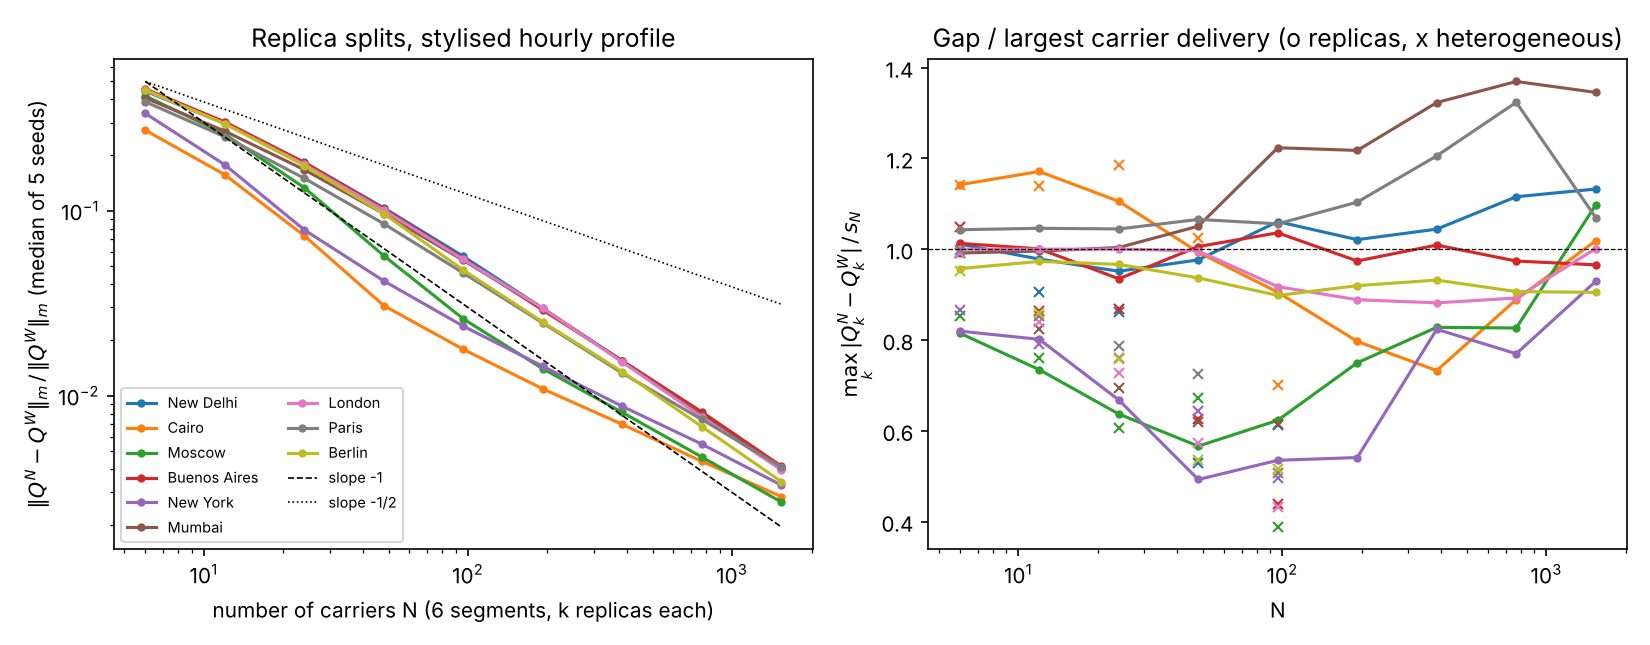
\includegraphics[width=\textwidth]{mfg_gap.png}
\caption{Left: relative aggregate gap against the number of carriers (replicas, median of five seeds). Right: largest coordinate gap in units of the largest carrier delivery $s_N$ (circles: replicas; crosses: heterogeneous splits).}\label{fig:gap}
\end{figure}

\begin{figure}[t]
\centering
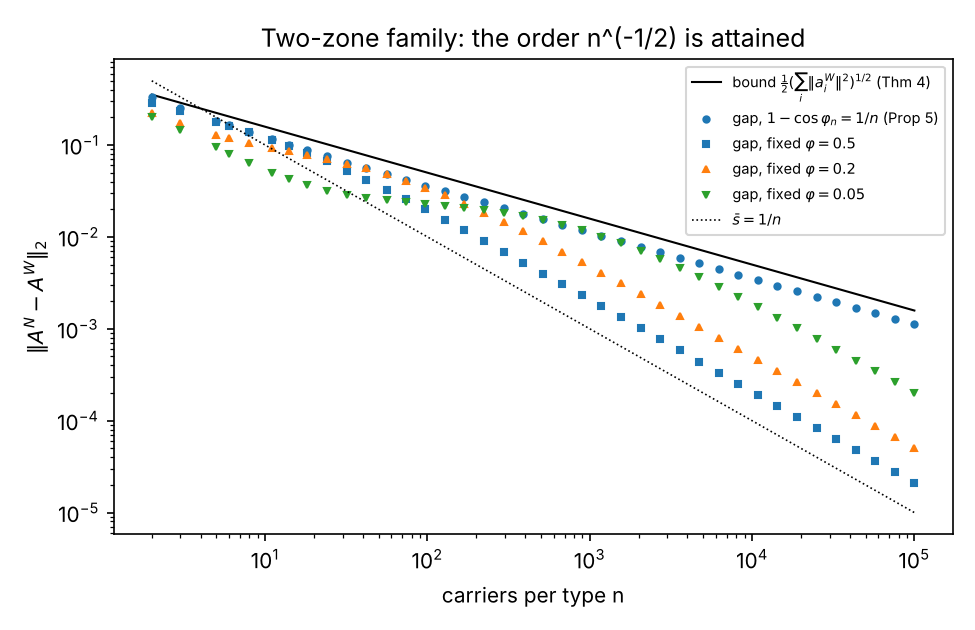
\includegraphics[width=0.62\textwidth]{mfg_tight.png}
\caption{The two-zone family of Proposition~\ref{prop:tight}. With $1-\cos\varphi_n=1/n$ the gap follows the bound of Theorem~\ref{thm:sqrt} at ratio $1/\sqrt2$; for a fixed angle it eventually falls like $1/n$, with a constant $1/\sin\varphi$.}\label{fig:tight}
\end{figure}

\paragraph{E2: the charge and the welfare} The calibrated congestion is weak relative to demand: $\varrho$ lies between \RhoMin{} and \RhoMax{}, the mean-field price of anarchy is \PoaWMed\% of optimal welfare (median; maximum \PoaWMax\%), and the welfare cost of the finite market is almost entirely Cournot withholding: PoA$-1$ is \PoaSixMed\% at $N=6$ (range \PoaSixMin--\PoaSixMax\%) and \PoaBigMed\% at $N=1536$ (Figure~\ref{fig:toll}). The observation-only fixed point approaches the Pigou charge with slope \SlopeToll{} $[\SlopeTollLo,\SlopeTollHi]$ (calibrated) and \SlopeTollK{} $[\SlopeTollKLo,\SlopeTollKHi]$ (congestion $\times10$, $\varrho$ up to \RhoKMax{}). The welfare bound of Theorem~\ref{thm:welfare}(b) held in \WelfOK{} instances; the realised loss was at most \WlossRatioMax{} of the bound.

The negative result is the leader gain. With few carriers the observation-only charge \emph{lowers} welfare: median $\GainSixMed\%$ at $N=6$ (calibrated) and $\GainKSixMed\%$ with congestion $\times10$, because it taxes deliveries that Cournot carriers already withhold. With congestion $\times10$ the gain is positive in every city and seed from $N=\GainKPosN$ on and reaches \GainKBigMed\% at $N=1536$ against \GainKWMed\% in the limit. With the calibrated congestion the attainable gain is tiny (\GainWMed\% in the limit) and the charge never helps in all instances at once. The Omega flat rule, which adds the market-power subsidy, is the right rule for few carriers (E5).

\begin{figure}[t]
\centering
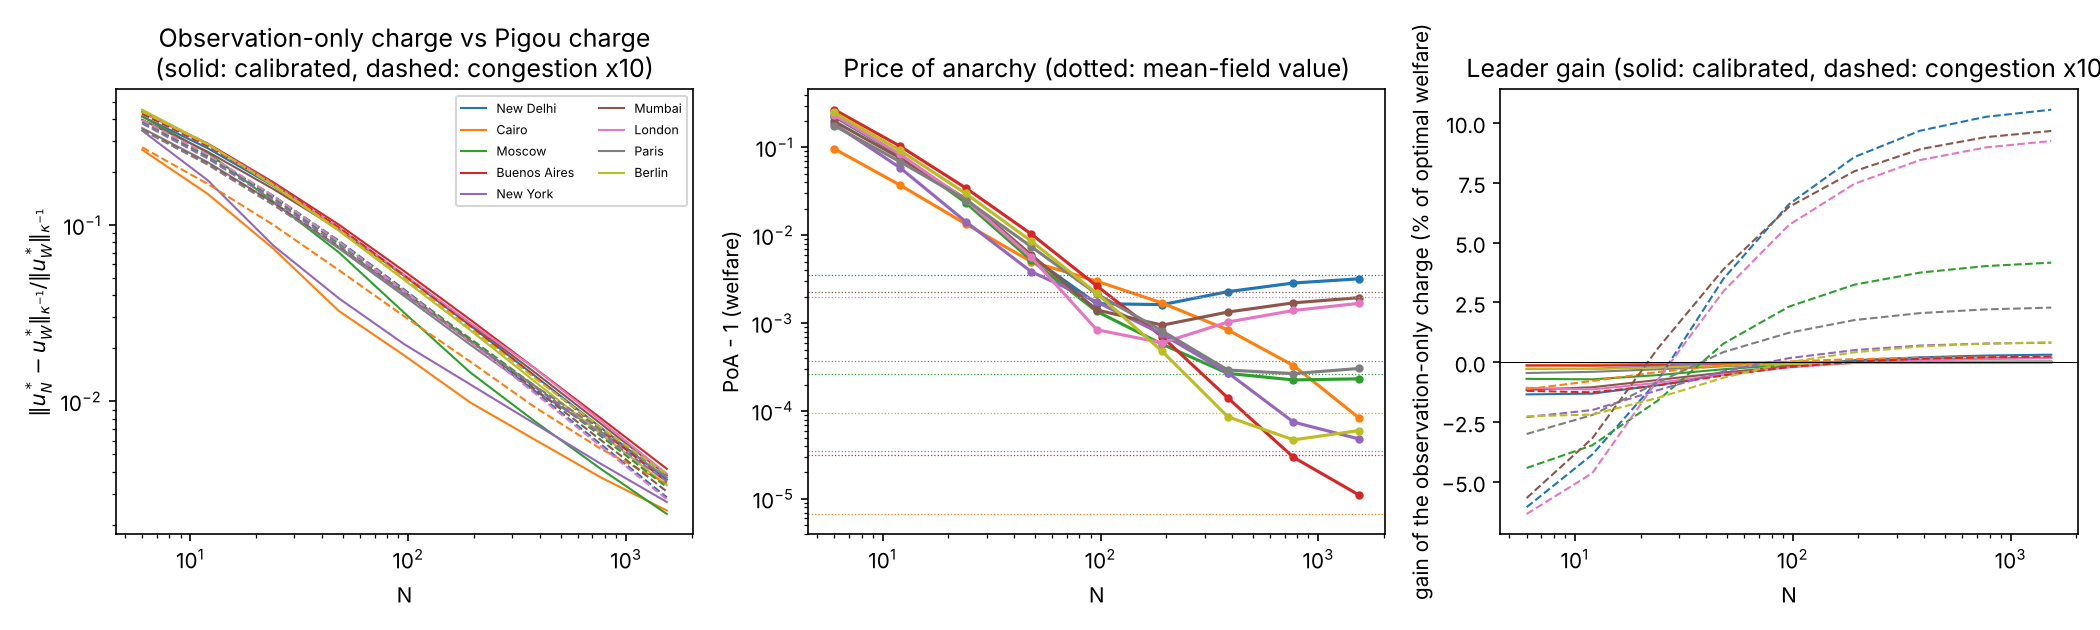
\includegraphics[width=\textwidth]{mfg_toll_poa.png}
\caption{Left: distance of the finite-market observation-only charge from the Pigou charge. Middle: price of anarchy at $N$ carriers (dotted: limit). Right: welfare gain of the observation-only charge (solid: calibrated congestion; dashed: congestion $\times10$).}\label{fig:toll}
\end{figure}

\paragraph{E3: the hourly profile matters little for these questions} With amplitudes $0$, $0.5$, $1$ and $1.5$ the median PoA$-1$ at $N=6$ is \PoaAmpZero, \PoaAmpHalf, \PoaAmpOne{} and \PoaAmpOneHalf\%, and the pooled gap slopes are \SlopeAmpZero, \SlopeAmpHalf, \SlopeAmpOne{} and \SlopeAmpOneHalf{} (Figure~\ref{fig:profile}). The convergence results do not depend on the profile, as the theory predicts (the bounds are uniform in the data), and the economic quantities move by about one percentage point. This is a weak result in the sense that it says little about real time-of-day effects: with a stylised profile, it shows only that our conclusions are not artefacts of a particular shape.

\begin{figure}[t]
\centering
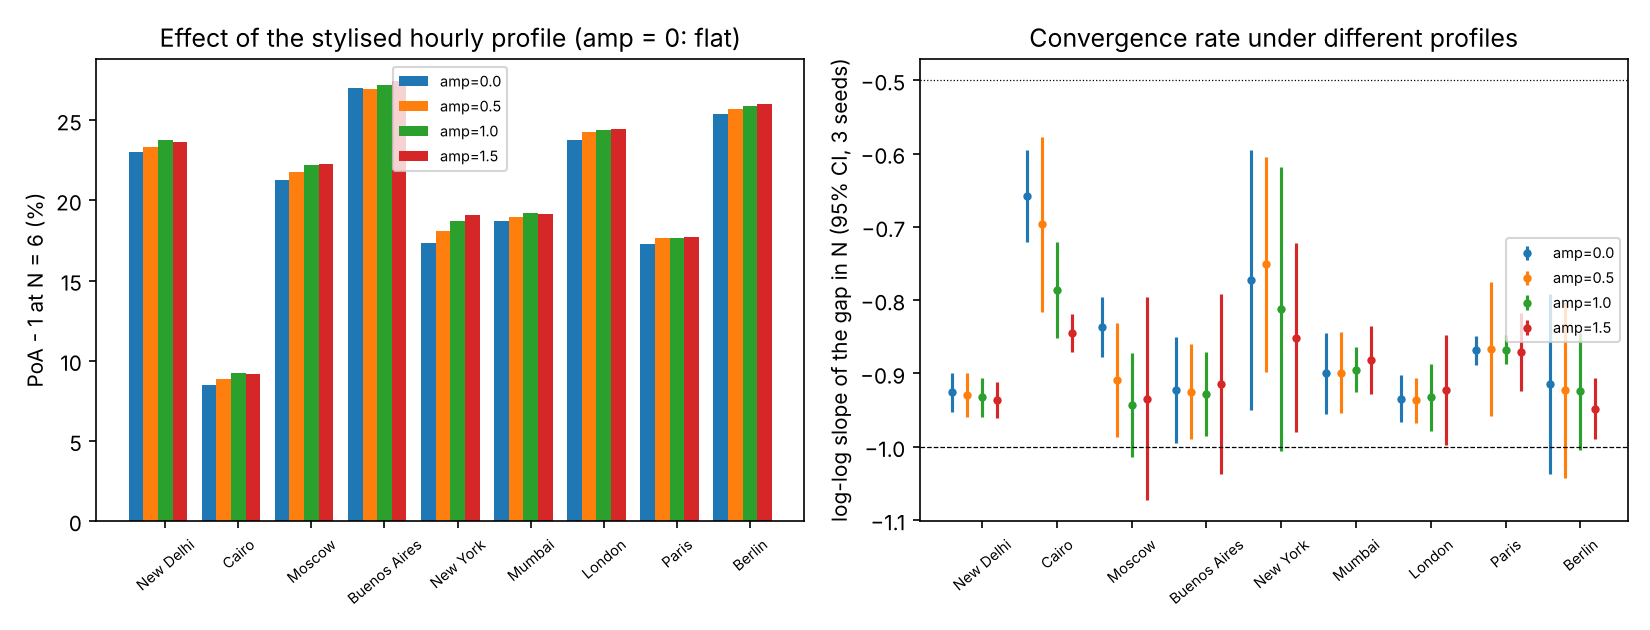
\includegraphics[width=\textwidth]{mfg_profile.png}
\caption{Sensitivity to the amplitude of the stylised hourly profile (three seeds). Left: PoA$-1$ at $N=6$. Right: gap slopes with 95\% intervals.}\label{fig:profile}
\end{figure}

\paragraph{E4: cautious carriers and the belief width} With the belief box in units of the median lot, the mean-field aggregate moves by at most \GamDevMax{} of the bound $\delta\norm w_m$ of Proposition~\ref{prop:gamma}(b) (median \GamDevMed). The observation-only charge under cautious carriers loses \GamLossOneMed\% of optimal welfare at $\delta=1$ and \GamLossFourMed\% at $\delta=4$ (median), within the bound of Proposition~\ref{prop:gamma}(d) in \GamLossOK{} cases (median ratio \GamLossRatioMed); the charge shift satisfied part (c) in \GamTollOK{} cases (Figure~\ref{fig:gamma}). The absorption width of Corollary~\ref{cor:width}, relative to the mean demand of a zone-hour, falls from \WidthSixMed{} at $N=6$ to \WidthBigMed{} at $N=24576$ (Figure~\ref{fig:width} in the appendix); with $d$ between \Dmin{} and \Dmax{} active zone-hours the $N$-free terms bind only beyond a few hundred carriers. This is a weak result: the uniform bound uses the largest delivery a carrier \emph{could} make at one zone-hour (its whole fleet there), and even with twenty-four thousand carriers it remains of the order of a zone-hour's demand, so the absorption theorem does not give a practically small belief width on these instances.

\begin{figure}[t]
\centering
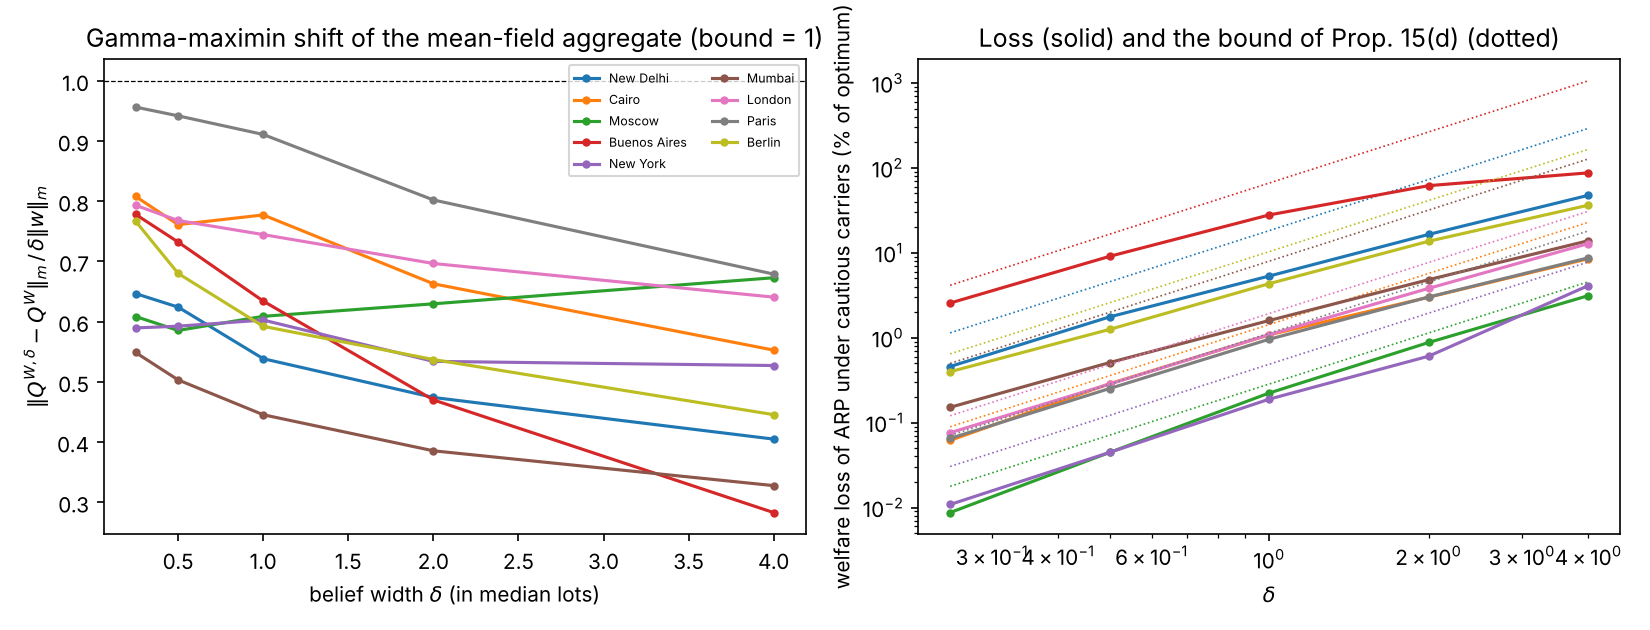
\includegraphics[width=\textwidth]{mfg_gamma.png}
\caption{$\Gamma$-maximin carriers ($N=1536$). Left: shift of the mean-field aggregate relative to the bound. Right: welfare loss of the observation-only charge and the bound $\tfrac12\delta^2\norm{m\odot w}^2_{(m+\kappa)^{-1}}$.}\label{fig:gamma}
\end{figure}

\paragraph{E5: which observation-only rule} Figure~\ref{fig:arp} (right) compares the observation-only Pigou rule with the Omega flat rule $u\leftarrow\kappa Q-m\odot\bar d$, where $\bar d$ is the observed mean delivery per active carrier (damped iteration). At $N=6$ the flat rule gains \FlatSixMed\% (calibrated; \FlatKSixMed\% with congestion $\times10$) where the Pigou rule loses \ObsSixMed\% (\ObsKSixMed\%); at $N=1536$ the flat rule gains \FlatBigMed\% (\FlatKBigMed\%) and its charge is within \FlatKDistBig{} (relative, congestion $\times10$) of the Pigou charge. The subsidy vanishes like the share, so the two rules meet in the limit. The plain rule contracted in every run at a per-round ratio of at most \PathRatioMax{} times $\varrho$, counting the rounds before the distance reached $10^{-6}$ of its initial value, below which solver accuracy dominates (left panel).

\begin{figure}[t]
\centering
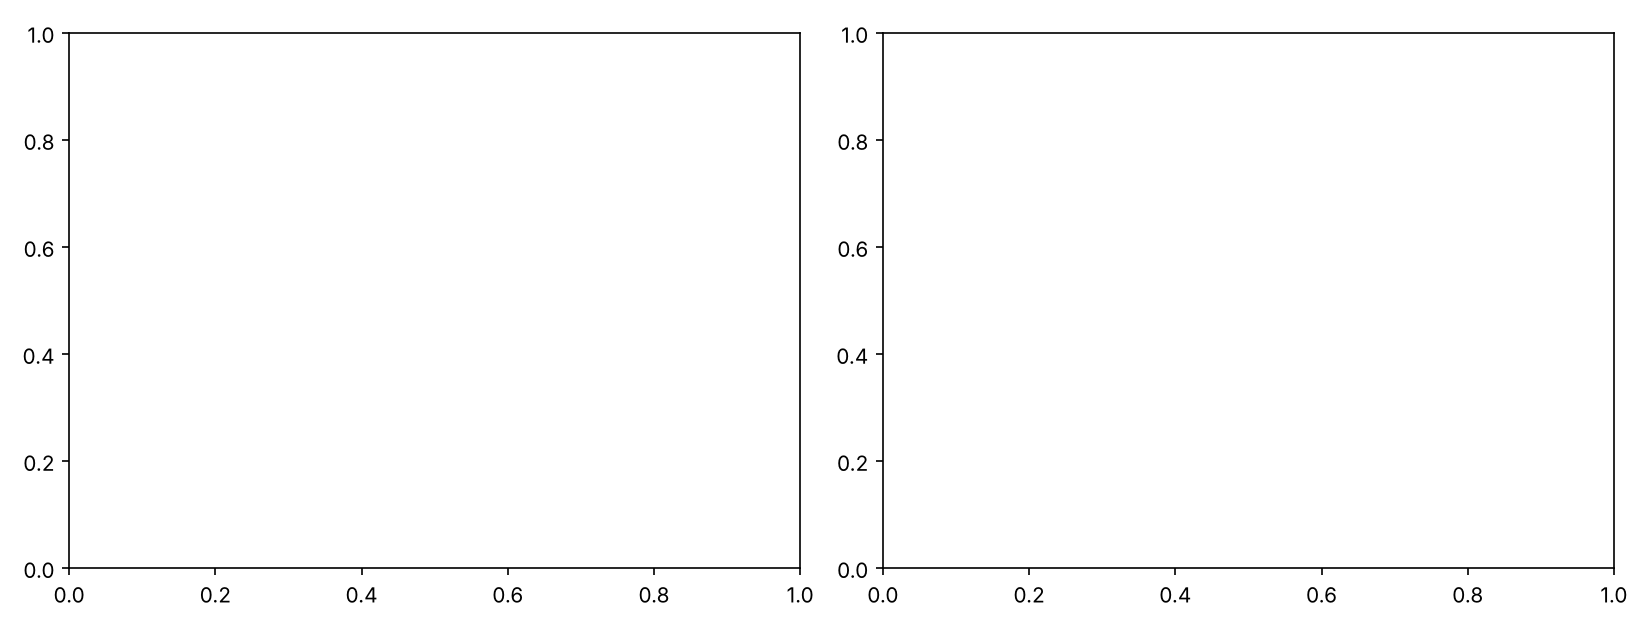
\includegraphics[width=\textwidth]{mfg_arp.png}
\caption{Left: plain observation-only iteration (Nash carriers), distance to the fixed point. Right: welfare gain of the Omega flat rule and of the observation-only Pigou rule against $N$ (median over cities and seeds).}\label{fig:arp}
\end{figure}

\paragraph{E6: cost} The replica reduction makes the Nash equilibrium for $N=1536$ as cheap as for $N=6$ (well under a second per program). Heterogeneous splits grow with $N$: at $N=96$ one interior-point solve took up to 90 seconds (Wardrop, whose solution set in the individual variables is not a singleton) and about 20 seconds (Nash). Plain Frank--Wolfe is slow: within 3000 rounds it reached a relative duality gap of $10^{-4}$ in \FWReached{} runs, and its relative gap after 3000 rounds was between \FWGapMin\% and \FWGapMax\% of the potential (Figure~\ref{fig:cost} in the appendix). It is adequate as a model of how a decentralised market adjusts, not as a solver for the precision that the rate study needs; all reported equilibria come from the interior-point method.

%======================================================================
% Section: who gains and who loses (input by mfg/paper/main.tex); numbers from mfg/paper/numbers_stake.tex
\section{Who gains and who loses}\label{sec:stake}

The welfare results above add up three groups: carriers, buyers of deliveries and the city. This section separates them. The accounting is that of Section~\ref{sec:model}: in zone-hour $k$ the price is $\alpha_k-b_kQ_k$, a delivery carries the delay cost $\kappa_kQ_k$, and the city posts a charge $u_k$ per delivery. For a profile with aggregate $Q$ and carrier profit vector $\pi$,
\begin{align*}
\text{consumer surplus } \mathrm{CS}&=\tfrac12\ip{b}{Q^2}, & \text{congestion cost } \mathrm{CC}&=\ip{\kappa}{Q^2},\\
\text{charge revenue } R&=\ip{u}{Q}, & \text{carrier profit } \Pi&=\sum_i\pi_i-\ip{b}{Q^2}-\mathrm{CC}-R,
\end{align*}
and $\SW=\mathrm{CS}+\Pi+R$ exactly (unit test in \texttt{mfg/tests/test_stake.py}; the identity holds to \StakeIdErr{} relative error in all \StakeRows{} instances). Charges are a transfer: they move welfare between $\Pi$ and $R$ and change $\SW$ only through the deliveries. In this model the delay cost is borne by the delivery fleet, so residents carry no monetary congestion cost; their stake is the demand side (CS) and, in Section~\ref{sec:residents}, the vehicle-hours spent in their zone.

\paragraph{Three rules} All rules are evaluated at the Nash equilibrium of the finite market under the posted charge, on the instances of Section~\ref{sec:exp} (nine cities, five seeds, $N=6k$, $k=1,\dots,256$). \emph{No charge}: $u=0$. \emph{Observation-only}: the finite-market fixed point $u=\kappa\odot Q(u)$ of Proposition~\ref{prop:arp}, the Pigou charge without any market-power correction. \emph{Pigou minus market power} (the rule of the Omega paper): $u=\kappa\odot Q^\opt-m\odot\bar a$, with $\bar a_k$ the optimum's delivery per active carrier, corrected for 25 damped rounds $u\leftarrow u+0.8\,m\odot(1+1/n_k)\odot(Q(u)-Q^\opt)$ ($n_k$ the number of active carriers) so that the Nash aggregate matches $Q^\opt$; the median relative $M$-norm residual of the match is \PmResidMed{} (maximum \PmResidMax). This rule solves for a charge that reproduces the optimal aggregate; with several carrier types it need not reproduce the optimal individual plans, so it can fall short of $\SW^\opt$ (median welfare shortfall \PmLossSix\% at $N=6$ and \PmLossBig\% at $N=1536$).

\subsection{The charge that implements the optimum}\label{sec:ident}
For one segment split into $N$ identical carriers the optimal charge has a closed form.

\begin{proposition}[Pigou minus market power]\label{prop:marketpower}
Let the $N$ carriers be identical replicas of one type (Lemma~\ref{lem:rep}) and let $Q^\opt$ be the aggregate of a social optimum. The charge
\[
u^*_N=\kappa\odot Q^\opt-\tfrac1N\,m\odot Q^\opt
\]
makes the Nash equilibrium aggregate equal to $Q^\opt$ and its welfare equal to $\SW^\opt$, for any coupling of the plans across zone-hours. It is the Pigou charge $\kappa\odot Q^\opt$ minus a market-power term of exact size $\tfrac1N m_kQ^\opt_k$. Coordinate $k$ is taxed if $N>m_k/\kappa_k=1/\varrho_k$ and subsidised if $N<1/\varrho_k$. In the one-zone case with unconstrained deliveries, $Q^\Nash=\frac N{N+1}Q^\War$, $Q^\War=\alpha/m$, $Q^\opt=\alpha/(m+\kappa)$ and $u_N^*=\alpha(\kappa-m/N)/(m+\kappa)$.
\end{proposition}
\begin{proof}
By Lemma~\ref{lem:rep} with one type, the type total $Y$ of a Nash equilibrium maximises $\Phi(Y)=\pi(Y)-\ip{u}{A}-\tfrac12(1+\tfrac1N)\norm{A}_m^2$, $A=LY$, over the (convex) fleet polytope, and each carrier delivers $A/N$. At $u=u_N^*$ the gradient of $\Phi$ at the social optimum $Y^\opt$ is $\nabla\pi-L^\top[(\kappa-\tfrac mN)\odot Q^\opt+(1+\tfrac1N)m\odot Q^\opt]=\nabla\pi-L^\top[(m+\kappa)\odot Q^\opt]$, which is the gradient of the social objective $\pi-\tfrac12\norm{A}_{m+\kappa}^2$ at $Y^\opt$. The variational inequality of $Y^\opt$ for the social problem is therefore that of $\Phi$; $\Phi$ is concave, so $Y^\opt$ maximises it, and the Nash aggregate is unique (Lemma~\ref{lem:pot}(b)). Welfare depends on the profile only through $\pi$ and $Q$. The one-zone formulas: the Nash first-order condition $\alpha-u=(1+\tfrac1N)mQ$ gives $Q^\Nash=\frac N{N+1}\alpha/m$ at $u=0$, and $u=\alpha-(1+\tfrac1N)m\frac{\alpha}{m+\kappa}=\alpha\frac{\kappa-m/N}{m+\kappa}$ at $Q=Q^\opt$.
\end{proof}

The proposition was checked on the nine cities with one segment per city (three seeds, $N=1,2,3,6,\dots,1536$, \IdRows{} instances): the Nash aggregate under $u_N^*$ equals $Q^\opt$ to a relative $M$-norm error of at most \IdQErr{} and the welfare to \IdSWErr{}, while without a charge a single-segment market loses \IdSixNone\% of optimal welfare at $N=6$ (median) and the pure Pigou charge \IdSixPig\%; at $N=1536$ the losses are \IdBigNone\% and $4\cdot10^{-5}\%$. The charge is a subsidy in every zone-hour at $N=6$ and in \IdOneNinetyTwoSub\% of them at $N=192$; its size relative to the Pigou charge is \IdSixRatio{} at $N=6$ (the sum over zone-hours, a net subsidy) and \IdBigRatio{} at $N=1536$. The one-zone relation $Q^\Nash=\frac N{N+1}Q^\War$ is exact only while the fleet budget is slack: it holds to $10^{-9}$ in six of the nine cities and deviates by up to \IdRatioDevMax\% elsewhere, where the budget binds; the charge formula does not depend on it. For several carrier types the charge $u^*_N$ is not available, because the market-power terms $m\odot a_\theta$ differ across types and one posted charge cannot cancel all of them; the rule above is the numerical substitute.

\subsection{The city council}\label{sec:council}
Table~\ref{tab:stake_who} gives, for the four sizes $N\in\{6,24,192,1536\}$ and the two rules that charge, the change of each term relative to no charge, as a percentage of welfare without charge (medians over nine cities and five seeds; city values in \texttt{results/summary\_stake\_who\_city.csv}). Figure~\ref{fig:stake_who} shows all nine sizes.

\begin{table}[t]
\centering\footnotesize\setlength{\tabcolsep}{4pt}
\caption{Change with respect to no charge, in \% of welfare without charge (median of 45 instances). $\Delta\Pi$: carrier profit net of the charge; $\Delta$CS: consumer surplus; $\Delta$CC: congestion cost; $R$: charge revenue (negative: subsidy paid by the city); $\Delta\SW=\Delta\Pi+\Delta\mathrm{CS}+R$ up to medians; last column: $R$ as a share of the welfare under the rule.}\label{tab:stake_who}
\begin{tabular}{rlrrrrrr}
\toprule
$N$ & rule & $\Delta\Pi$ & $\Delta$CS & $\Delta$CC & $R$ & $\Delta\SW$ & $R/\SW$\\
\midrule
6 & observation-only & -1.1 & -1.0 & 0.0 & +1.6 & -0.5 & +1.6 \\
 & Pigou minus market power & +132.0 & +69.1 & +2.2 & -181.9 & +19.6 & -151.9 \\
\addlinespace
24 & observation-only & -0.7 & -2.4 & -0.1 & +2.7 & -0.3 & +2.8 \\
 & Pigou minus market power & +13.4 & +21.6 & +0.7 & -36.9 & +1.9 & -36.1 \\
\addlinespace
192 & observation-only & -0.4 & -1.8 & -0.1 & +3.3 & 0.0 & +3.3 \\
 & Pigou minus market power & +0.3 & +0.1 & 0.0 & -1.9 & 0.0 & -1.9 \\
\addlinespace
1536 & observation-only & -0.1 & -1.6 & -0.1 & +3.4 & 0.0 & +3.4 \\
 & Pigou minus market power & -0.1 & -1.1 & -0.1 & +3.0 & 0.0 & +3.0

\bottomrule
\end{tabular}
\end{table}

\begin{figure}[t]
\centering
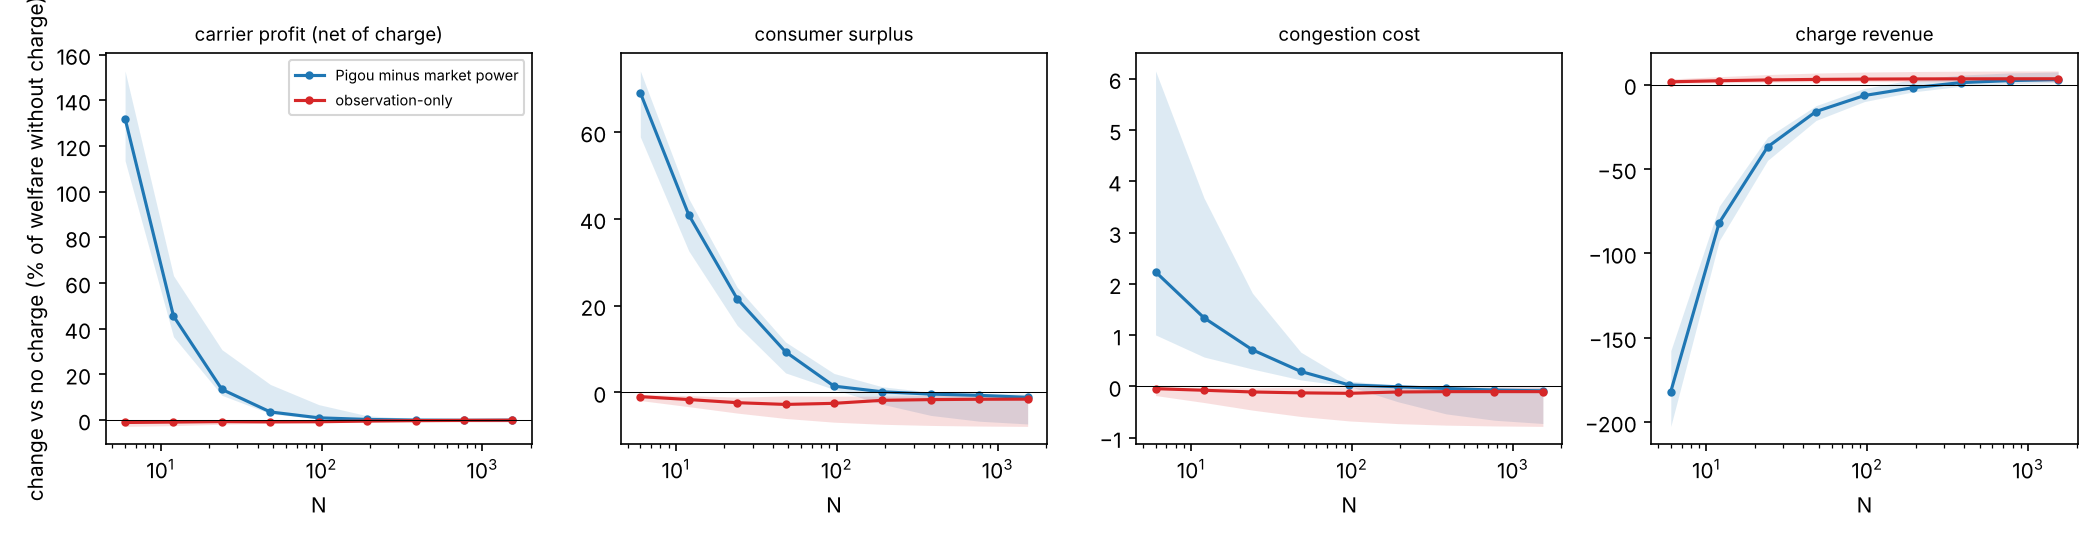
\includegraphics[width=\textwidth]{mfg_stake_who.png}
\caption{Change of each welfare term against no charge (\% of welfare without charge; median and interquartile range over nine cities and five seeds). Blue: Pigou minus market power; red: observation-only.}\label{fig:stake_who}
\end{figure}

\paragraph{Revenue} With many carriers the council collects about \WBigObsR\% of welfare under either rule (the Pigou charge in the limit), \WBigPmRshare\% under the market-power rule at $N=1536$. With few carriers the picture reverses. The observation-only charge still raises \WSixObsR\% of welfare but lowers welfare by \WSixObsdSW\% (it taxes deliveries that Cournot carriers already withhold), whereas the market-power rule raises welfare by \WSixPmdSW\% at a net \emph{cost} to the council: its revenue is $\WSixPmR\%$ of the no-charge welfare, i.e.\ \WSixPmRshare\% of the welfare under the rule, and it is negative in \PmSubsidyInst{} instances. The efficient charge at $N=6$ is a subsidy to carriers in about \PmNegShare\% of zone-hours; it removes the market power by paying carriers to deliver more. At $N=24$ the subsidy is still $36.9\%$ of the no-charge welfare and it falls under $2\%$ at $N=192$. A council that cannot run a deficit has to recover the transfer by a lump-sum fee (a fixed licence fee does not change the deliveries; not modelled here), or settle for a smaller correction. Budget neutrality is thus a property of large markets only.

\paragraph{One city-wide charge or zone-hour charges?} The market-power charge is posted per zone and hour. If the council may post a single per-delivery charge $\bar u$ for the whole city, the best scalar (found by a grid and a bounded search; \texttt{results/uniform.csv}) leaves a welfare loss of \UnSixUni\% of the optimum at $N=6$ against \UnSixPm\% for zone-hour charges and \UnSixNone\% without charge; it captures \UnSixFrac\% of the gain of the zone-hour rule (median; range \UnSixFracMin--\UnSixFracMax\%). The best scalar is negative, a subsidy, for small $N$ and turns positive near $N=16$ to $32$. In the mean-field limit the loss of the best single charge is \UnWUni\% of the optimum (maximum \UnWUniMax\%) against $0$ for zone-hour charges, and no charge loses \UnWNone\%: the best city-wide charge captures \UnWFrac\% of the possible gain (range \UnWFracMin--\UnWFracMax\%). Differentiated charges therefore matter most where the calibrated congestion slopes differ most across zone-hours; with this calibration the welfare at stake in the choice is small in absolute terms.

\paragraph{A wrong charge} Let the council post $(1+\varepsilon)$ times the Pigou charge, $\varepsilon\in\{\pm10\%,\pm25\%\}$, in the mean-field market. Theorem~\ref{thm:welfare}(a) bounds the loss by $\tfrac12\norm{v-\kappa\odot Q^\opt}_{b^{-1}}^2=\tfrac12\varepsilon^2\norm{\kappa\odot Q^\opt}^2_{b^{-1}}$. Measured, the median loss is \MisTenLoss\% of the optimum for $|\varepsilon|=10\%$ and \MisTwentyFiveLoss\% for $25\%$; the bound held in \MisHeld{} instances and the measured loss was between \MisTwentyFiveRatioMin{} and \MisTwentyFiveRatioMax{} of the bound (median \MisTwentyFiveRatio) at $25\%$ (\MisTenRatioMin--\MisTenRatioMax{} at $10\%$). The first inequality of the theorem, which uses the realised aggregate, is almost an equality (the loss equals it to $10^{-5}$ of welfare in \MisHeldTight{} cases). Losses grow with $\varepsilon^2$, as the bound says: a $10\%$ error costs a sixth of what a $25\%$ error costs. With few carriers the same errors matter more because the market-power correction is itself a subsidy of the order of the welfare: with the market-power charge scaled by $1\pm25\%$ the Nash welfare loss rises from \PmLossSix\% to \MisNSixTwentyFive\% at $N=6$ and is \MisNBigTwentyFive\% at $N=1536$.

\subsection{Residents}\label{sec:residents}
Residents appear twice: as buyers (consumer surplus) and as people who live next to the delivery vehicles. As buyers, they are the main beneficiaries of the market-power correction: at $N=6$ consumer surplus rises by \WSixPmdCS\% of welfare under the market-power rule (city medians from \WSixPmCSMin\% to \WSixPmCSMax\%), because deliveries are priced lower and more are made, and it falls by \WSixObsdCS\% under the observation-only charge, which raises the price. At $N=1536$ both rules take about \WBigPmdCS\% of welfare from consumers (city range \WBigObsCSMin\% to \WBigObsCSMax\% under the observation-only rule), the price of the congestion that the charge removes; the decline of congestion cost, \WBigPmdCC\%, is smaller than the loss in consumer surplus and the council's revenue is the rest.

\paragraph{The burden of congestion is small in this calibration} Without charge the congestion cost is \LSixCCshare\% of welfare at $N=6$ and \LBigCCshare\% at $N=1536$ (largest city \LBigCCshareMax\%), against consumer surplus of \LSixCSshare\% and \LBigCSshare\% of welfare. The vehicle-hours that deliveries add in residents' zones are also small: with the stylised dwell time of $r$ hours per delivery, the delivery vehicles spend on average \ExpBigMean{} vehicle-minutes per resident and day in the zones they serve at $N=1536$ (\ExpSixMean{} at $N=6$, where withholding cuts volume).

\begin{table}[t]
\centering\footnotesize\setlength{\tabcolsep}{4pt}
\caption{Exposure of residents of the served zones (median of 45 instances). Exposure: delivery vehicle-hours in the resident's zone per resident, scaled to the real city (in-zone dwell only). Mean: vehicle-minutes per resident and day, population-weighted; Gini: population-weighted Gini of daily exposure by zone, and of exposure by zone-hour; D10/D1: mean exposure of the most exposed tenth of residents over that of the least exposed tenth; $\rho_s$: Spearman correlation across zones, within an instance, of the relative change of a zone's share of vehicle-hours against the log of its population density (change from no charge).}\label{tab:stake_exposure}
\begin{tabular}{rlrrrrr}
\toprule
$N$ & rule & mean & Gini zone & Gini zone-hour & D10/D1 & $\rho_s$\\
\midrule
6 & no charge & 0.160 & 0.135 & 0.314 & 2.25 & -- \\
 & observation-only & 0.159 & 0.134 & 0.313 & 2.22 & -0.56 \\
 & Pigou minus market power & 0.278 & 0.080 & 0.289 & 1.90 & -0.03 \\
\addlinespace
1536 & no charge & 0.281 & 0.080 & 0.291 & 1.91 & -- \\
 & observation-only & 0.277 & 0.080 & 0.288 & 1.91 & -0.59 \\
 & Pigou minus market power & 0.278 & 0.080 & 0.288 & 1.91 & -0.56

\bottomrule
\end{tabular}
\end{table}

\paragraph{Inequality of exposure} Table~\ref{tab:stake_exposure} gives the exposure measures with the GHSL population of each zone (population only: the repository has no income data, so nothing here speaks to income equity). Exposure is already fairly even across the served zones: Gini \ExpBigGiniNone{} at $N=1536$ and a ratio of top to bottom decile of \ExpBigDtenNone. At $N=1536$ the charges leave the Gini of daily exposure unchanged to the third decimal (change \ExpBigObsdGini{} under the observation-only rule, \ExpBigPmdGini{} under the market-power rule; tenth to ninetieth percentile of instances \ExpBigObsdGiniMin{} to \ExpBigObsdGiniMax{}). At $N=6$ the market-power rule lowers the Gini by \ExpSixPmdGini{} and the decile ratio by \ExpSixPmdDten, but this comes from the larger volume (withholding is worst where the zone's demand is thin) and not from the congestion charge; the observation-only rule changes it by \ExpSixObsdGini.

\paragraph{Does the charge push traffic towards dense zones?} No, in this model it does the opposite. The charge is proportional to the zone-hour's congestion slope, and the zones with high density and demand have the steeper slopes. Across zones the relative change of a zone's share of vehicle-hours is negatively rank-correlated with the zone's population density (median Spearman $\rho_s=\ExpBigPmCorr$ at $N=1536$, \ExpBigPmCorrNeg{} instances negative, tenth to ninetieth percentile \ExpBigPmCorrMin{} to \ExpBigPmCorrMax; observation-only $\ExpBigObsCorr$). Dense zones lose share, sparse zones gain it; the shift in the mean log density of exposure is \ExpBigPmShift. The exception is $N=6$ under the market-power rule, where every zone's volume rises and the correlation vanishes ($\ExpSixPmCorr$). The effect is small in size, since the zone-hour charges move total vehicle-hours by only \ExpBigPmdExp\% at $N=1536$. The covered zones are the 8 customer zones of each of six segments; the statistics describe those zones, not the whole city.

\subsection{Businesses}\label{sec:businesses}
Businesses here are the delivery carriers; shippers and shops are not modelled, so their interest enters only through the demand curve. The first-best correction is good for them at small $N$ only because of the subsidy: at $N=6$ carrier profit net of the charge rises by \WSixPmdPi\% of the no-charge welfare under the market-power rule, where the subsidy is $|R|=\WSixPmR\%$; gross of the transfer, operating profit falls and the fleet's delay cost rises slightly (\WSixPmdCC\%), as more deliveries are made at a lower price. Under the observation-only rule carriers lose \WSixObsdPi\% at $N=6$ and \WBigObsdPi\% at $N=1536$, almost nothing, because their payments are close to the cost they impose on each other. The ranking of the council's options from the carriers' side is therefore the reverse of the one from consumers' side only for the observation-only rule; for the market-power rule the carriers and the consumers both gain at small $N$ and the council pays. In large markets the two rules coincide, carriers lose \WBigPmdPi\% (city medians from \WBigObsPiMin\% to \WBigObsPiMax\% of welfare for the observation-only rule), and the charge falls on consumers, as in any pass-through of a per-delivery charge to a market with a downward-sloping demand.

\paragraph{Limitations of the stakeholder reading} Consumer surplus is model-based: it is the integral under the linear inverse demand $\alpha_k-b_kQ_k$ calibrated on the delivery fee, not a measured willingness to pay. There are no income data, so the exposure statistics are about population, not about who is poor. The number of carriers is fixed: the charge does not induce entry or exit, and a subsidy of the size needed at $N=6$ would in practice attract entrants, which the model cannot show. The calibrated congestion is weak (congestion cost is \LBigCCshare\% of welfare at $N=1536$) so that the congestion side of every table is small; the entries scale with the congestion slope, and with congestion ten times higher (Section~\ref{sec:exp}) the observation-only charge gains from $N=192$ and the residents' side would be larger, but this was not rerun for the tables above. Exposure counts in-zone delivery hours only and leaves out through traffic, noise and emissions. The covered zones are those that the six drawn segments serve.

% Section: fixed fees, entry and other externalities (input by mfg/paper/main.tex); numbers from numbers_ext.tex
\section{Fixed fees, entry and other externalities}\label{sec:ext}
Section~\ref{sec:stake} left three questions open: who pays for the subsidy that the efficient charge contains when carriers are few, what the subsidy and the charge do to the number of carriers, and what changes when delivery traffic causes costs other than in-zone delay.

\subsection{Recovering the subsidy with a fixed fee}\label{sec:fees}
Let the city post a charge $u$ per delivery and, in addition, collect a fee $T_i$ from carrier $i$. Call the fee \emph{lump-sum} if it is fixed before carriers choose their plans: it may depend on the carrier's identity, its licensed fleet or the plan the city is aiming at, but not on the deliveries the carrier actually makes.

\begin{proposition}[Lump-sum fees]\label{prop:fee}
Fix the set of $N$ carriers, a charge $u$ and outside options $\underline\pi_i$.
\begin{enumerate}
\item[(a)] With lump-sum fees the Nash equilibria are those without fees. Deliveries, consumer surplus, congestion cost and welfare are unchanged; the fees move $\sum_iT_i$ from carriers to the city.
\item[(b)] All carriers stay in the market iff $\pi_i(u)-T_i\ge\underline\pi_i$ for every $i$, where $\pi_i(u)$ is carrier $i$'s equilibrium profit net of the charge. Fees with $\sum_iT_i=D$ and participation exist iff $\sum_i(\pi_i(u)-\underline\pi_i)\ge D$; for the deficit $D=-R$ of the charge and $\underline\pi_i=0$ this reads $\Pi_{\rm op}-\mathrm{CC}\ge0$, operating profit net of the delay cost at the target.
\item[(c)] A fee that recovers the \emph{realised} deficit, $T_i=-\ip{u}{Q}/N$, is not lump-sum. Carrier $i$ then faces the charge $(1-\tfrac1N)u$ on its own deliveries, and in the one-zone case of Proposition~\ref{prop:marketpower} the Nash aggregate under $u=u_N^*<0$ falls below $Q^\opt$.
\end{enumerate}
\end{proposition}
\emph{The proof is in Appendix~\ref{app:proofs}.}

The proposition is elementary; for the city, (b) and (c) say that the fee must be computed from the target plan, not from the books after the fact, and must leave each carrier its outside option. Table~\ref{tab:fees} applies it to the market-power rule of Section~\ref{sec:stake} with outside option zero. At $N=6$ the deficit is \FeeSixDef\,\% of welfare (median) and the charge is a subsidy in \FeeSixSub\,\% of zone-hours; recovering it takes \FeeSixShare\,\% of carrier profit (range \FeeSixShareMin--\FeeSixShareMax\,\%). A flat fee per carrier leaves some carrier with a loss in every instance (participation in \FeeSixFlatOK), a fee in proportion to the licensed fleet in \FeeSixFleetOK{} instances; carrier-specific fees exist in \FeeSixAggregateOK{} instances, the exceptions being \FeeAggFailCities, where the subsidy exceeds total carrier profit. At $N=24$ the fee takes \FeeTwentyFourShare\,\% of profit and a flat fee keeps every carrier in \FeeTwentyFourFlatOK{} instances; at $N=192$ the charge is a subsidy only in some cities and the fee takes \FeeOneNinetyTwoShare\,\% (participation \FeeOneNinetyTwoFlatOK{} flat); at $N=1536$ the charge raises revenue and no fee is needed. After the fee, carriers keep \FeeSixKept\,\% of their no-charge profit at $N=6$ (\FeeTwentyFourKept\,\% at $N=24$): the subsidy and the fee together transfer the Cournot rent to buyers, and for $N\le192$ no fee scheme leaves every carrier with at least its no-charge profit in any instance. Recovering the realised deficit instead (part (c)) costs \FeeSixEpLoss\,\% of optimal welfare at $N=6$, small because the residual subsidy is still $(1-\tfrac16)u$.



So the subsidy is budget-balanceable with participation only with carrier-specific fees at $N=6$, and with simple fees from about $N=192$ on, where it is small. With a fixed set of carriers this is about distribution; it stops being so when carriers can leave or enter.

\subsection{Entry and exit}\label{sec:entry}
\paragraph{Model} Segment $\theta$ has $k_\theta$ identical carriers that share its fleet budget $B_\theta$ (Section~\ref{sec:data}); the fleet is a pool of drivers and vans calibrated from demand, so entry adds firms, not vehicles. Each carrier pays a fixed cost $F_\theta$ per day (depot, licence, management; vehicle costs are in the tour cost). Counts are real numbers, a continuous approximation of the integer count; a segment whose single carrier cannot cover $F_\theta$ leaves the market. A \emph{free-entry equilibrium} under a charge rule is a Nash equilibrium with $\pi_\theta/k_\theta-T_\theta=F_\theta$ for every active segment, $\pi_\theta$ the segment's profit net of the charge and $T_\theta$ its fee per carrier. Welfare is $\SW-\sum_\theta k_\theta F_\theta$.

\begin{proposition}[Free entry]\label{prop:entry}
\begin{enumerate}
\item[(a)] At every free-entry equilibrium, under any charge and lump-sum fees, welfare net of fixed costs equals $\mathrm{CS}+R+\sum_\theta k_\theta T_\theta$: consumer surplus plus the city's net revenue. Of two rules that produce the same aggregate, the one with the larger net revenue has the larger welfare.
\item[(b)] One zone, $N$ identical carriers, slack budget, charge $u$, no fee. Every carrier delivers $s=(F/m)^{1/2}$ whatever $u$, and the free-entry number is $N^*(u)=(\alpha-u)/(mF)^{1/2}-1$. Under no charge $N_a=\alpha/(mF)^{1/2}-1$; under the observation-only rule $N_b=Q_b/s$ with $Q_b=(\alpha-ms)/(m+\kappa)$; under Pigou minus market power ($u=u^*_N$ of Proposition~\ref{prop:marketpower} with $N$ endogenous) $N_c=Q^\opt/s$; with the fee $T=-u Q^\opt/N$ recovering a subsidy, $N_d=\kappa(Q^\opt)^2/F$, smaller than $N_c$ exactly when the charge is a subsidy ($N_c<m/\kappa$).
\item[(c)] (Excess entry.) In (b) with $u=0$, welfare decreases in $N$ at $N_a$: a planner who could limit entry, but not change Cournot conduct, would admit fewer carriers.
\item[(d)] (Second best, one-zone linear case.) In (b), welfare net of fixed costs as a function of a constant charge $u$ is maximised at $u=\kappa Q_b$, the observation-only fixed point; the market-power term of $u^*_N$ is absent, and $u^*_N$ with endogenous $N$ gives lower welfare.
\end{enumerate}
\end{proposition}
\emph{The proof is in Appendix~\ref{app:proofs}.}

Part (c) is the business-stealing result of \citet{MankiwWhinston1986}; parts (a), (b) and (d) are short computations in the same model. The literature on taxes under free-entry oligopoly finds that the optimal specific tax departs from the Pigou level by a term of either sign that depends on the curvature of demand and costs \citep{Konishi1990,KatsoulacosXepapadeas1995,Hamada2022}. Part (d) holds in the one-zone linear case only: output per carrier is pinned down by $F$ alone, a charge changes only the number of carriers, and the departure is zero. The congestion-pricing literature with market power \citep{Brueckner2002,PelsVerhoef2004} gives the fixed-$N$ counterpart, a toll below the congestion cost and possibly negative, which is Proposition~\ref{prop:marketpower}, a finite-$N$ analogue of those results. With $N$ endogenous the market-power subsidy no longer buys output per carrier; it buys entrants.

\paragraph{Calibration of $F$} $F_\theta$ is not observed; we set it so that the no-charge free-entry count lies between $k_0$ and $k_0+1$ carriers per segment (the geometric mean of the profit per carrier at $k_0$ and $k_0+1$), for $N_0=6k_0\in\{6,24,192\}$ (three seeds, \EntInst{} city-seed pairs), and sweep $N_0\in\{12,48,96,384\}$ on seed 0. A smaller $N_0$ means a larger fixed cost. Zero-profit residuals are below $10^{-5}$ of $F$ except for the market-power rules, where \EntConv{} runs reached $10^{-4}$ and the rest stopped after 80 rounds (residual up to \EntErrMax{} of $F$, identity of Proposition~\ref{prop:entry}(a) to \EntIdErr{} of welfare); no reported sign depends on them.



\paragraph{Results} Table~\ref{tab:entry} and Figure~\ref{fig:entry}. \emph{The subsidy attracts entrants.} Under Pigou minus market power the count rises to \EntSixPmN{} at $N_0=6$ and \EntTwentyFourPmN{} at $N_0=24$, and welfare net of fixed costs changes by \EntSixPmdSW\,\% and \EntTwentyFourPmdSW\,\% against no charge (ranges \EntSixPmdSWMin{} to \EntSixPmdSWMax\,\% and \EntTwentyFourPmdSWMin{} to \EntTwentyFourPmdSWMax\,\%): the rule that gained \WSixPmdSW\,\% with six fixed carriers loses in every instance once entry responds, because the subsidy pays for fixed costs instead of output. \emph{The recovery fee drives exits.} With the fee the count falls to \EntSixPmfeeN{} at $N_0=6$ (median \EntSixPmfeeAct{} of six segments stay; the market closes in \EntSixPmfeeClosed{} instances) and to \EntTwentyFourPmfeeN{} at $N_0=24$ (\EntTwentyFourPmfeeAct{} segments). The fee raises the cost of being a carrier by about the subsidy each one receives (Proposition~\ref{prop:entry}(b)). Because free entry is excessive (below), the exits can raise welfare: the fee rule beats no charge in \EntSixPmfeeBeatsNone{} instances at $N_0=6$ and \EntTwentyFourPmfeeBeatsNone{} at $N_0=24$ (median \EntSixPmfeedSW{} and \EntTwentyFourPmfeedSW\,\%, ranges \EntSixPmfeedSWMin{} to \EntSixPmfeedSWMax\,\% and \EntTwentyFourPmfeedSWMin{} to \EntTwentyFourPmfeedSWMax\,\%); it acts as an uncontrolled entry restriction whose outcome ranges from closing the market to a large gain. \emph{The observation-only charge is safe and close to the second best.} It changes the count little (\EntSixObsN, \EntTwentyFourObsN, \EntOneNinetyTwoObsN), raises welfare and beats the market-power rule in every instance, and is the best of the scalings $\theta\in\{0.5,1,1.5\}$ in \EntSixObsBest, \EntTwentyFourObsBest{} and \EntOneNinetyTwoObsBest{} instances: the one-zone result of Proposition~\ref{prop:entry}(d) holds approximately, less so with many carriers. The gains are small (\EntSixObsdSW, \EntTwentyFourObsdSW{} and \EntOneNinetyTwoObsdSW\,\%) because the calibrated congestion is weak. The $F$ sweep in Figure~\ref{fig:entry} shows the same ordering at every $N_0$; the fee rule's median changes sign between $N_0=12$ and $N_0=24$.

\emph{Excess entry.} Scaling the no-charge free-entry counts by $\lambda$ (at least one carrier per segment, conduct unchanged), welfare net of fixed costs is largest at one carrier per segment for $N_0=6$, at $\lambda=\EntTwentyFourLamBest$ ($\EntTwentyFourNLam$ carriers) for $N_0=24$ and at $\lambda=\EntOneNinetyTwoLamBest$ ($\EntOneNinetyTwoNLam$ carriers) for $N_0=192$, gains of \EntSixMwGain, \EntTwentyFourMwGain{} and \EntOneNinetyTwoMwGain\,\% of welfare; entry is excessive in every instance. Cournot withholding is small once a segment has a few carriers, while each carrier's fixed cost is not. This is the largest welfare effect in this section and it is not a pricing effect: per-delivery charges cannot remove it, and the city's other instrument, a fee on entry, needs the information on profits discussed in Section~\ref{sec:fees}.

\begin{figure}[t]
\centering
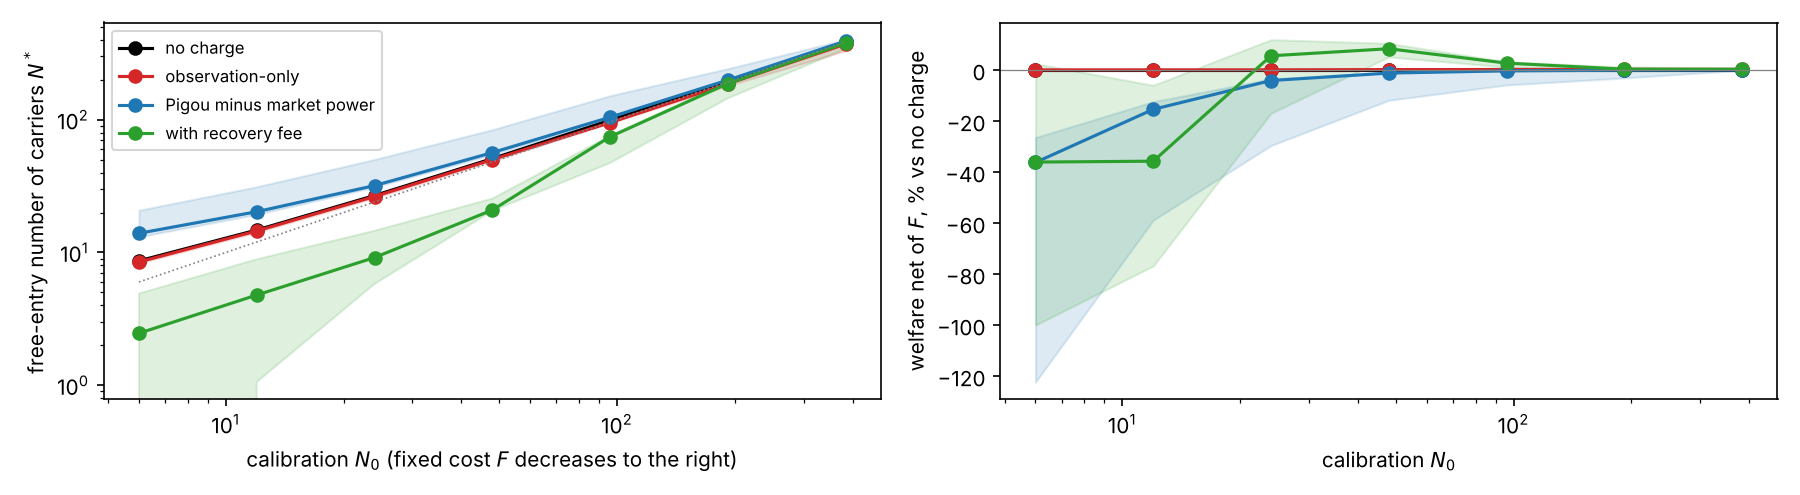
\includegraphics[width=0.88\textwidth]{mfg_entry.png}
\caption{Free entry against the calibration $N_0$ (medians and interquartile ranges; $N_0\in\{6,24,192\}$ over three seeds, the sweep points on seed 0). Left: free-entry number of carriers. Right: welfare net of fixed costs, \% change against no charge.}\label{fig:entry}
\end{figure}

\paragraph{What is not modelled} Fixed costs are not sunk (entry and exit are free, so $N^*$ is a long-run object) and are common within a segment; with heterogeneous fixed costs inframarginal carriers keep rents and the identity of Proposition~\ref{prop:entry}(a) holds only at the margin. The fleet of a segment is fixed; entrants with their own vehicles would add capacity. The count is continuous; the integer constraint \citep{MankiwWhinston1986} moves $N^*$ by less than one carrier per segment.

\subsection{Emissions, noise and through-traffic}\label{sec:extern}
So far the only externality is the delay that delivery vehicles impose on each other while serving a zone; driving between zones is priced only through the tour's own cost. We add emissions, noise and the delay that driving between zones imposes on other traffic as a cost $E_j$ per tour, linear in its vehicle-km:
\[
E_j=\sum_{\text{legs}}\ell_{\rm leg}\big(e_{\rm air}+e_{\rm clim}+e_{\rm noise}\big)+\sum_{\text{legs}}t^0_{\rm leg}\,g(h_{\rm leg})+\sum_{\text{stops}}\ell_{\rm stop}\big(e_{\rm air}+e_{\rm clim}+e_{\rm noise}\big),
\]
with $e_\cdot$ in USD per vehicle-km and welfare $\SW_{\rm ext}=\SW-\sum_i\ip{E_i}{y_i}$. A leg's length $\ell_{\rm leg}$ is the length of the fastest path between the two zone nodes on the major-road graph of the processed city data (the same paths as the travel-time matrix of Section~\ref{sec:data}, reproduced to $10^{-7}$), plus an access drive of 120\,s at each end. The driving between the drops of one stop, $\ell_{\rm stop}=0.7124(A_z\,\mathrm{lot})^{1/2}$, is the Beardwood--Halton--Hammersley length of a tour through $\mathrm{lot}$ points spread over the zone's area $A_z$ \citep{BHH1959}. Through-traffic delay is the marginal external delay of one vehicle under the BPR curve \citep{BPR1964}: a vehicle on a link with free-flow time $t^0$ at congestion level $c$ adds $\beta c\,t^0$ hours of delay to all others, so $g(h)=\mathrm{pce}\,\beta\,\mathrm{cong}(h)\,\mathrm{VOT}$ per free-flow hour of the leg, at the hourly congestion level of Section~\ref{sec:data}. It is charged on inter-zone legs only; delay inside a zone is the $\kappa$ term already in the model. Table~\ref{tab:extparams} lists the values.



\begin{proposition}[Charges for linear tour externalities]\label{prop:extcharge}
Let tour $j$ of carrier $i$ cause the external cost $E_{ij}$, and let $Q'$ be the aggregate of an extended social optimum (maximiser of $\SW_{\rm ext}$).
\begin{enumerate}
\item[(a)] A charge $E_{ij}$ per tour (a distance charge) plus $\kappa\odot Q'$ per delivery makes the mean-field equilibrium an extended optimum; for $N$ identical carriers, a charge $E$ per tour plus $(\kappa-\tfrac mN)\odot Q'$ per delivery makes the Nash equilibrium one.
\item[(b)] If the external cost is additive over deliveries, $E_i=L_i^\top e$ for a common $e\in\R^d$, the per-delivery charge $\kappa\odot Q'+e$ alone does the same in the mean field.
\end{enumerate}
\end{proposition}
\emph{The proof is in Appendix~\ref{app:proofs}.}

Vehicle-km are not proportional to deliveries, so (b) holds only approximately. We compute, in the mean field, the exact rule of (a); the \emph{matched} per-delivery charge that reproduces $Q'$ (damped iteration as in Section~\ref{sec:stake}); and the simple rule $u=\kappa\odot Q'+\bar e$, with $\bar e_k$ the external cost of the tours delivering at $k$ per delivery made there; at finite $N$, the market-power rule with these terms.



\paragraph{Results} Table~\ref{tab:extern} and Figure~\ref{fig:extern}. A delivery drives \ExtVkmDel{} vehicle-km (median; \ExtVkmInShare\,\% of it inside the delivery zones) and causes \ExtPerE{} USD of external cost beyond in-zone delay (city medians \ExtPerEMin--\ExtPerEMax), \ExtShareFee\,\% of the delivery fee (\ExtShareFeeMin--\ExtShareFeeMax\,\%). Through-traffic delay is \ExtShareCong\,\% of it; emissions are \ExtPerAir{} (air) and \ExtPerClim{} (climate) USD per delivery and noise \ExtPerNoise. The external cost is \ExtRatioKQ{} times the in-zone congestion charge $\kappa Q$ (city medians \ExtRatioKQMin--\ExtRatioKQMax). This is the main finding of the extension and a negative one for the model of the earlier sections: the congestion term that the model prices, the delay among delivery vehicles while they serve a zone, is the smaller part of the congestion they cause.

\emph{The charge.} The matched per-delivery charge is \ExtChargeMatch{} USD per delivery against \ExtChargeCong{} for the congestion-only Pigou charge (median ratio \ExtChargeRatio, by city \ExtChargeRatioMin--\ExtChargeRatioMax). At the extended optimum deliveries fall by \ExtDQ\,\% and vehicle-km by \ExtDVkm\,\% (\ExtDVkmPerDel\,\% per delivery: carriers switch to tours with fewer km per drop). \emph{Welfare.} Without a charge the market loses \ExtLossNone\,\% of the optimal welfare of Section~\ref{sec:stake} to the extended optimum (above 20\,\% in New Delhi, Mumbai and London); the congestion-only Pigou charge recovers \ExtGainCongShare\,\% of this gap (at most \ExtGainCongShareMax\,\%), the matched per-delivery charge all but \ExtLossMatch\,\% (at most \ExtLossMatchMax\,\%), and the simple rule $\kappa\odot Q'+\bar e$ all but \ExtLossEbar\,\%: averaging the cost of a tour over its deliveries does not reproduce the optimal aggregate (deliveries \ExtEbarDQ\,\% and vehicle-km \ExtEbarDVkm\,\% against the extended optimum). Zone-hour charges therefore suffice for these externalities if they are set to match the right aggregate; a distance charge adds little. With few carriers market power still dominates: at $N=6$ the losses are \ExtSixNone\,\% (no charge), \ExtSixPmCong\,\% (market-power rule, congestion only), \ExtSixPmMatch\,\% (extended, per delivery) and \ExtSixPmTour\,\% (extended, with distance charge); at $N=1536$ they are \ExtBigNone, \ExtBigPmCong, \ExtBigPmMatch{} and \ExtBigPmTour\,\%.

\emph{Sensitivity.} European values everywhere: \ExtSensEuE{} USD per delivery, no-charge loss \ExtSensEuNone\,\%; Euro~4 air pollution and the EPA carbon value: \ExtSensHiE{} and \ExtSensHiNone\,\%; emissions and noise only: \ExtSensNoCongE{} and \ExtSensNoCongNone\,\%. Emissions and noise alone change the earlier conclusions very little; the through-traffic term carries the result, and its value of time (the driver wage applied to all traffic) is the weakest parameter of Table~\ref{tab:extparams}.

\emph{Exposure.} Assigning each leg's km to the zones its path crosses and each stop's km to its zone, delivery traffic puts \ExpVkmNone{} vehicle-metres per resident and day on the zones it touches (city medians \ExpVkmNoneMin--\ExpVkmNoneMax; \ExpThroughNone\,\% in zones that receive no deliveries), an air-pollution damage of \ExpAirNone{} USD per resident and year (at most \ExpAirMax). This exposure is far less even than the in-zone exposure of Section~\ref{sec:residents}: Gini \ExpGiniNone{} against \ExpBigGiniNone, and a top-to-bottom decile ratio of \ExpDtenNone, consistent with through traffic running on a few corridors. Across served zones it is positively but loosely rank-correlated with the in-zone exposure (Spearman \ExpCorrCong, city medians \ExpCorrCongMin--\ExpCorrCongMax). The extended charge cuts this exposure by \ExpVkmDTour\,\% (congestion-only Pigou: \ExpVkmDCong\,\%) but raises its Gini to \ExpGiniTour{} (higher in \ExpGiniUp{} instances); why the remaining traffic is more concentrated was not tested. Population is the only weight: there are no income or health data, and pollution damage is per vehicle-km, not modelled from concentrations.

\begin{figure}[t]
\centering
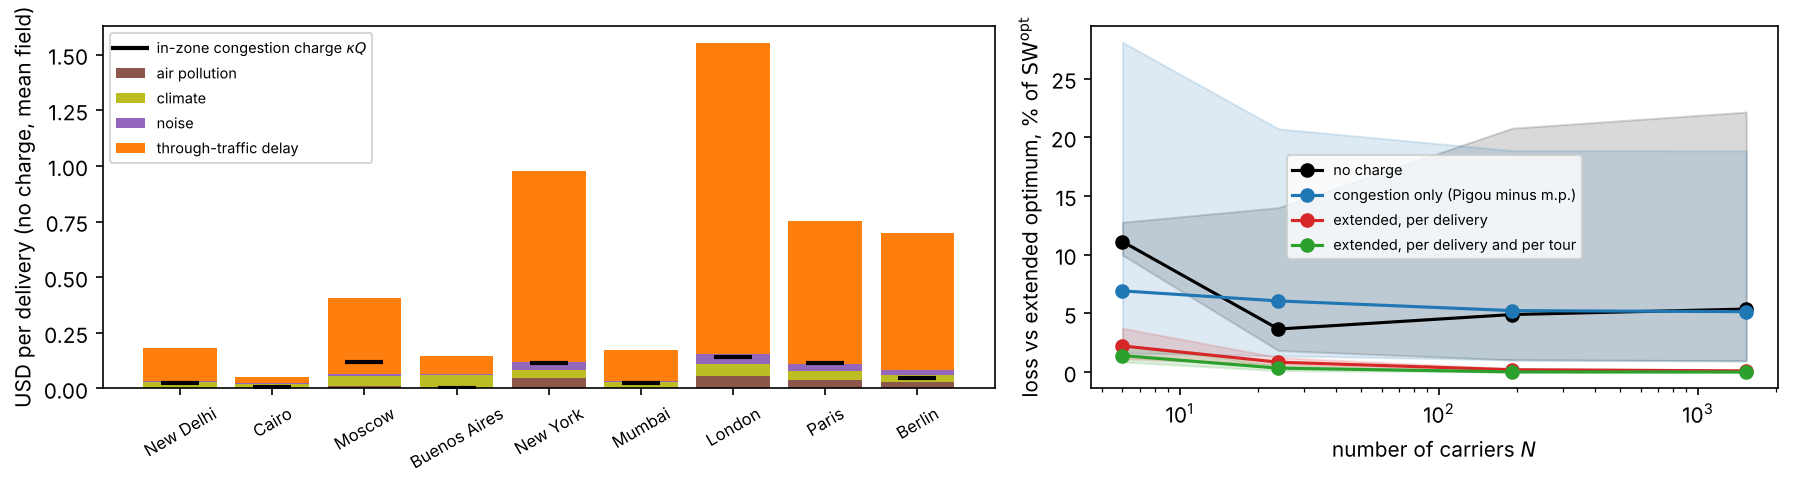
\includegraphics[width=0.88\textwidth]{mfg_extern.png}
\caption{Left: external cost per delivery by component and city (no charge, mean field, median of five seeds), with the in-zone congestion charge $\kappa Q$ (black). Right: welfare below the extended optimum against $N$ (\% of the optimal welfare of Section~\ref{sec:stake}; median and interquartile range over 45 instances).}\label{fig:extern}
\end{figure}


%======================================================================
\section{Discussion}\label{sec:discussion}

\paragraph{What is proved, what is numerically supported, what is open}
Proved, with complete proofs here: Lemmas~\ref{lem:lin}--\ref{lem:rep}, Theorems~\ref{thm:sqrt}, \ref{thm:sep}, \ref{thm:rep}, \ref{thm:toll}, \ref{thm:welfare}, Propositions~\ref{prop:tight}, \ref{prop:common}, \ref{prop:affine}, \ref{prop:arp}, \ref{prop:gamma}, \ref{prop:tod}, \ref{prop:marketpower}, \ref{prop:fee}, \ref{prop:entry}, \ref{prop:extcharge}, \ref{prop:d2} and Corollaries~\ref{cor:poa}, \ref{cor:width}. Theorem~\ref{thm:rep} rests on \citet{Robinson1981}, Proposition~\ref{prop:gamma}(a) and Corollary~\ref{cor:width} on the Omega paper, and Proposition~\ref{prop:arp}(a) restates the Omega contraction theorem. Every bound was also checked by brute force on small random games (Appendix~\ref{app:checks}). Numerically supported only: that the city instances behave like $O(s_N)$ with a constant near one, and that heterogeneous splits do too; that with several carrier types the observation-only charge stays close to the second best under free entry (Proposition~\ref{prop:entry}(d) is for one zone); and all magnitudes of Section~\ref{sec:ext}. Open: an explicit constant for replicas in the polyhedral case, and Conjecture~\ref{conj:d2}.

\paragraph{Who gains and who loses} Section~\ref{sec:stake} splits welfare into carrier profit, consumer surplus, congestion cost and charge revenue. With few carriers the efficient charge is a subsidy that residents (as buyers) and carriers welcome and the council pays for; with many carriers all rules converge to the Pigou charge, which raises a few per cent of welfare and falls on consumers and, in proportion, on carrier profit. The congestion burden for residents is small in the calibration, so the distributional findings are mostly about market power and pass-through. Funding the subsidy from carriers is possible at six carriers only with carrier-specific fees, and once carriers can enter and leave the subsidy buys entrants and the fee drives exits (Section~\ref{sec:ext}).

\paragraph{What the results mean for a city} With many small carriers, a city can set congestion charges from observed zone-hour totals and approach the marginal-cost charge; welfare converges at rate $O(\bar s)$ regardless of how carriers' tours couple zones. With few carriers this rule is harmful, and the market-power correction of the Omega rule is needed. Cautious carriers make an observation-only city over-charge by about their caution margin; the welfare cost is second order. If carriers can enter freely, the market-power subsidy is counterproductive and the plain observation-only charge is the better rule. Most of the external cost of delivery traffic is the delay it causes to other traffic between zones, not the in-zone delay the base model prices; zone-hour charges set to the extended marginal cost and matched to the right aggregate capture nearly all of it.

\paragraph{Limitations} The hourly profile is stylised; real hourly demand and speed data would change the levels in E2--E4 and possibly the economic conclusions, but not the convergence statements. Travel times are deterministic in the experiments (the p-box routing layer of the Omega paper is not re-run on the time-expanded graph, and Proposition~\ref{prop:tod} shows that its corner property can fail with time-dependent charges). In-zone congestion is linear in in-zone hours; driving between zones enters only as a linear external cost on other traffic (Section~\ref{sec:extern}), valued with a proxy value of time, and emissions and noise use unit values per vehicle-km transferred from European estimates. Fixed costs are not sunk and are common within a segment. Tours have at most three stops. The segments are drawn, not observed. The mean-field limit removes market power, which is the economic content of the Omega leader results; for markets with a few large carriers and many small ones, a major-minor model is the right object and is left for later work.

\section{Conclusion}\label{sec:conclusion}
The mean-field limit of competitive urban delivery is reached at rate $O(\bar s)$ when carriers' problems separate across zone-hours, and in the city instances; in the worst case, once tours and fleets couple zones, only the square-root rate holds, and an explicit example attains it. The city's observation-only charge inherits these rates, but its efficiency converges at rate $O(\bar s)$ for every instance. Whether a constant that depends only on the number of zone-hours exists for natural subclasses (unweighted fleet budgets, for example) is the main open question.

\section*{Data and code availability}
Code, instances, result files and the Lean development are in the repository (folder \texttt{mfg}).

\bibliographystyle{elsarticle-harv}
\renewcommand{\bibfont}{\small}\setlength{\bibsep}{1pt plus 0.5pt}
\bibliography{references}

\appendix
\section{Numerical checks of the theory}\label{app:checks}
The script \texttt{mfg/checks/theory\_checks.py} computes, on small random games with linear profits and fleet budgets (and by exhaustive enumeration for pure equilibria of lumpy games), the slack of every inequality of Sections~\ref{sec:model}--\ref{sec:d2}; its output is \texttt{theory\_checks.out}. All slacks were nonnegative (up to the solver accuracy). In particular: the linearisation of Lemma~\ref{lem:pot}(c) reproduces the Nash aggregate to $10^{-7}$; the bound of Theorem~\ref{thm:sqrt}(a) held in 150 games with largest ratio $0.92$; the closed form of Proposition~\ref{prop:tight} matches the solver; Theorem~\ref{thm:sep} held in 200 convexified and 300 lumpy one-zone games (358 pure equilibria), with the constant one attained; Theorem~\ref{thm:sqrt}(b) held on 287 pure equilibria of multi-zone lumpy games.

\section{Machine-checked cores}\label{app:lean}
The Lean~4 file \texttt{mfg/lean/MFG/Core.lean} (Mathlib; no \texttt{sorry}; axioms \texttt{propext}, \texttt{Classical.choice}, \texttt{Quot.sound} only) checks: the symmetric closed form of Theorem~\ref{thm:sep}; the inner-product algebra of Theorem~\ref{thm:sqrt}(a) from the per-carrier optimality inequalities; the revealed-preference and sandwich steps of Theorem~\ref{thm:sep}; the contraction perturbation lemma of Theorem~\ref{thm:toll}; the weighted-norm chain of Proposition~\ref{prop:arp}(a); the algebra of the tightness family (Proposition~\ref{prop:tight}); the welfare inequalities behind Theorem~\ref{thm:welfare}(b) and Proposition~\ref{prop:gamma}(d); the determinant and the weight equivalence of Proposition~\ref{prop:d2}; and the width bound of Corollary~\ref{cor:width}. It does not formalise existence, first-order optimality, Robinson's theorem or the Omega theorems that are used.

\begin{figure}[!ht]
\centering
\begin{minipage}[t]{0.48\textwidth}\centering
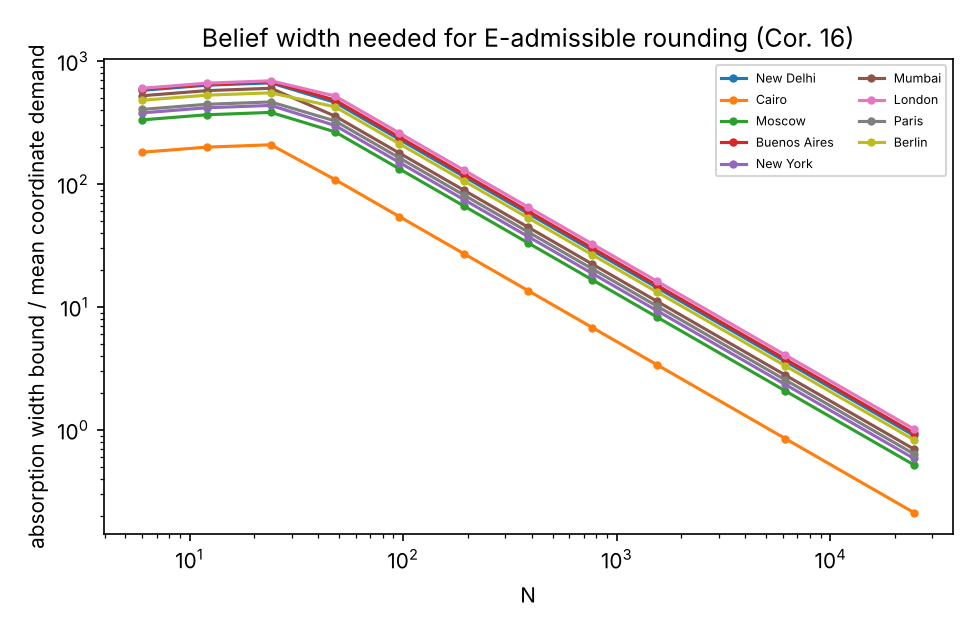
\includegraphics[width=\textwidth]{mfg_width.png}
\caption{Uniform belief width of Corollary~\ref{cor:width} relative to the mean demand of a zone-hour (seed 0).}\label{fig:width}
\end{minipage}\hfill
\begin{minipage}[t]{0.48\textwidth}\centering
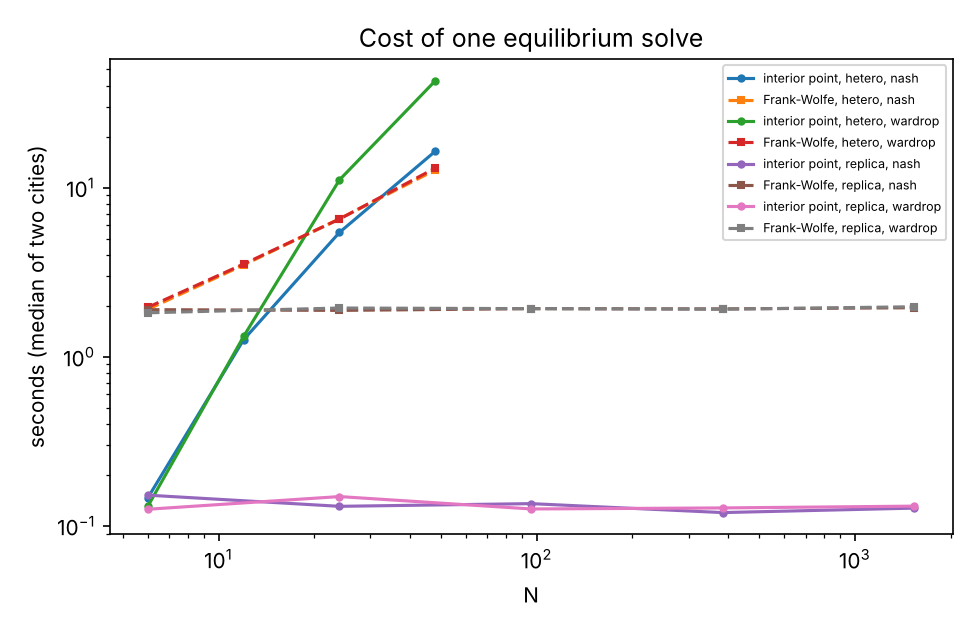
\includegraphics[width=\textwidth]{mfg_cost.png}
\caption{Time of one equilibrium solve (interior point and Frank--Wolfe) for replicas and heterogeneous splits.}\label{fig:cost}
\end{minipage}
\end{figure}

\end{document}
